% mnras_template.tex 
%
% LaTeX template for creating an MNRAS paper
%
% v3.0 released 14 May 2015
% (version numbers match those of mnras.cls)
%
% Copyright (C) Royal Astronomical Society 2015
% Authors:
% Keith T. Smith (Royal Astronomical Society)

% Change log
%
% v3.0 May 2015
%    Renamed to match the new package name
%    Version number matches mnras.cls
%    A few minor tweaks to wording
% v1.0 September 2013
%    Beta testing only - never publicly released
%    First version: a simple (ish) template for creating an MNRAS paper

%%%%%%%%%%%%%%%%%%%%%%%%%%%%%%%%%%%%%%%%%%%%%%%%%%
% Basic setup. Most papers should leave these options alone.
%\documentclass[fleqn,usenatbib]{mnras}
\documentclass[useAMS,usenatbib]{mn2e}

% MNRAS is set in Times font. If you don't have this installed (most LaTeX
% installations will be fine) or prefer the old Computer Modern fonts, comment
% out the following line
%\usepackage{newtxtext,newtxmath}
% Depending on your LaTeX fonts installation, you might get better results with one of these:
%\usepackage{mathptmx}
%\usepackage{txfonts}

% Use vector fonts, so it zooms properly in on-screen viewing software
% Don't change these lines unless you know what you are doing
%\usepackage[T1]{fontenc}

% Allow "Thomas van Noord" and "Simon de Laguarde" and alike to be sorted by "N" and "L" etc. in the bibliography.
% Write the name in the bibliography as "\VAN{Noord}{Van}{van} Noord, Thomas"
%\DeclareRobustCommand{\VAN}[3]{#2}
%\let\VANthebibliography\thebibliography
%\def\thebibliography{\DeclareRobustCommand{\VAN}[3]{##3}\VANthebibliography}


%%%%% AUTHORS - PLACE YOUR OWN PACKAGES HERE %%%%%
%  These Macros are taken from the AAS TeX macro package version 4.0.
%  Include this file in your LaTeX source only if you are not using
%  the AAS TeX macro package and need to resolve the macro definitions
%  in the BibTeX entries returned by the ADS abstract service.
%
%  If you plan not to use this file to resolve the journal macros
%  rather than the whole AAS TeX macro package, you should save the
%  file as ``aas_macros.sty'' and then include it in your paper by
%  using a construct such as:
%\documentstyle[11pt,aas_macros]{article}
%
%  For more information on the AASTeX macro package, please see the URL
%http://www.aas.org/publications/aastex.html
%  For more information about ADS abstract server, please see the URL
%http://adswww.harvard.edu/ads_abstracts.html
%

% Abbreviations for journals.  The object here is to provide authors
% with convenient shorthands for the most ``popular'' (often-cited)
% journals; the author can use these markup tags without being concerned
% about the exact form of the journal abbreviation, or its formatting.
% It is up to the keeper of the macros to make sure the macros expand
% to the proper text.  If macro package writers agree to all use the
% same TeX command name, authors only have to remember one thing, and
% the style file will take care of editorial preferences.  This also
% applies when a single journal decides to revamp its abbreviating
% scheme, as happened with the ApJ (Abt 1991).

\let\jnlstyle=\rm
\def\refjnl#1{{\jnlstyle#1}}

\def\aj{\refjnl{AJ}}                   % Astronomical Journal
\def\araa{\refjnl{ARA\&A}}             % Annual Review of Astron and Astrophys
\def\apj{\refjnl{ApJ}}                 % Astrophysical Journal
\def\apjl{\refjnl{ApJ}}                % Astrophysical Journal, Letters
\def\apjs{\refjnl{ApJS}}               % Astrophysical Journal, Supplement
\def\ao{\refjnl{Appl.~Opt.}}           % Applied Optics
\def\apss{\refjnl{Ap\&SS}}             % Astrophysics and Space Science
\def\aap{\refjnl{A\&A}}                % Astronomy and Astrophysics
\def\aapr{\refjnl{A\&A~Rev.}}          % Astronomy and Astrophysics Reviews
\def\aaps{\refjnl{A\&AS}}              % Astronomy and Astrophysics, Supplement
\def\azh{\refjnl{AZh}}                 % Astronomicheskii Zhurnal
\def\baas{\refjnl{BAAS}}               % Bulletin of the AAS
\def\jrasc{\refjnl{JRASC}}             % Journal of the RAS of Canada
\def\memras{\refjnl{MmRAS}}            % Memoirs of the RAS
\def\mnras{\refjnl{MNRAS}}             % Monthly Notices of the RAS
\def\pra{\refjnl{Phys.~Rev.~A}}        % Physical Review A: General Physics
\def\prb{\refjnl{Phys.~Rev.~B}}        % Physical Review B: Solid State
\def\prc{\refjnl{Phys.~Rev.~C}}        % Physical Review C
\def\prd{\refjnl{Phys.~Rev.~D}}        % Physical Review D
\def\pre{\refjnl{Phys.~Rev.~E}}        % Physical Review E
\def\prl{\refjnl{Phys.~Rev.~Lett.}}    % Physical Review Letters
\def\pasp{\refjnl{PASP}}               % Publications of the ASP
\def\pasj{\refjnl{PASJ}}               % Publications of the ASJ
\def\qjras{\refjnl{QJRAS}}             % Quarterly Journal of the RAS
\def\skytel{\refjnl{S\&T}}             % Sky and Telescope
\def\solphys{\refjnl{Sol.~Phys.}}      % Solar Physics
\def\sovast{\refjnl{Soviet~Ast.}}      % Soviet Astronomy
\def\ssr{\refjnl{Space~Sci.~Rev.}}     % Space Science Reviews
\def\zap{\refjnl{ZAp}}                 % Zeitschrift fuer Astrophysik
\def\nat{\refjnl{Nature}}              % Nature
\def\jcap{\refjnl{JCAP}}          %Journal of Cosmology and Astroparticle Physics
\def\iaucirc{\refjnl{IAU~Circ.}}       % IAU Cirulars
\def\aplett{\refjnl{Astrophys.~Lett.}} % Astrophysics Letters
\def\apspr{\refjnl{Astrophys.~Space~Phys.~Res.}}
                % Astrophysics Space Physics Research
\def\bain{\refjnl{Bull.~Astron.~Inst.~Netherlands}} 
                % Bulletin Astronomical Institute of the Netherlands
\def\fcp{\refjnl{Fund.~Cosmic~Phys.}}  % Fundamental Cosmic Physics
\def\gca{\refjnl{Geochim.~Cosmochim.~Acta}}   % Geochimica Cosmochimica Acta
\def\grl{\refjnl{Geophys.~Res.~Lett.}} % Geophysics Research Letters
\def\jcp{\refjnl{J.~Chem.~Phys.}}      % Journal of Chemical Physics
\def\jgr{\refjnl{J.~Geophys.~Res.}}    % Journal of Geophysics Research
\def\jqsrt{\refjnl{J.~Quant.~Spec.~Radiat.~Transf.}}
                % Journal of Quantitiative Spectroscopy and Radiative Transfer
\def\memsai{\refjnl{Mem.~Soc.~Astron.~Italiana}}
                % Mem. Societa Astronomica Italiana
\def\nphysa{\refjnl{Nucl.~Phys.~A}}   % Nuclear Physics A
\def\physrep{\refjnl{Phys.~Rep.}}   % Physics Reports
\def\physscr{\refjnl{Phys.~Scr}}   % Physica Scripta
\def\planss{\refjnl{Planet.~Space~Sci.}}   % Planetary Space Science
\def\procspie{\refjnl{Proc.~SPIE}}   % Proceedings of the SPIE

\let\astap=\aap
\let\apjlett=\apjl
\let\apjsupp=\apjs
\let\applopt=\ao


% Psfig/TeX 
\def\PsfigVersion{1.9}
% dvips version
%
% All psfig/tex software, documentation, and related files
% in this distribution of psfig/tex are 
% Copyright 1987, 1988, 1991 Trevor J. Darrell
%
% Permission is granted for use and non-profit distribution of psfig/tex 
% providing that this notice is clearly maintained. The right to
% distribute any portion of psfig/tex for profit or as part of any commercial
% product is specifically reserved for the author(s) of that portion.
%
% *** Feel free to make local modifications of psfig as you wish,
% *** but DO NOT post any changed or modified versions of ``psfig''
% *** directly to the net. Send them to me and I'll try to incorporate
% *** them into future versions. If you want to take the psfig code 
% *** and make a new program (subject to the copyright above), distribute it, 
% *** (and maintain it) that's fine, just don't call it psfig.
%
% Bugs and improvements to trevor@media.mit.edu.
%
% Thanks to Greg Hager (GDH) and Ned Batchelder for their contributions
% to the original version of this project.
%
% Modified by J. Daniel Smith on 9 October 1990 to accept the
% %%BoundingBox: comment with or without a space after the colon.  Stole
% file reading code from Tom Rokicki's EPSF.TEX file (see below).
%
% More modifications by J. Daniel Smith on 29 March 1991 to allow the
% the included PostScript figure to be rotated.  The amount of
% rotation is specified by the "angle=" parameter of the \psfig command.
%
% Modified by Robert Russell on June 25, 1991 to allow users to specify
% .ps filenames which don't yet exist, provided they explicitly provide
% boundingbox information via the \psfig command. Note: This will only work
% if the "file=" parameter follows all four "bb???=" parameters in the
% command. This is due to the order in which psfig interprets these params.
%
%  3 Jul 1991	JDS	check if file already read in once
%  4 Sep 1991	JDS	fixed incorrect computation of rotated
%			bounding box
% 25 Sep 1991	GVR	expanded synopsis of \psfig
% 14 Oct 1991	JDS	\fbox code from LaTeX so \psdraft works with TeX
%			changed \typeout to \ps@typeout
% 17 Oct 1991	JDS	added \psscalefirst and \psrotatefirst
%

% From: gvr@cs.brown.edu (George V. Reilly)
%
% \psdraft	draws an outline box, but doesn't include the figure
%		in the DVI file.  Useful for previewing.
%
% \psfull	includes the figure in the DVI file (default).
%
% \psscalefirst width= or height= specifies the size of the figure
% 		before rotation.
% \psrotatefirst (default) width= or height= specifies the size of the
% 		 figure after rotation.  Asymetric figures will
% 		 appear to shrink.
%
% \psfigurepath#1	sets the path to search for the figure
%
% \psfig
% usage: \psfig{file=, figure=, height=, width=,
%			bbllx=, bblly=, bburx=, bbury=,
%			rheight=, rwidth=, clip=, angle=, silent=}
%
%	"file" is the filename.  If no path name is specified and the
%		file is not found in the current directory,
%		it will be looked for in directory \psfigurepath.
%	"figure" is a synonym for "file".
%	By default, the width and height of the figure are taken from
%		the BoundingBox of the figure.
%	If "width" is specified, the figure is scaled so that it has
%		the specified width.  Its height changes proportionately.
%	If "height" is specified, the figure is scaled so that it has
%		the specified height.  Its width changes proportionately.
%	If both "width" and "height" are specified, the figure is scaled
%		anamorphically.
%	"bbllx", "bblly", "bburx", and "bbury" control the PostScript
%		BoundingBox.  If these four values are specified
%               *before* the "file" option, the PSFIG will not try to
%               open the PostScript file.
%	"rheight" and "rwidth" are the reserved height and width
%		of the figure, i.e., how big TeX actually thinks
%		the figure is.  They default to "width" and "height".
%	The "clip" option ensures that no portion of the figure will
%		appear outside its BoundingBox.  "clip=" is a switch and
%		takes no value, but the `=' must be present.
%	The "angle" option specifies the angle of rotation (degrees, ccw).
%	The "silent" option makes \psfig work silently.
%

% check to see if macros already loaded in (maybe some other file says
% "\input psfig") ...
\ifx\undefined\psfig\else\endinput\fi

%
% from a suggestion by eijkhout@csrd.uiuc.edu to allow
% loading as a style file. Changed to avoid problems
% with amstex per suggestion by jbence@math.ucla.edu

\let\LaTeXAtSign=\@
\let\@=\relax
\edef\psfigRestoreAt{\catcode`\@=\number\catcode`@\relax}
%\edef\psfigRestoreAt{\catcode`@=\number\catcode`@\relax}
\catcode`\@=11\relax
\newwrite\@unused
\def\ps@typeout#1{{\let\protect\string\immediate\write\@unused{#1}}}
%\ps@typeout{psfig/tex \PsfigVersion}

%% Here's how you define your figure path.  Should be set up with null
%% default and a user useable definition.

\def\figurepath{./}
\def\psfigurepath#1{\edef\figurepath{#1}}

%
% @psdo control structure -- similar to Latex @for.
% I redefined these with different names so that psfig can
% be used with TeX as well as LaTeX, and so that it will not 
% be vunerable to future changes in LaTeX's internal
% control structure,
%
\def\@nnil{\@nil}
\def\@empty{}
\def\@psdonoop#1\@@#2#3{}
\def\@psdo#1:=#2\do#3{\edef\@psdotmp{#2}\ifx\@psdotmp\@empty \else
    \expandafter\@psdoloop#2,\@nil,\@nil\@@#1{#3}\fi}
\def\@psdoloop#1,#2,#3\@@#4#5{\def#4{#1}\ifx #4\@nnil \else
       #5\def#4{#2}\ifx #4\@nnil \else#5\@ipsdoloop #3\@@#4{#5}\fi\fi}
\def\@ipsdoloop#1,#2\@@#3#4{\def#3{#1}\ifx #3\@nnil 
       \let\@nextwhile=\@psdonoop \else
      #4\relax\let\@nextwhile=\@ipsdoloop\fi\@nextwhile#2\@@#3{#4}}
\def\@tpsdo#1:=#2\do#3{\xdef\@psdotmp{#2}\ifx\@psdotmp\@empty \else
    \@tpsdoloop#2\@nil\@nil\@@#1{#3}\fi}
\def\@tpsdoloop#1#2\@@#3#4{\def#3{#1}\ifx #3\@nnil 
       \let\@nextwhile=\@psdonoop \else
      #4\relax\let\@nextwhile=\@tpsdoloop\fi\@nextwhile#2\@@#3{#4}}
% 
% \fbox is defined in latex.tex; so if \fbox is undefined, assume that
% we are not in LaTeX.
% Perhaps this could be done better???
\ifx\undefined\fbox
% \fbox code from modified slightly from LaTeX
\newdimen\fboxrule
\newdimen\fboxsep
\newdimen\ps@tempdima
\newbox\ps@tempboxa
\fboxsep = 3pt
\fboxrule = .4pt
\long\def\fbox#1{\leavevmode\setbox\ps@tempboxa\hbox{#1}\ps@tempdima\fboxrule
    \advance\ps@tempdima \fboxsep \advance\ps@tempdima \dp\ps@tempboxa
   \hbox{\lower \ps@tempdima\hbox
  {\vbox{\hrule height \fboxrule
          \hbox{\vrule width \fboxrule \hskip\fboxsep
          \vbox{\vskip\fboxsep \box\ps@tempboxa\vskip\fboxsep}\hskip 
                 \fboxsep\vrule width \fboxrule}
                 \hrule height \fboxrule}}}}
\fi
%
%%%%%%%%%%%%%%%%%%%%%%%%%%%%%%%%%%%%%%%%%%%%%%%%%%%%%%%%%%%%%%%%%%%
% file reading stuff from epsf.tex
%   EPSF.TEX macro file:
%   Written by Tomas Rokicki of Radical Eye Software, 29 Mar 1989.
%   Revised by Don Knuth, 3 Jan 1990.
%   Revised by Tomas Rokicki to accept bounding boxes with no
%      space after the colon, 18 Jul 1990.
%   Portions modified/removed for use in PSFIG package by
%      J. Daniel Smith, 9 October 1990.
%
\newread\ps@stream
\newif\ifnot@eof       % continue looking for the bounding box?
\newif\if@noisy        % report what you're making?
\newif\if@atend        % %%BoundingBox: has (at end) specification
\newif\if@psfile       % does this look like a PostScript file?
%
% PostScript files should start with `%!'
%
{\catcode`\%=12\global\gdef\epsf@start{%!}}
\def\epsf@PS{PS}
%
\def\epsf@getbb#1{%
%
%   The first thing we need to do is to open the
%   PostScript file, if possible.
%
\openin\ps@stream=#1
\ifeof\ps@stream\ps@typeout{Error, File #1 not found}\else
%
%   Okay, we got it. Now we'll scan lines until we find one that doesn't
%   start with %. We're looking for the bounding box comment.
%
   {\not@eoftrue \chardef\other=12
    \def\do##1{\catcode`##1=\other}\dospecials \catcode`\ =10
    \loop
       \if@psfile
	  \read\ps@stream to \epsf@fileline
       \else{
	  \obeyspaces
          \read\ps@stream to \epsf@tmp\global\let\epsf@fileline\epsf@tmp}
       \fi
       \ifeof\ps@stream\not@eoffalse\else
%
%   Check the first line for `%!'.  Issue a warning message if its not
%   there, since the file might not be a PostScript file.
%
       \if@psfile\else
       \expandafter\epsf@test\epsf@fileline:. \\%
       \fi
%
%   We check to see if the first character is a % sign;
%   if so, we look further and stop only if the line begins with
%   `%%BoundingBox:' and the `(atend)' specification was not found.
%   That is, the only way to stop is when the end of file is reached,
%   or a `%%BoundingBox: llx lly urx ury' line is found.
%
          \expandafter\epsf@aux\epsf@fileline:. \\%
       \fi
   \ifnot@eof\repeat
   }\closein\ps@stream\fi}%
%
% This tests if the file we are reading looks like a PostScript file.
%
\long\def\epsf@test#1#2#3:#4\\{\def\epsf@testit{#1#2}
			\ifx\epsf@testit\epsf@start\else
\ps@typeout{Warning! File does not start with `\epsf@start'.  It may not be a PostScript file.}
			\fi
			\@psfiletrue} % don't test after 1st line
%
%   We still need to define the tricky \epsf@aux macro. This requires
%   a couple of magic constants for comparison purposes.
%
{\catcode`\%=12\global\let\epsf@percent=%\global\def\epsf@bblit{%BoundingBox}}
%
%
%   So we're ready to check for `%BoundingBox:' and to grab the
%   values if they are found.  We continue searching if `(at end)'
%   was found after the `%BoundingBox:'.
%
\long\def\epsf@aux#1#2:#3\\{\ifx#1\epsf@percent
   \def\epsf@testit{#2}\ifx\epsf@testit\epsf@bblit
	\@atendfalse
        \epsf@atend #3 . \\%
	\if@atend	
	   \if@verbose{
		\ps@typeout{psfig: found `(atend)'; continuing search}
	   }\fi
        \else
        \epsf@grab #3 . . . \\%
        \not@eoffalse
        \global\no@bbfalse
        \fi
   \fi\fi}%
%
%   Here we grab the values and stuff them in the appropriate definitions.
%
\def\epsf@grab #1 #2 #3 #4 #5\\{%
   \global\def\epsf@llx{#1}\ifx\epsf@llx\empty
      \epsf@grab #2 #3 #4 #5 .\\\else
   \global\def\epsf@lly{#2}%
   \global\def\epsf@urx{#3}\global\def\epsf@ury{#4}\fi}%
%
% Determine if the stuff following the %%BoundingBox is `(atend)'
% J. Daniel Smith.  Copied from \epsf@grab above.
%
\def\epsf@atendlit{(atend)} 
\def\epsf@atend #1 #2 #3\\{%
   \def\epsf@tmp{#1}\ifx\epsf@tmp\empty
      \epsf@atend #2 #3 .\\\else
   \ifx\epsf@tmp\epsf@atendlit\@atendtrue\fi\fi}


% End of file reading stuff from epsf.tex
%%%%%%%%%%%%%%%%%%%%%%%%%%%%%%%%%%%%%%%%%%%%%%%%%%%%%%%%%%%%%%%%%%%

%%%%%%%%%%%%%%%%%%%%%%%%%%%%%%%%%%%%%%%%%%%%%%%%%%%%%%%%%%%%%%%%%%%
% trigonometry stuff from "trig.tex"
\chardef\psletter = 11 % won't conflict with \begin{letter} now...
\chardef\other = 12

\newif \ifdebug %%% turn me on to see TeX hard at work ...
\newif\ifc@mpute %%% don't need to compute some values
\c@mputetrue % but assume that we do

\let\then = \relax
\def\r@dian{pt }
\let\r@dians = \r@dian
\let\dimensionless@nit = \r@dian
\let\dimensionless@nits = \dimensionless@nit
\def\internal@nit{sp }
\let\internal@nits = \internal@nit
\newif\ifstillc@nverging
\def \Mess@ge #1{\ifdebug \then \message {#1} \fi}

{ %%% Things that need abnormal catcodes %%%
	\catcode `\@ = \psletter
	\gdef \nodimen {\expandafter \n@dimen \the \dimen}
	\gdef \term #1 #2 #3%
	       {\edef \t@ {\the #1}%%% freeze parameter 1 (count, by value)
		\edef \t@@ {\expandafter \n@dimen \the #2\r@dian}%
				   %%% freeze parameter 2 (dimen, by value)
		\t@rm {\t@} {\t@@} {#3}%
	       }
	\gdef \t@rm #1 #2 #3%
	       {{%
		\count 0 = 0
		\dimen 0 = 1 \dimensionless@nit
		\dimen 2 = #2\relax
		\Mess@ge {Calculating term #1 of \nodimen 2}%
		\loop
		\ifnum	\count 0 < #1
		\then	\advance \count 0 by 1
			\Mess@ge {Iteration \the \count 0 \space}%
			\Multiply \dimen 0 by {\dimen 2}%
			\Mess@ge {After multiplication, term = \nodimen 0}%
			\Divide \dimen 0 by {\count 0}%
			\Mess@ge {After division, term = \nodimen 0}%
		\repeat
		\Mess@ge {Final value for term #1 of 
				\nodimen 2 \space is \nodimen 0}%
		\xdef \Term {#3 = \nodimen 0 \r@dians}%
		\aftergroup \Term
	       }}
	\catcode `\p = \other
	\catcode `\t = \other
	\gdef \n@dimen #1pt{#1} %%% throw away the ``pt''
}

\def \Divide #1by #2{\divide #1 by #2} %%% just a synonym

\def \Multiply #1by #2%%% allows division of a dimen by a dimen
       {{%%% should really freeze parameter 2 (dimen, passed by value)
	\count 0 = #1\relax
	\count 2 = #2\relax
	\count 4 = 65536
	\Mess@ge {Before scaling, count 0 = \the \count 0 \space and
			count 2 = \the \count 2}%
	\ifnum	\count 0 > 32767 %%% do our best to avoid overflow
	\then	\divide \count 0 by 4
		\divide \count 4 by 4
	\else	\ifnum	\count 0 < -32767
		\then	\divide \count 0 by 4
			\divide \count 4 by 4
		\else
		\fi
	\fi
	\ifnum	\count 2 > 32767 %%% while retaining reasonable accuracy
	\then	\divide \count 2 by 4
		\divide \count 4 by 4
	\else	\ifnum	\count 2 < -32767
		\then	\divide \count 2 by 4
			\divide \count 4 by 4
		\else
		\fi
	\fi
	\multiply \count 0 by \count 2
	\divide \count 0 by \count 4
	\xdef \product {#1 = \the \count 0 \internal@nits}%
	\aftergroup \product
       }}

\def\r@duce{\ifdim\dimen0 > 90\r@dian \then   % sin(x+90) = sin(180-x)
		\multiply\dimen0 by -1
		\advance\dimen0 by 180\r@dian
		\r@duce
	    \else \ifdim\dimen0 < -90\r@dian \then  % sin(-x) = sin(360+x)
		\advance\dimen0 by 360\r@dian
		\r@duce
		\fi
	    \fi}

\def\Sine#1%
       {{%
	\dimen 0 = #1 \r@dian
	\r@duce
	\ifdim\dimen0 = -90\r@dian \then
	   \dimen4 = -1\r@dian
	   \c@mputefalse
	\fi
	\ifdim\dimen0 = 90\r@dian \then
	   \dimen4 = 1\r@dian
	   \c@mputefalse
	\fi
	\ifdim\dimen0 = 0\r@dian \then
	   \dimen4 = 0\r@dian
	   \c@mputefalse
	\fi
%
	\ifc@mpute \then
        	% convert degrees to radians
		\divide\dimen0 by 180
		\dimen0=3.141592654\dimen0
%
		\dimen 2 = 3.1415926535897963\r@dian %%% a well-known constant
		\divide\dimen 2 by 2 %%% we only deal with -pi/2 : pi/2
		\Mess@ge {Sin: calculating Sin of \nodimen 0}%
		\count 0 = 1 %%% see power-series expansion for sine
		\dimen 2 = 1 \r@dian %%% ditto
		\dimen 4 = 0 \r@dian %%% ditto
		\loop
			\ifnum	\dimen 2 = 0 %%% then we've done
			\then	\stillc@nvergingfalse 
			\else	\stillc@nvergingtrue
			\fi
			\ifstillc@nverging %%% then calculate next term
			\then	\term {\count 0} {\dimen 0} {\dimen 2}%
				\advance \count 0 by 2
				\count 2 = \count 0
				\divide \count 2 by 2
				\ifodd	\count 2 %%% signs alternate
				\then	\advance \dimen 4 by \dimen 2
				\else	\advance \dimen 4 by -\dimen 2
				\fi
		\repeat
	\fi		
			\xdef \sine {\nodimen 4}%
       }}

% Now the Cosine can be calculated easily by calling \Sine
\def\Cosine#1{\ifx\sine\UnDefined\edef\Savesine{\relax}\else
		             \edef\Savesine{\sine}\fi
	{\dimen0=#1\r@dian\advance\dimen0 by 90\r@dian
	 \Sine{\nodimen 0}
	 \xdef\cosine{\sine}
	 \xdef\sine{\Savesine}}}	      
% end of trig stuff
%%%%%%%%%%%%%%%%%%%%%%%%%%%%%%%%%%%%%%%%%%%%%%%%%%%%%%%%%%%%%%%%%%%%

\def\psdraft{
	\def\@psdraft{0}
	%\ps@typeout{draft level now is \@psdraft \space . }
}
\def\psfull{
	\def\@psdraft{100}
	%\ps@typeout{draft level now is \@psdraft \space . }
}

\psfull

\newif\if@scalefirst
\def\psscalefirst{\@scalefirsttrue}
\def\psrotatefirst{\@scalefirstfalse}
\psrotatefirst

\newif\if@draftbox
\def\psnodraftbox{
	\@draftboxfalse
}
\def\psdraftbox{
	\@draftboxtrue
}
\@draftboxtrue

\newif\if@prologfile
\newif\if@postlogfile
\def\pssilent{
	\@noisyfalse
}
\def\psnoisy{
	\@noisytrue
}
\psnoisy
%%% These are for the option list.
%%% A specification of the form a = b maps to calling \@p@@sa{b}
\newif\if@bbllx
\newif\if@bblly
\newif\if@bburx
\newif\if@bbury
\newif\if@height
\newif\if@width
\newif\if@rheight
\newif\if@rwidth
\newif\if@angle
\newif\if@clip
\newif\if@verbose
\def\@p@@sclip#1{\@cliptrue}


\newif\if@decmpr

%%% GDH 7/26/87 -- changed so that it first looks in the local directory,
%%% then in a specified global directory for the ps file.
%%% RPR 6/25/91 -- changed so that it defaults to user-supplied name if
%%% boundingbox info is specified, assuming graphic will be created by
%%% print time.
%%% TJD 10/19/91 -- added bbfile vs. file distinction, and @decmpr flag

\def\@p@@sfigure#1{\def\@p@sfile{null}\def\@p@sbbfile{null}
	        \openin1=#1.bb
		\ifeof1\closein1
	        	\openin1=\figurepath#1.bb
			\ifeof1\closein1
			        \openin1=#1
				\ifeof1\closein1%
				       \openin1=\figurepath#1
					\ifeof1
					   \ps@typeout{Error, File #1 not found}
						\if@bbllx\if@bblly
				   		\if@bburx\if@bbury
			      				\def\@p@sfile{#1}%
			      				\def\@p@sbbfile{#1}%
							\@decmprfalse
				  	   	\fi\fi\fi\fi
					\else\closein1
				    		\def\@p@sfile{\figurepath#1}%
				    		\def\@p@sbbfile{\figurepath#1}%
						\@decmprfalse
	                       		\fi%
			 	\else\closein1%
					\def\@p@sfile{#1}
					\def\@p@sbbfile{#1}
					\@decmprfalse
			 	\fi
			\else
				\def\@p@sfile{\figurepath#1}
				\def\@p@sbbfile{\figurepath#1.bb}
				\@decmprtrue
			\fi
		\else
			\def\@p@sfile{#1}
			\def\@p@sbbfile{#1.bb}
			\@decmprtrue
		\fi}

\def\@p@@sfile#1{\@p@@sfigure{#1}}

\def\@p@@sbbllx#1{
		%\ps@typeout{bbllx is #1}
		\@bbllxtrue
		\dimen100=#1
		\edef\@p@sbbllx{\number\dimen100}
}
\def\@p@@sbblly#1{
		%\ps@typeout{bblly is #1}
		\@bbllytrue
		\dimen100=#1
		\edef\@p@sbblly{\number\dimen100}
}
\def\@p@@sbburx#1{
		%\ps@typeout{bburx is #1}
		\@bburxtrue
		\dimen100=#1
		\edef\@p@sbburx{\number\dimen100}
}
\def\@p@@sbbury#1{
		%\ps@typeout{bbury is #1}
		\@bburytrue
		\dimen100=#1
		\edef\@p@sbbury{\number\dimen100}
}
\def\@p@@sheight#1{
		\@heighttrue
		\dimen100=#1
   		\edef\@p@sheight{\number\dimen100}
		%\ps@typeout{Height is \@p@sheight}
}
\def\@p@@swidth#1{
		%\ps@typeout{Width is #1}
		\@widthtrue
		\dimen100=#1
		\edef\@p@swidth{\number\dimen100}
}
\def\@p@@srheight#1{
		%\ps@typeout{Reserved height is #1}
		\@rheighttrue
		\dimen100=#1
		\edef\@p@srheight{\number\dimen100}
}
\def\@p@@srwidth#1{
		%\ps@typeout{Reserved width is #1}
		\@rwidthtrue
		\dimen100=#1
		\edef\@p@srwidth{\number\dimen100}
}
\def\@p@@sangle#1{
		%\ps@typeout{Rotation is #1}
		\@angletrue
%		\dimen100=#1
		\edef\@p@sangle{#1} %\number\dimen100}
}
\def\@p@@ssilent#1{ 
		\@verbosefalse
}
\def\@p@@sprolog#1{\@prologfiletrue\def\@prologfileval{#1}}
\def\@p@@spostlog#1{\@postlogfiletrue\def\@postlogfileval{#1}}
\def\@cs@name#1{\csname #1\endcsname}
\def\@setparms#1=#2,{\@cs@name{@p@@s#1}{#2}}
%
% initialize the defaults (size the size of the figure)
%
\def\ps@init@parms{
		\@bbllxfalse \@bbllyfalse
		\@bburxfalse \@bburyfalse
		\@heightfalse \@widthfalse
		\@rheightfalse \@rwidthfalse
		\def\@p@sbbllx{}\def\@p@sbblly{}
		\def\@p@sbburx{}\def\@p@sbbury{}
		\def\@p@sheight{}\def\@p@swidth{}
		\def\@p@srheight{}\def\@p@srwidth{}
		\def\@p@sangle{0}
		\def\@p@sfile{} \def\@p@sbbfile{}
		\def\@p@scost{10}
		\def\@sc{}
		\@prologfilefalse
		\@postlogfilefalse
		\@clipfalse
		\if@noisy
			\@verbosetrue
		\else
			\@verbosefalse
		\fi
}
%
% Go through the options setting things up.
%
\def\parse@ps@parms#1{
	 	\@psdo\@psfiga:=#1\do
		   {\expandafter\@setparms\@psfiga,}}
%
% Compute bb height and width
%
\newif\ifno@bb
\def\bb@missing{
	\if@verbose{
		\ps@typeout{psfig: searching \@p@sbbfile \space  for bounding box}
	}\fi
	\no@bbtrue
	\epsf@getbb{\@p@sbbfile}
        \ifno@bb \else \bb@cull\epsf@llx\epsf@lly\epsf@urx\epsf@ury\fi
}	
\def\bb@cull#1#2#3#4{
	\dimen100=#1 bp\edef\@p@sbbllx{\number\dimen100}
	\dimen100=#2 bp\edef\@p@sbblly{\number\dimen100}
	\dimen100=#3 bp\edef\@p@sbburx{\number\dimen100}
	\dimen100=#4 bp\edef\@p@sbbury{\number\dimen100}
	\no@bbfalse
}
% rotate point (#1,#2) about (0,0).
% The sine and cosine of the angle are already stored in \sine and
% \cosine.  The result is placed in (\p@intvaluex, \p@intvaluey).
\newdimen\p@intvaluex
\newdimen\p@intvaluey
\def\rotate@#1#2{{\dimen0=#1 sp\dimen1=#2 sp
%            	calculate x' = x \cos\theta - y \sin\theta
		  \global\p@intvaluex=\cosine\dimen0
		  \dimen3=\sine\dimen1
		  \global\advance\p@intvaluex by -\dimen3
% 		calculate y' = x \sin\theta + y \cos\theta
		  \global\p@intvaluey=\sine\dimen0
		  \dimen3=\cosine\dimen1
		  \global\advance\p@intvaluey by \dimen3
		  }}
\def\compute@bb{
		\no@bbfalse
		\if@bbllx \else \no@bbtrue \fi
		\if@bblly \else \no@bbtrue \fi
		\if@bburx \else \no@bbtrue \fi
		\if@bbury \else \no@bbtrue \fi
		\ifno@bb \bb@missing \fi
		\ifno@bb \ps@typeout{FATAL ERROR: no bb supplied or found}
			\no-bb-error
		\fi
		%
%\ps@typeout{BB: \@p@sbbllx, \@p@sbblly, \@p@sbburx, \@p@sbbury} 
%
% store height/width of original (unrotated) bounding box
		\count203=\@p@sbburx
		\count204=\@p@sbbury
		\advance\count203 by -\@p@sbbllx
		\advance\count204 by -\@p@sbblly
		\edef\ps@bbw{\number\count203}
		\edef\ps@bbh{\number\count204}
		%\ps@typeout{ psbbh = \ps@bbh, psbbw = \ps@bbw }
		\if@angle 
			\Sine{\@p@sangle}\Cosine{\@p@sangle}
	        	{\dimen100=\maxdimen\xdef\r@p@sbbllx{\number\dimen100}
					    \xdef\r@p@sbblly{\number\dimen100}
			                    \xdef\r@p@sbburx{-\number\dimen100}
					    \xdef\r@p@sbbury{-\number\dimen100}}
%
% Need to rotate all four points and take the X-Y extremes of the new
% points as the new bounding box.
                        \def\minmaxtest{
			   \ifnum\number\p@intvaluex<\r@p@sbbllx
			      \xdef\r@p@sbbllx{\number\p@intvaluex}\fi
			   \ifnum\number\p@intvaluex>\r@p@sbburx
			      \xdef\r@p@sbburx{\number\p@intvaluex}\fi
			   \ifnum\number\p@intvaluey<\r@p@sbblly
			      \xdef\r@p@sbblly{\number\p@intvaluey}\fi
			   \ifnum\number\p@intvaluey>\r@p@sbbury
			      \xdef\r@p@sbbury{\number\p@intvaluey}\fi
			   }
%			lower left
			\rotate@{\@p@sbbllx}{\@p@sbblly}
			\minmaxtest
%			upper left
			\rotate@{\@p@sbbllx}{\@p@sbbury}
			\minmaxtest
%			lower right
			\rotate@{\@p@sbburx}{\@p@sbblly}
			\minmaxtest
%			upper right
			\rotate@{\@p@sbburx}{\@p@sbbury}
			\minmaxtest
			\edef\@p@sbbllx{\r@p@sbbllx}\edef\@p@sbblly{\r@p@sbblly}
			\edef\@p@sbburx{\r@p@sbburx}\edef\@p@sbbury{\r@p@sbbury}
%\ps@typeout{rotated BB: \r@p@sbbllx, \r@p@sbblly, \r@p@sbburx, \r@p@sbbury}
		\fi
		\count203=\@p@sbburx
		\count204=\@p@sbbury
		\advance\count203 by -\@p@sbbllx
		\advance\count204 by -\@p@sbblly
		\edef\@bbw{\number\count203}
		\edef\@bbh{\number\count204}
		%\ps@typeout{ bbh = \@bbh, bbw = \@bbw }
}
%
% \in@hundreds performs #1 * (#2 / #3) correct to the hundreds,
%	then leaves the result in @result
%
\def\in@hundreds#1#2#3{\count240=#2 \count241=#3
		     \count100=\count240	% 100 is first digit #2/#3
		     \divide\count100 by \count241
		     \count101=\count100
		     \multiply\count101 by \count241
		     \advance\count240 by -\count101
		     \multiply\count240 by 10
		     \count101=\count240	%101 is second digit of #2/#3
		     \divide\count101 by \count241
		     \count102=\count101
		     \multiply\count102 by \count241
		     \advance\count240 by -\count102
		     \multiply\count240 by 10
		     \count102=\count240	% 102 is the third digit
		     \divide\count102 by \count241
		     \count200=#1\count205=0
		     \count201=\count200
			\multiply\count201 by \count100
		 	\advance\count205 by \count201
		     \count201=\count200
			\divide\count201 by 10
			\multiply\count201 by \count101
			\advance\count205 by \count201
			%
		     \count201=\count200
			\divide\count201 by 100
			\multiply\count201 by \count102
			\advance\count205 by \count201
			%
		     \edef\@result{\number\count205}
}
\def\compute@wfromh{
		% computing : width = height * (bbw / bbh)
		\in@hundreds{\@p@sheight}{\@bbw}{\@bbh}
		%\ps@typeout{ \@p@sheight * \@bbw / \@bbh, = \@result }
		\edef\@p@swidth{\@result}
		%\ps@typeout{w from h: width is \@p@swidth}
}
\def\compute@hfromw{
		% computing : height = width * (bbh / bbw)
	        \in@hundreds{\@p@swidth}{\@bbh}{\@bbw}
		%\ps@typeout{ \@p@swidth * \@bbh / \@bbw = \@result }
		\edef\@p@sheight{\@result}
		%\ps@typeout{h from w : height is \@p@sheight}
}
\def\compute@handw{
		\if@height 
			\if@width
			\else
				\compute@wfromh
			\fi
		\else 
			\if@width
				\compute@hfromw
			\else
				\edef\@p@sheight{\@bbh}
				\edef\@p@swidth{\@bbw}
			\fi
		\fi
}
\def\compute@resv{
		\if@rheight \else \edef\@p@srheight{\@p@sheight} \fi
		\if@rwidth \else \edef\@p@srwidth{\@p@swidth} \fi
		%\ps@typeout{rheight = \@p@srheight, rwidth = \@p@srwidth}
}
%		
% Compute any missing values
\def\compute@sizes{
	\compute@bb
	\if@scalefirst\if@angle
% at this point the bounding box has been adjsuted correctly for
% rotation.  PSFIG does all of its scaling using \@bbh and \@bbw.  If
% a width= or height= was specified along with \psscalefirst, then the
% width=/height= value needs to be adjusted to match the new (rotated)
% bounding box size (specifed in \@bbw and \@bbh).
%    \ps@bbw       width=
%    -------  =  ---------- 
%    \@bbw       new width=
% so `new width=' = (width= * \@bbw) / \ps@bbw; where \ps@bbw is the
% width of the original (unrotated) bounding box.
	\if@width
	   \in@hundreds{\@p@swidth}{\@bbw}{\ps@bbw}
	   \edef\@p@swidth{\@result}
	\fi
	\if@height
	   \in@hundreds{\@p@sheight}{\@bbh}{\ps@bbh}
	   \edef\@p@sheight{\@result}
	\fi
	\fi\fi
	\compute@handw
	\compute@resv}

%
% \psfig
% usage : \psfig{file=, height=, width=, bbllx=, bblly=, bburx=, bbury=,
%			rheight=, rwidth=, clip=}
%
% "clip=" is a switch and takes no value, but the `=' must be present.
\def\psfig#1{\vbox {
	% do a zero width hard space so that a single
	% \psfig in a centering enviornment will behave nicely
	%{\setbox0=\hbox{\ }\ \hskip-\wd0}
	%
	\ps@init@parms
	\parse@ps@parms{#1}
	\compute@sizes
	%
	\ifnum\@p@scost<\@psdraft{
		%
		\special{ps::[begin] 	\@p@swidth \space \@p@sheight \space
				\@p@sbbllx \space \@p@sbblly \space
				\@p@sbburx \space \@p@sbbury \space
				startTexFig \space }
		\if@angle
			\special {ps:: \@p@sangle \space rotate \space} 
		\fi
		\if@clip{
			\if@verbose{
				\ps@typeout{(clip)}
			}\fi
			\special{ps:: doclip \space }
		}\fi
		\if@prologfile
		    \special{ps: plotfile \@prologfileval \space } \fi
		\if@decmpr{
			\if@verbose{
				\ps@typeout{psfig: including \@p@sfile.Z \space }
			}\fi
			\special{ps: plotfile "`zcat \@p@sfile.Z" \space }
		}\else{
			\if@verbose{
				\ps@typeout{psfig: including \@p@sfile \space }
			}\fi
			\special{ps: plotfile \@p@sfile \space }
		}\fi
		\if@postlogfile
		    \special{ps: plotfile \@postlogfileval \space } \fi
		\special{ps::[end] endTexFig \space }
		% Create the vbox to reserve the space for the figure.
		\vbox to \@p@srheight sp{
		% 1/92 TJD Changed from "true sp" to "sp" for magnification.
			\hbox to \@p@srwidth sp{
				\hss
			}
		\vss
		}
	}\else{
		% draft figure, just reserve the space and print the
		% path name.
		\if@draftbox{		
			% Verbose draft: print file name in box
			\hbox{\frame{\vbox to \@p@srheight sp{
			\vss
			\hbox to \@p@srwidth sp{ \hss \@p@sfile \hss }
			\vss
			}}}
		}\else{
			% Non-verbose draft
			\vbox to \@p@srheight sp{
			\vss
			\hbox to \@p@srwidth sp{\hss}
			\vss
			}
		}\fi	



	}\fi
}}
\psfigRestoreAt
\let\@=\LaTeXAtSign





\usepackage{graphicx}
\usepackage{epsfig}
\usepackage{amssymb}
\usepackage{amsmath}
\usepackage{amsfonts}
\usepackage{txfonts}
\usepackage{multirow}
\usepackage{afterpage}
\usepackage{xcolor}
\usepackage{orcidlink}
\usepackage{xspace}
%\usepackage[draft]{hyperref}
%\usepackage{ulem} % allows for strikethrough with \sout{}


%\usepackage[paperheight=10in,paperwidth=8.5in]{geometry}

\setlength{\topmargin}{-0.8in}
\paperheight 11in
\paperwidth 8.5in
%\setlength{\textheight}{9.8in}
%\setlength{\textwidth}{7.3in}
\setlength{\textheight}{9.5in}
\setlength{\textwidth}{7.1in}

\definecolor{mypink1}{rgb}{0.858, 0.188, 0.478}
\definecolor{mygreen1}{rgb}{0.258, 0.788, 0.878}
\definecolor{myorange1}{rgb}{0.5, 0.2, 0.2}
\newcommand{\NM}[1]{\textcolor[RGB]{0,150,0}{#1}}
\newcommand{\RR}[1]{\textcolor{blue}{#1}}
\newcommand{\JHD}[1]{\textcolor{mypink1}{#1}}
\newcommand{\niko}[1]{\textcolor{orange}{niko: #1}}
\newcommand{\snr}{$\mathcal{S}/\mathcal{N}$ }
\newcommand{\mycomment}[1]{}
\newcommand{\dNLA}{extended\text{-NLA}\xspace}
\newcommand{\dTT}{extended\text{-TT}\xspace}
\newcommand{\gtwopcf}{$\gamma$\text{-2PCF}\xspace}
\newcommand{\eg}{\textit{e.g.}\xspace}
\newcommand{\ie}{\textit{i.e.}\xspace}
\newcommand{\lcdm}{$\Lambda$CDM\xspace}




%%%%%%%%%%%%%%%%%%%%%%%%%%%%%%%%%%%%%%%%%%%%%%%%%%

%%%%% AUTHORS - PLACE YOUR OWN COMMANDS HERE %%%%%

% Please keep new commands to a minimum, and use \newcommand not \def to avoid
% overwriting existing commands. Example:
%\newcommand{\pcm}{\,cm$^{-2}$}	% per cm-squared

%%%%%%%%%%%%%%%%%%%%%%%%%%%%%%%%%%%%%%%%%%%%%%%%%%

%%%%%%%%%%%%%%%%%%% TITLE PAGE %%%%%%%%%%%%%%%%%%%

% Title of the paper, and the short title which is used in the headers.
% Keep the title short and informative.
\title[Lensing beyond 2pt: accounting for IA]{Intrinsic alignments from projected tidal fields: non-linear  impact on cosmic shear probes}

% The list of authors, and the short list which is used in the headers.
% If you need two or more lines of authors, add an extra line using \newauthor
\author[J. Harnois-D\'{e}raps et al.]{Joachim Harnois-D\'{e}raps$^{1}$
\orcidlink{0000-0002-4864-1240}
\thanks{E-mail: joachim.harnois-deraps@ncl.ac.uk},
Nikolina \v{S}ar\v{c}evi\'c,$^{1}$
\orcidlink{0000-0001-7301-6415},
and others
\newauthor
and the LSST Dark Energy Science Collaboration
\\
% List of institutions
$^{1}$School of Mathematics, Statistics and Physics, Newcastle University, Herschel Building, NE1 7RU, Newcastle-upon-Tyne, UK\\
}

% These dates will be filled out by the publisher
\date{Accepted XXX. Received YYY; in original form ZZZ}

% Enter the current year, for the copyright statements etc.
\pubyear{2024}

% Don't change these lines
\begin{document}
\label{firstpage}
\pagerange{\pageref{firstpage}--21}
%\pagerange{\pageref{firstpage}--\pageref{lastpage}}
\maketitle

% Abstract of the paper

\begin{abstract}
We present the results of our work on intrinsic alignments from tidal fields and the nonlinear impact on cosmic shear probes.
...
\end{abstract}

% Select between one and six entries from the list of approved keywords.
% Don't make up new ones.
\begin{keywords}
Gravitational lensing: weak -- Methods: numerical -- Cosmology: dark matter, dark energy \& large-scale structure of Universe 
\end{keywords}

%%%%%%%%%%%%%%%%%%%%%%%%%%%%%%%%%%%%%%%%%%%%%%%%%%

%%%%%%%%%%%%%%%%% BODY OF PAPER %%%%%%%%%%%%%%%%%%

%----------
\section{Introduction}
\label{sec:intro}
%----------

Recent cosmic shear measurements from the Kilo Degree Survey\footnote{KiDS:kids.strw.leidenuniv.nl}, the Dark Energy Survey\footnote{DES:www.darkenergysurvey.org}, and the Hyper Suprime Camera Survey\footnote{HSC:www.naoj.org/Projects/HSC} have established weak gravitational lensing as a competitive probe of cosmology \citep[see. \eg][]{KiDS1000_Asgari, KiDS1000_vdB, KiDS1000_Li, DESY3_Secco, DESY3_Amon, HSCY3_Cl, HSCY3_2pcf}, achieving  percent-level measurements of the structure growth parameter $S_8\equiv\sigma_8\sqrt{\Omega_{\rm m}/0.3}$.
The parameters $\Omega_{\rm m}$ and $\sigma_8$, which respectively describe the abundance and the amplitude of the fluctuations in the matter density fluctuations on scales of $8h^{-1}$ Mpc, are highly degenerate in the lensing signal, and additional data (\eg galaxy clustering data) are required to measure the two individually from photometric galaxy surveys \citep{KiDS1000_Heymans, DESY3_3x2, HSCY3_3x2}.
Despite these successful achievements, the current precision of cosmic shear cosmology is mainly limited by the large uncertainty in the intrinsic alignment (IA) of galaxies, a secondary signal that tends to cancel some of the shape correlations produced by lensing \citep[see. \eg][for reviews on IA]{Troxel_IA_review_2015, Kirk_IA_review_2015, Joachimi_IA_review_2015, Kiessling_IA_review_2015,Lamman_IA_guide}. 
If unaccounted for, the IA can bias by 4-5$\sigma$ the inferred cosmological parameters \citep{Kirk2012, Krause2016}.
Additionally, using an inaccurate IA model can substantially impair the inference process, as demonstrated by \citet{DESY3_Secco} in their study on DES-Y3 analysis and by \citet{Paopiamsap2024} in the context of an LSST-like cosmic shear analysis.
%Furthermore, an incorrect IA model can also cause significant damage to the inference, as shown in \citet{DESY3_Secco} in the context of DES-Y3 analysis, or in \citep{Paopiamsap2024} in the context of an LSST-like cosmic shear analysis. 

Different physical models have been developed to describe the origin and impact of the IA, including the linear non-linear alignment model \citep[NLA hereafter, ][]{NLA}, the density-weighted NLA (aka $\delta$-NLA or extended-NLA), and the tidal torque model \citep[][TT hereafter]{TATT}, which respectively assume a linear and quadratic coupling between galaxy ellipticities and the local tidal field. 
Alternatively, the halo model can also describe the IA signal as a function of halo properties such as their mass, concentration, and shapes \citep{Fortuna2020}.
A number of observations have sought to place constraints on the parameters from these models \citep[\eg][]{BlueIA, Singh_IA_LOWZ, DESY1_IA_Samuroff, Johnston_IA} {(\it any more recent?)}.
These observations seem to converge towards a strong colour-dependence: red bright galaxies (often elliptical) are generally strongly aligned, with hints of a radial dependence, while blue galaxies (typically spiral) are consistent with the no-alignment scenario.
%A number of observations have sought to place constraints on the parameters from these models \citep[\eg][]{Singh, Sammuroff, Sammuroff, Christos, Fortuna, Johnston}, which seem to converge towards a strong colour-dependence (red bright galaxies are generally strongly aligned, with hints of a radial dependence), while blue galaxies are consistent with the no-alignment scenario.
The selection effects play a crucial role, making it difficult to generalise these measurements to a different galaxy sample, therefore leaving behind a large uncertainty on the IA parameters.


While most theoretical methods have been developed to provide prescriptions for modelling IA in two-point statistics, some have been applied to infuse galaxy alignments directly into cosmological simulations, as in \citet{Fluri2019, Tidalator2D, MICE_IA, Lanzieri2023, vanAlfen2023}. 
Access to such IA-infused numerical simulations is crucial for several applications, including 
validating theoretical models deep in the non-linear regime or utilising non-linear galaxy bias model \citep{IA_gal_bias}, 
 predicting the impact of IA on non-Gaussian lensing probes ({\it i.e.} beyond-2pt statistics), for which no models exist \citep{Zuercher2020a, Tidalator2D},
testing IA mitigation techniques such as self-calibration \citep[][Bera et al in prep.]{SelfCalibrationYao1, SelfCalibrationYao2, SelCalibrationPedersen} or exploring the connection between large dark matter haloes and IA \citep{vanAlfen2023}.
{\JHD{ (Any other important references?)}} These are all important if we are to correctly interpret the cosmological data from photometric redshift surveys. 

This paper addresses several of the above-mentioned applications, as we present a novel  pipeline with which we infuse the NLAl, the \dNLA, and the TT model on the same underlying large lensing simulation. 
In addition, we introduce the \dTT model (which takes into account the fact that galaxies trace dark matter even in the TT model), then proceed to couple the cosmic tidal fields with galaxies taken from halo occupation distributions (HOD), thereby probing the impact of realistic non-linear galaxy bias on the IA signal. These new models are both physically motivated and challenging to describe theoretically as they require perturbation expansions beyond the second order.  Existing  beyond-2pt analyses of weak lensing data only model the NLA model \citep{DESY3_Zuercher, HD21}, which is bound to be insufficient with the precision increase provided with the new generation of cosmic shear surveys such as those from the Vera Rubin Observatory \citep{LSST-Design} or {\it Euclid} \citep{RedBook}. 

After reviewing the theory and measurement of cosmic shear data in Sec. \ref{sec:theory}, we describe our IA models in Sec. \ref{sec:IA_th}.  
Their full numerical implementation is described in Sec. \ref{sec:sims} and validated against theoretical predictions at the level of  two-point shear correlation functions in Sec. \ref{sec:validation}.
Since our infusion method acts on shear galaxy catalogues and on convergence maps, we are in an ideal position to quantify the impact of multiple IA models on different non-Gaussian statistics, which we report in Sec. \ref{sec:HOWLS}, before concluding in Sec. \ref{sec:conclusion}.  
\section{Cosmic shear statistics}
\label{sec:theory}

Cosmic shear data can be analysed using various summary statistics, each with its own advantages and disadvantages.
%Cosmic shear data can be analysed by a number of summary statistics, which all have their pros and cons.
We start with shear two-point functions, then present other complementary cosmic shear statistics in the second part of this section.

%-------------------------
\subsection{$\gamma$-2PCF}
\label{subsec:wl-th}

\begin{figure}
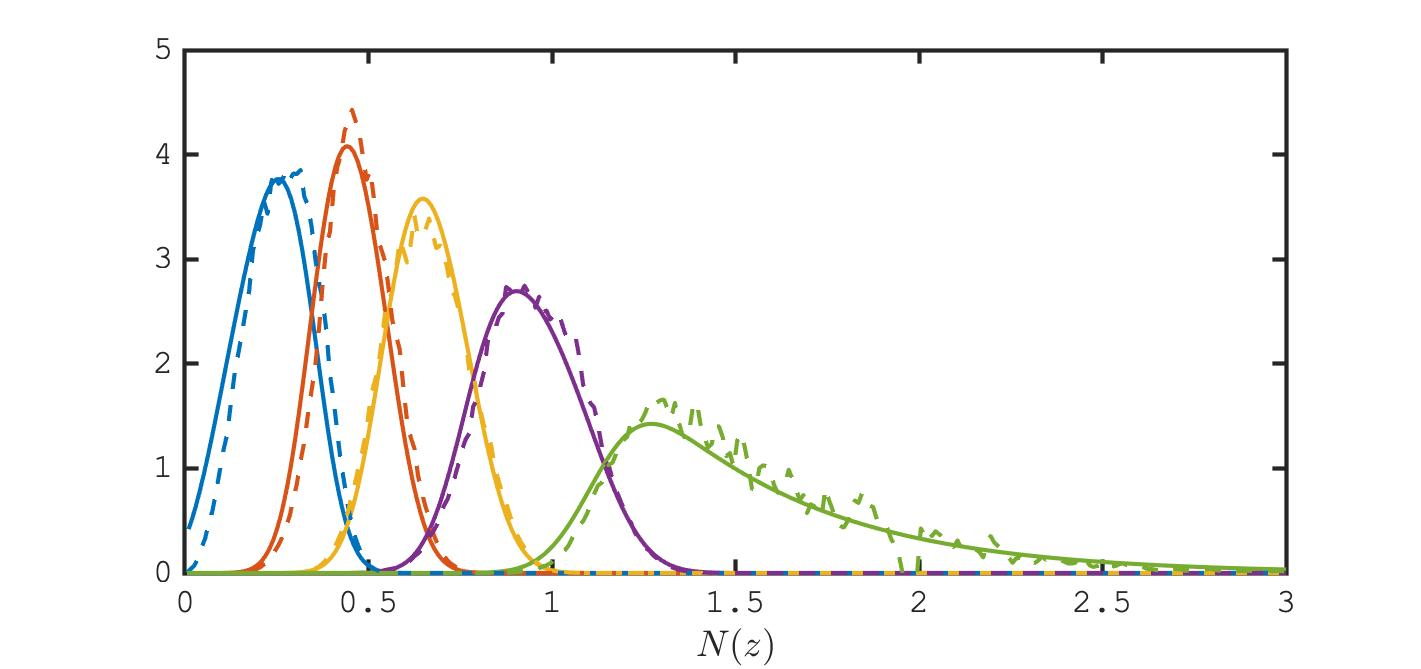
\includegraphics[width=\columnwidth]{graphs/Nz}
\caption{Tomographic redshift distributions in our simulations, either taken from the Year-1 specifications for LSST (solid) or from a matched selection applied to an HOD galaxy catalogue (dashed, see Sec. \ref{subsec:HOD}).}
\label{fig:Nz}
\end{figure}

Shear two-point correlation functions (\gtwopcf hereafter) can be predicted with percent-level precision and are therefore an ideal quantity to validate weak lensing simulations.
In the Limber approximation\footnote{See \citet{Kilbinger17} for a comparison between the Limber approximation and the exact calculations.}, the tomographic lensing power spectrum $C^{ij}_{\ell}$, obtained for combinations of redshift bins $i$ and $j$, is calculated from an integral over the three-dimensional matter power spectrum $P_{\delta}(k, z)$ as:
  \begin{eqnarray}
C_{\ell}^{ij} = \int_0^{\chi_{\rm H}}  \frac{q^i(\chi) \,q^j(\chi)}{\chi^2} \, P_{\delta}\, \bigg(\frac{\ell+1/2}{\chi},z(\chi)\bigg) \ {\rm d}\chi,
\label{eq:C_ell}
\end{eqnarray}
where $\ell$ are angular multipoles, $k$ are amplitudes of Fourier modes, $\chi_{\rm H}$ is the comoving distance to the horizon, $c$ is the speed of light, $H_0$ the Hubble parameter, and the lensing kernels $q^{i}$ and $q^j$ are given by:
\begin{eqnarray}
q^{i}(\chi) = \frac{3}{2}\Omega_{\rm m} \, \bigg(\frac{H_0}{c} \bigg)^2 \frac{\chi}{a(\chi)} \int_{\chi}^{\chi_{\rm H}} n^i(\chi')\frac{{\rm d}z}{{\rm d} \chi'}\frac{\chi' - \chi}{\chi'}{\rm d}\chi' \, .
\label{eq:q_lensing}
\end{eqnarray}
In the previous expression, $n^i(z)$ refers to the redshift distribution  in tomographic bins `$i$', while $a(\chi)$ is the scale factor at comoving distance $\chi$ from the observer.
The matter power spectrum is computed from  {\sc Halofit} \citep{Takahashi2012} in this work, however other public tools provide accurate predictions, including \eg  {\sc HMcode} \citep{HMCode2020}, the {\sc EuclidEmulator} \citep{EuclidEmulator}, the {\sc Bacco} emulator \citep{BACCOEmulator}, or the {\sc MiraTitan} emulator \citep{miraTitan}. 
Predictions for the \gtwopcf are finally computed from Eq. (\ref{eq:C_ell}) as:
\begin{eqnarray}
\xi_{\pm}^{ij}(\vartheta) = \frac{1}{2\pi} \int_0^{\infty} C_{\ell}^{ij} \, J_{0/4}(\ell \vartheta) \, \ell \, {\rm d}\ell,
\label{eq:xipm_th}
\end{eqnarray}
where $J_{0/4}(x)$ are Bessel functions of the first kind. 
In this paper, these calculations are carried out by the public\footnote{{\sc CosmoSIS}:https://cosmosis.readthedocs.io/en/latest/ } {\sc CosmoSIS} cosmological inference package \citep{cosmoSIS}.
The redshift distribution $n (z)$ is taken from the LSST Year-1 forecast \citep{LSST-SRD}:
\begin{eqnarray}
n (z) =  z^2 \: {\rm exp} \left[-\left(\frac{z}{z_0}\right)^\alpha \right]\, ,
\label{eq:nz}
\end{eqnarray}
with pivot redshift $z_0=0.13$ and a power-law index $\alpha = 0.78$.
The distribution is normalised to provide a number density of $n_{\rm eff} = 3.0 $  galaxies per arcmin$^{2}$.
This lower than the expected number density for the first data release ($n_{\rm eff}\sim10$ galaxies arcmin$^{-2}$), but is large enough to validate our methods, and makes the calculation more tractable.
This global $n(z)$ is further split into five equi-populated tomographic bins, and smoothed with a Gaussian filter of width $\sigma = 0.05 \: (1 + z)$ to mimic the photometric selection process, shown by the solid lines in Fig. \ref{fig:Nz}. 

The weak lensing signal is measured from the ellipticities $\epsilon_{1/2}$ of simulated or observed galaxies, which, in absence of systematics and secondary signals, are unbiased estimators  of the cosmic shear components $\gamma_{1/2}$.
In particular, the \gtwopcf are estimated as:
\begin{eqnarray}
\widehat{\xi_{\pm}^{ij}}(\vartheta) = \frac{\sum_{a,b} w_a w_b \left[\epsilon_{a, \rm +}^i\epsilon_{b, \rm +}^j     \pm \epsilon_{a, \times}^i\epsilon_{b, \times}^j    \right]\Delta_{ab}(\vartheta)}{\sum_{a,b} w_a w_b} \, ,
\label{eq:2PCF_estimator}
\end{eqnarray}
where the sum is over all pairs of galaxies $a, b$ separated by an angular distance $\vartheta$ on the sky, respectively belonging to the tomographic bins $i$ and $j$.
$w_{a (b)}$ represent the weights, describing the precision of the shape measurement, which we ignore in this work, while the tangential/cross components of ellipticities are denoted as $\epsilon_{+/\times}$, respectively. 
$\Delta_{ab}(\vartheta)$ is the binning operator, equal to unity if the angular separation between the two galaxies falls within the $\vartheta$-bin, and zero otherwise.
In this work, we construct lensing catalogues from numerical simulations (described in Sec. \ref{sec:sims}), from which we measure $ \widehat{\xi_{\pm}^{ij}}(\vartheta)$ with {\sc Treecorr} \citep{TreeCorr}.
We set therein the {\sc bin\_slop} parameter to 0.05, then compute the correlations in 20 logarithmically-spaced angular bins with outer edges ranging from $0.5$ to $475.5$ arcmin. 
 
 
 %-------------------------
\subsection{Non-Gaussian lensing statistics}
\label{subsec:beyond-2pt}

Non-Gaussian statistics have the potential to extract cosmological information stored in the complex phases of the density field, outperforming in that sense the \gtwopcf that can only access information encoded in the complex amplitudes \citep{2002MNRAS.337..488C}.
No optimal estimator has been identified to-date as being able to capture `all' information, but numerous studies all show a clear gain in constraining power, especially when used in combination with two-point functions \citep{Fu2014, Gruen2017, HD21, DESY3_Zuercher, HSCY1_peaks_sims, KiDS1000_Burger, KiDS1000_Map3}.
While some of these act on galaxy catalogues directly, many non-Gaussian statistics are measured on convergence or aperture mass maps, requiring to post-process the galaxy catalogues with a mass-reconstruction algorithm.
To accommodate a variety of cases, we therefore provide both galaxy catalogues and convergence maps, the latter being  produced from the galaxies' observed ellipticities with the standard Kaiser \& Squires (KS)  inversion technique \citep{KaiserSquires}, which relates the shear and convergence to the Newtonian potential. This is achieved by assigning the two ellipticity components of every galaxies on spherical {\sc Healpix}\footnote{{\sc Healpix}: http://healpix.sf.net}  maps \citep{healpix} with $N_{\rm side}=4096$, then converting the shear maps to convergence maps by solving  the KS inversion in spherical harmonic space \citep[][see their equation 10]{Gatti20}:
\begin{eqnarray}
\gamma_{\ell m} = - \sqrt{\frac{(\ell+2)(\ell - 1)}{\ell(\ell+1)}}\left( \kappa_{E,\ell m} + {\rm i} \kappa_{B,\ell m} \right)
\label{eq:KS}
\end{eqnarray}
In the above, $\kappa_{E}$ and $\kappa_{B}$ are the $E/B$ decomposition of the convergence maps, the latter being generally only second order and hence set to zero in this work. 
The inversion process is carried out with the polarised  {\sc map2alm} functions  in-built in {\sc Healpy}, and we further includes smoothing to suppress numerical noise, accomplished by convolving the $\kappa_E$ map with  a Gaussian beam with width $\sigma$=2.0 arcmin.

It is worth noting that this smoothing scale is relatively small, posing challenges for  the theoretical modelling of some probes within this regime.
For this reason, many analyses opt for modelling directly from simulations \citep[see][]{HD21, DESY3_Zuercher, HSCY1_peaks_sims}, bypassing some of the theoretical challenges.
%Note that this smoothing scale is quite small; some probes are difficult to model theoretically in that regime, in which case the modelling needs to be inferred from simulations directly \citep[as in][]{HD21, DESY3_Zuercher, HSCY1_Peaks_sims}.
In the interest of brevity, this paper does not cover statistics derived from aperture mass maps, though our methods are equally applicable to those estimators.
%We do not discuss statistics based on aperture mass maps in this paper for the sake of conciseness, but all our methods can be applied to those estimators as well.
Finally, while tomographic \gtwopcf data include auto-correlation and cross-redshift correlations, certain non-Gaussian statistics extract further information from analysing triplets, quadruplets, or quintuplets of redshift bins \citep{Martinet20}.
This work focuses only on auto-tomographic bins, yet our methods and results can be straightforwardly extended to include these higher-order redshift combinations.

%Whereas tomographic \gtwopcf data consists of auto-correlation and cross-redshift correlations, some non-Gaussian statistics can learn additional information from analysing catalogues or maps constructed from triplets, quadruplets or quintuplet of redshift bins \citep{Martinet21a}. 
%We do not fully exploit this possibility here and consider auto-tomographic bin only, nevertheless all of our methods and findings can be easily generalised to include this. 
 
 
\subsection{Catalogue-based statistics}

A number of higher-order statistics work at the level of shear catalogue,  and here we consider the following:
\begin{enumerate}
\item {\it Three-point correlation functions (or $M_{\rm ap}^3(\vartheta)$)}:  \JHD{Lucas/Laila, can you summarise the measurements and modelling, and provide references?}
\item {\it Squeezed bispectrum}: \JHD{ Anik, can you summarise the measurements and modelling, and provide references?}
\end{enumerate}

\subsection{Convergence-based statistics}

In addition to the probes mentioned above, we further consider the following convergence map-based statistics:
\begin{enumerate}
    \item \textit{Convergence three-point correlation function}: \JHD{Alejandro, can you summarise the measurements and modelling, and provide references?}
    \item \textit{Peaks and Minima}: Local maxima and minima in the {\sc Healpix} convergence maps are counted in bins of signal-to-noise ratios, $\nu$, computed from the global  noise levels in the survey. Specifically, pure noise maps $\mathcal{N}$ are constructed from generating pure Gaussian maps with mean set to zero and variance set to $\sigma^2 =  \sigma_\epsilon^2 / (2 \Delta \Omega_{\rm pix} n_{\rm gal})$. Here, $\Delta \Omega_{\rm pix}$ is the average pixel area, $n_{\rm gal}$ is the mean galaxy density in our survey (0.6 gal / arcmin$^2$ per tomographic bin)  and $\sigma_\epsilon$ is the intrinsic dispersion in galaxy shapes, per component, which we set to 0.27.
   Peak count statistics are amongst the most widely used non-Gaussian lensing statistics, as it is simple to measure yet highly sensitive to non-Gaussian structures.
    Although some theoretical models have been developed to describe the largest peaks \citep[see][]{Shan18, HSCY1_Peaks_th}, we report here the results on a much wider range of statistics, which can only be accurately modelled from numerical simulations themselves.
    \item \textit{Lensing PDF}:  \JHD{Cora/Lina, can you summarise the measurements and modelling, and provide references?}
   % \item  \textit{Minkowski functionals}: \JHD{Nisha, can you summarise the measurements and modelling, and provide references?}
\end{enumerate}

These non-Gaussian statistics explore various physical scales and non-linear phenomena, leading to differences in their sensitivity to cosmology and systematic errors.
For instance, a statistical method effective in recovering cosmological information could be significantly influenced by secondary effects like intrinsic alignments (IA), casting doubts on its robustness.
Thus, incorporating IA  at the field level, with enough flexibility to account for the current uncertainty in our knowledge of the IA physics,  is essential for addressing these concerns (see Sec. \ref{sec:HOWLS}). 

 %Each of these statistics probe different physical scales and nonlinearities, causing their sensitivities to cosmological and systematics to vary. 
% For example, a probe that is performing well at recovering cosmological information might be heavily affected by secondary signals such as IA and therefore deemed not robust.
%Having infused IA mocks at the field-level is therefore critical to answer such questions.
\section{Intrinsic alignment models}
 \label{sec:IA_th}

 
Galaxies are influenced by the gravitational tidal forces from the vast structures in which they reside, leading to their intrinsic shapes being aligned in a way unrelated to the effects observed through weak lensing.
This alignment serves as an additional factor (a contamination) that skews the accuracy of shape correlation measurements carried in cosmic shear analyses.
The underlying physical principles that govern intrinsic alignments (IA) remain unclear, and even the models that attempt to describe these alignments have parameters that are not definitively determined by existing data, as discussed in various review articles \citep[see][for reviews]{Joachimi_IA_review_2015, Kirk_IA_review_2015, Troxel_IA_review_2015, Kiessling_IA_review_2015}.
 
%Galaxies interact with the tidal forces caused by the large-scale structure they are located in, causing their intrinsic shapes to acquire correlated alignments that has nothing to do with the correlations caused by weak lensing (the cosmic shear).
%This therefore acts as a secondary signal that contaminates the shape correlation measurements carried out in a cosmic shear analysis. 
%There is no consensus on the actual physical model that describes the IA signal, and even when adopting these, the free parameters they contain are only weakly constrained from the data \citep[see][for reviews]{Joachimi_IA_review_2015, Kirk_IA_review_2015, Troxel_IA_review_2015, Kiessling_IA_review_2015}.
%The most widely used model in the literature is the non-linear alignment model of \citet{NLA}, however it is now recognised that this is an effective model with limited precision, and the community is now progressively shifting towards more complex models. 
In this study, we explore two models of coupling, each implemented across three scenarios of galaxy bias.
This approach yields six distinct models for intrinsic alignments, which are detailed in the subsequent subsections. 
Our models establish a connection between the intrinsic shapes of galaxies and the local density fluctuations as well as the projected tidal fields. 
This linkage then defines an intrinsic ellipticity tensor, $\gamma_{ij}^{\rm IA}$, from which the intrinsic ellipticities are extracted.
%In this work we consider two coupling models, each applied on three galaxy bias cases, resulting in six different IA models, described in the following sub-sections.
%In all cases, our models couple the galaxy intrinsic shapes with the local over-density and projected tidal field, then prescribes an intrinsic ellipticity tensor $\gamma_{ij}^{\rm IA}$, from which intrinsic  ellipticities are extracted:
\begin{equation}
\begin{split}
\epsilon_{1}^{\rm IA} &= \gamma_{xx}^{\rm IA} - \gamma_{yy}^{\rm IA} \, , 
\\
\epsilon_{2}^{\rm IA} &= 2 \gamma_{xy}^{\rm IA} \, .
\label{eq:tidal_th_deltaNLA}
\end{split}
\end{equation}
\niko{shouldn't the indices be $i$ and $j$ here in the equation?}

 
\subsection{Nonlinear alignment (NLA) Model}

%The observed ellipticity of a galaxy ${\boldsymbol \epsilon}_{\rm obs} $ is a combination of its intrinsic shape ${\boldsymbol \epsilon}_{\rm int}$ and a cosmic shear signal ${\boldsymbol \gamma}$, the former of which can be further divided in a random component ${\boldsymbol \epsilon}^{\rm ran}$ and an alignment term ${\boldsymbol \epsilon}^{\rm IA}$.
The NLA model of \citet{NLA} is the most widely used intrinsic alignment model in the cosmic shear literature thus far.
According to the NLA, IA are caused by a linear coupling between galaxy shapes and the nonlinear large-scale tidal field at the galaxy position.
The intrinsic ellipticities $\epsilon_{1,2}^{\rm NLA}$ are related to tidal field $s_{ij}$ by:
\begin{equation}
\begin{split}
\epsilon_1^{\rm NLA} &= - \frac{A_{\rm IA}\bar{C_1}\bar{\rho}(z)}{D(z)} (s_{xx} - s_{yy}) , \\    \epsilon_2^{\rm NLA} &= - \frac{2 A_{\rm IA}\bar{C_1}\bar{\rho}(z)}{D(z)} s_{xy}\;,
\label{eq:tidal_th}
\end{split}
\end{equation}
where $s_{ij} = \partial_{ij}\phi$ are the Cartesian components of the tidal tensor of the gravitational potential,  $D(z)$ is the linear growth factor, $\bar{\rho}(z)$ is the mean matter density at redshift $z$, and $\bar{C_1}=5\times 10^{-14} M_{\odot}^{-1} h^{-2} {\rm Mpc}^3$ is a constant calibrated in \citet{Brown2002}. 
The strength of tidal coupling is controlled by the parameter $A_{\rm IA}$, a key variable in the NLA model primarily constrained by current cosmic shear studies.
While this model can incorporate the dependency  on redshift and luminosity, such adjustments are not applied in our analysis.
It's important to clarify that the "nonlinear" aspect of the model's name might be somewhat misleading; it actually pertains to the use of the nonlinear matter power spectrum $P(k)$ in its computations. 
The relationship between the intrinsic shapes of galaxies and the tidal field remains linear.
Equation (\ref{eq:tidal_th}) is employed to determine the intrinsic ellipticities of galaxies using the tidal field components $s_{xx}$, $s_{yy}$, and $s_{xy}$, which are detailed in Section \ref{subsec:IA_infusion}.
%The strength of the tidal coupling is modulated by the amplitude parameter $A_{\rm IA}$, which is the main NLA parameter constrained by current cosmic shear surveys.
%Note that this model can be augmented by redshift and luminosity dependencies, however we do not use these here. 
%Also note that the term `nonlinear' in the model name can be  misleading, as it refers to the nonlinear matter power spectrum $P(k)$ that is used in its calculations; the coupling between the intrinsic galaxy shapes and the tidal field is still linear and Eq.( \ref{eq:tidal_th}) is used to assign intrinsic ellipticities to galaxies, given maps of the tidal field components $s_{xx}$, $s_{yy}$ and $s_{xy}$ (presented in  Sec. \ref {subsec:IA_infusion}).

\niko{I think we should introduce II, GG, GI, and IG terms in the cosmic shear stats at the beginning when we define C ells. That way we do not mention them out of the blue here}
In the context of two-point functions, these intrinsic shapes contribute to an intrinsic-intrinsic ($II$) term and an intrinsic-shear coupling ($GI$) term \citep{Hirata2004}, both secondary signals to the true cosmic shear ($GG$) term, with the $GI$ typically dominating the IA sector in cross-tomographic measurements. 
The $II$ and $GI$ terms  can be both computed from the matter power spectrum as: 
 \begin{eqnarray}
P_{II}(k,z) =  \left(\frac{A_{\rm IA}\bar{C_1}\bar{\rho}(z)}{D(z)}\right)^2a^4(z) P_{\delta}(k,z)
\label{eq:Pk_II_th}
\end{eqnarray}
and
\begin{eqnarray}
P_{GI}(k,z) = - \frac{A_{\rm IA}\bar{C_1}\bar{\rho}(z)}{D(z)}a^2(z) P_{\delta}(k,z) \, ,
\label{eq:Pk_GI_th}
\end{eqnarray}
which can then be past to the Limber integration (Eqs. \ref{eq:C_ell} and \ref{eq:xipm_th}) to compute  the secondary signals $\xi_{\pm}^{II}(\theta)$ and $\xi_{\pm}^{GI}(\theta)$. 


\subsection{Extended-NLA Model}
\label{subsec:IA_th_extNLA}

%[{\it here}]

%As discussed later, the key quantity of interest to cosmic shear analysis is not the tidal tensor itself but its trace-free version, since shape correlations with the density field are subdominant, even though peaks in high density environments are less elliptical on average. Consequently, the model itself has a restricted range of validity: on small scales, higher order couplings to the ellipticity field ${\boldsymbol \epsilon}^{\rm IA}$  become important, however these are neglected in the NLA model. Only the non-linear evolution of the tidal tensor itself is taken into account, since it does fit observations quite well.

%We note that the NLA predicts additional higher-order terms and non-zero $B$-modes \citep{Hirata2004} that we neglect  in this analysis. Also, as shown in \citet{IA_EFT}, the NLA model can be interpreted as the lowest order description of the alignment process of galaxies in the light of an effective field theory description. 

The NLA model, as discussed in the previous section, is a common tool for analyzing cosmic data but has significant limitations, indicating it might not accurately capture the intricacies of the intrinsic alignment signal. 
Recognizing the potential importance of more complex interactions, extensions to the NLA model that incorporate perturbation theory have been proposed by \citet{Blazek2015} and  \citet{Blazek2019}. 
These extensions highlight the necessity of considering higher-order couplings.
A key enhancement involves incorporating a term that accounts for over-density weighting.
This adjustment stems from the observation that galaxies, which serve as the observational basis for IA, are not randomly distributed but rather follow the underlying matter density distribution. 
The theoretical framework for including this term employs one-loop perturbation theory, as outlined by \citep{Blazek2019}, under the assumption that galaxies linearly map the over-density, denoted as '$\delta$'.
In essence, this approach modifies the NLA model predictions by applying a $\delta$-weight at the locations of galaxies, thereby refining the model's accuracy in representing the physical reality.
Implementing this adjustment in numerical simulations could theoretically be straightforward by enhancing the calculated NLA ellipticities with the aforementioned over-density weight:
%The NLA model presented in the last section has been widely used in cosmic data analyses, but it has important known limitations and is therefore bound to fail at describing the IA signal with high precision.
%A perturbation theory extension to the NLA has been introduced in \citet{Blazek2015} and  \citet{Blazek2019}, where it is recognised that higher order couplings could be important and should be considered.
%The first additional term to be included is an over-density weighting term, which arises from the fact that  the intrinsic alignment of galaxies can only be observed at the galaxy positions, which are not distributed randomly on the sky but instead trace the underlying matter density. 
%Accounting for this extra term in theoretical predictions is done with one-loop perturbation theory \citep{Blazek2019} by assuming that the over-density `$\delta$' is linearly traced by the galaxies. 
%Physically, it corresponds to adding a $\delta$-weight to the NLA predictions at the local galaxy positions. 
%At the level of numerical simulations, this could be done in principle simply by augmenting the NLA ellipticities with this weight, namely:
\begin{eqnarray}
\epsilon_{1/2}^{\delta-\rm NLA} = \epsilon_{1/2}^{\rm NLA}\times(1 + \delta \: b_{\rm TA}) \, .
\label{eq:tidal_th_deltaNLA}
\end{eqnarray}
%The $b_{\rm TA}$ term corresponds to the (largely unconstrained) biasing relation between the galaxies and the underlying matter field.
%In practice however, we find this method to be noisy, as many galaxies placed at random actually reside in regions of negative or small $\delta$.
%It is instead preferable to generate mock catalogues with the linear biasing directly applied when assigning galaxy positions, after which no weighting is necessary.
%Subsequently, Eq. (\ref{eq:tidal_th_deltaNLA}) can be used to modify the value of the effective $b_{\rm TA}$ if not wanting to re-populate the light-cone. 
%Indeed, from a mock with a given bias $b_{\rm TA, orig}$, we can rescale the IA contribution to a different $b_{\rm TA, new}$ as:
The term $b_{\rm TA}$ represents the bias relationship between galaxies and the matter field beneath them, a relationship that remains largely undetermined.
In practical applications, this method tends to produce unreliable results due to the tendency of galaxies to be located in areas with negative or minimal $\delta$ values when placed randomly.
A more effective approach is to create mock catalogs by directly applying linear biasing to determine galaxy positions, which eliminates the need for subsequent weighting.

For adjustments without the necessity to repopulate the entire light-cone distribution, Equation (\ref{eq:tidal_th_deltaNLA}) can be applied to alter the effective value of $b_{\rm TA}$. This allows for the recalibration of the intrinsic alignment contribution from an original bias value, $b_{\rm TA}^{\rm orig}$, to a new desired bias, $b_{\rm TA}^{\rm new}$, as:
%\begin{eqnarray}
%{\boldsymbol \epsilon}^{\rm int}_{b_{\rm TA}^{\rm new}}  = \frac{(1 + b_{\rm TA}^{\rm new} \delta)}{(1 + b_{\rm TA}^{\rm orig}\delta)}{\boldsymbol \epsilon}^{\rm int}_{b_{\rm TA}^{\rm orig}} \, .
%\label{eq:bta_rescale}
%\end{eqnarray}
\begin{eqnarray}
{\boldsymbol \epsilon}^{\rm new} = \frac{1 + \delta \: b_{\rm TA}^{\rm new}}{1 + \delta \: b_{\rm TA}^{\rm orig}}{\boldsymbol \epsilon}^{\rm orig} \, .
\label{eq:bta_rescale}
\end{eqnarray}

The extended-NLA model represents an enhanced approach to intrinsic alignment modeling, particularly effective at small scales, as noted by \citealt{Blazek2019}. 
It appears to align more closely with the outcomes of certain hydro-dynamical simulations, as indicated by \citealt{Hilbert_IA2017}.
From a theoretical standpoint, this model is more physically grounded because it accounts for the fact that galaxies in the universe are not dispersed randomly, an assumption the traditional NLA model makes.

%Compared to the NLA, the \dNLA is a stronger IA model, especially on small scales \citep{Blazek2019}, and seems to be preferred by some hydro-dynamical simulations \citep{Hilbert_IA2017}.
%It is also better motivated from a physical point of view, since galaxies are not randomly distributed in our Universe as the NLA assumes.


%-----------------------------------
\subsection{Tidal Torque (TT) Model}
\label{subsec:IA_th_TT}

%As shown in \citet{Blazek2019}, one-loop perturbative calculations include another term, by which galaxies acquire an intrinsic alignment via a coupling between their angular momentum and the tidal field, which can be re-expressed as a quadratic coupling between the tidal field and their shape.
%In this tidal torque model (TT), intrinsic ellipticities are given by:
\citet{Blazek2019} demonstrates that one-loop perturbative calculations introduce an additional term, accounting for how galaxies develop intrinsic alignments through the interaction between their angular momentum and the tidal field.
This interaction can alternatively be described as a quadratic coupling between the tidal field and the shapes of the galaxies. 
Within this tidal torquing theory (TT), the intrinsic ellipticities of galaxies are determined as follows:

\begin{eqnarray}
\gamma_{ij}^{\rm IA, TT} = C_2 \left[ \sum_{k=x,y,z} s_{ik} s_{kj} -\frac{1}{3} \delta_{ij} s^2 \right] \, ,
\label{eq:tidal_th_TT}
\end{eqnarray}
where 
\begin{eqnarray}
C_2 = \frac{5 A_2 \bar{C_1} \Omega_{\rm m} \rho_{\rm crit}}{D^2(z)} \,  = \left[ \frac{-5 A_2}{A_1 D(z)} \right] C_1.
\end{eqnarray}
%Under the approximation that line-of-sight alignments are mostly suppressed from cosmic shear measurement due to the broad lensing kernels, we show in  Appendix \ref{app:2d_TT} that the terms inside the square bracket in Eq. (\ref{eq:tidal_th_TT}) lead to both quadratic in the tidal field components:
Assuming that alignments along the line of sight are largely suppressed in cosmic shear measurements due to the broadlensing kernels, we demonstrate in Appendix \ref{app:2d_TT} that the terms within the square brackets of Eq. (\ref{eq:tidal_th_TT}) result in quadratic terms of the tidal field components:

\begin{equation}
\begin{split}
\epsilon_1^{\rm TT} &= C_2  \left[ s_{xx}^2 - s_{yy}^2\right] \\
 \epsilon_2^{\rm TT} &= 2 C_2 s_{xy}\left[s_{xx}+s_{yy}  \right]\, .
\end{split}
\end{equation}
In this model, galaxies are also assumed to be randomly distributed on the sky. 
Incorporating the $\delta$-weighting necessitates third-order perturbation theory.

%In this model, galaxies are also assumed to be randomly distributed on the sky; the $\delta$-weighted term requires third order perturbations.


%-----------------------------------
\subsection{Extended-TT Model}
\label{subsec:IA_th_extTT}

%Following the relation between the NLA and the $\delta$-NLA model, galaxies in the TT model are also assume to be randomly scattered on the sky, which we know to be a bad approximation. 


%Computing the next-order contribution to the TT model involves two-loop perturbation theory calculations that have not been carried out yet due to the significantly complexity of such task. 
%In simulations however, the $\delta$-weighting term is straight-forward to implement, as it involves to simply infuse the TT model onto galaxies that trace the matter field with a non-zero biasing factor.
%As for the \dNLA model, the \dTT ellipticities can  be related to the TT model as:
Calculating the next level of contribution to the TT model requires engaging in two-loop perturbation theory, a process that remains undone due to its considerable complexity.
However, in simulations, applying the $\delta$-weighting term to the TT model is relatively straightforward.
This step merely requires integrating the TT framework onto galaxies that map the matter field with a non-zero bias factor. 
Similar to the \dNLA model, the ellipticities within the \dTT framework can be connected back to the original TT model as follows:
\begin{eqnarray}
\epsilon_{1/2}^{\delta-\rm TT} = \epsilon_{1/2}^{\rm TT}\times(1 + \delta \: b_{\rm TA}) \, .
\label{eq:tidal_th_deltaTT}
\end{eqnarray}
%We choose instead here again to use galaxy positions that themselves are linearly biased.
%As there are currently no theoretical models for \dTT, predictions from this model are, at the moment, completely simulation-based. 
In this study, we opt to utilize galaxy positions that are subject to linear biasing, mirroring our earlier approach.
Given the lack of established theoretical frameworks for the \dTT model, any predictions derived from it are currently reliant solely on simulations.
 This approach underscores our reliance on empirical data to guide our understanding of the implications for \dTT, pending the development of a comprehensive theoretical model.

 
 %-----------------------------------
\subsection{$b_{\rm nl}$-TATT}
\label{subsec:HOD-TATT}
\niko{there is a compiling error here (due to the subscript) in the title, maybe we can consider renaming this?}


The previous four models combine the linear and quadratic couplings to the cosmic tidal forces  (Eqs. \ref{eq:tidal_th} and \ref{eq:tidal_th_TT}, respectively) with galaxies positioned  either at random or linearly tracing the total matter distribution.
While these are interesting and useful approximations, the connection between galaxies and dark matter is far more complex, and a more accurate picture consists of galaxies populating dark matter haloes, typically with a relaxed, older galaxy close to the centre, and a number of other satellite galaxies orbiting the former.
This halo occupation distribution (HOD) formalism has been used to describe many galaxy samples \citep[\eg][]{SDSS-HOD, BOSS-HOD, GAMA-HOD, DESI-HOD} and is therefore routinely used to in-paint galaxies in dark matter-only simulations.
The last two models from this paper exploit such HOD galaxy samples, extracted from the same underlying distributions, but in this case the galaxy bias is non-linear (labelled $b_{\rm nl}$), with levels on non-linearity that vary with HOD parameters (see Sec. \ref{subsec:HOD}).
We couple these galaxies with both Eqs. \ref{eq:tidal_th} and \ref{eq:tidal_th_TT}, resulting in two final models which we name  $b_{\rm nl}$-NLA and  $b_{\rm nl}$-TT, both being combined into the more general  $b_{\rm nl}$-TATT model.

%Finally, it is worth recalling here that other IA models exist in the literature, and that at this point observations are not precise enough to set strong constraints on them, further motivating our flexible multi-model approach.  

%\subsection{Likelihood}
%\label{subsec:likelihood}

%Multi-Gaussian likelihood, analytical Covariance matrix (Gauss + non-Gauss + SSC) from {\sc TJPCov}, Firecrown, sampler, priors.
\section{Simulations}
\label{sec:sims}

%-------------
\subsection{Cosmic shear galaxy catalogues} 
\label{subsec:WL_cats}

The weak lensing simulations developed for this work are based on  the {\it Outer Rim} $N$-body simulation \citep{OuterRim}, which evolved 10,240$^3$ particles in a $(5.225 \mathrm{Gpc})^3$ cosmological volume, assuming a flat \lcdm cosmology with $\Omega_{\rm m}=0.2648$, $\Omega_{\rm b}=0.0448$, $h=0.71$, $\sigma_8 = 0.801$, $n_{\rm s}= 0.963$, $w_0=-1.00$.
A total of $101$ particle snapshots were originally saved, of which we use only those with $z<3.0$. Particles from each dump are assigned to curved mass shells approximately 114 Mpc thick, producing a sequence of 57 {\sc Healpix} maps $\delta_i(\theta, \phi)$ with {\sc nside} = 8192 and $i=1...57$, filling up a light-cone over an octant up to $z = 3$.
%More details on this procedure can be found  in \citet{cosmoDC}, where lensing quantities are computed specifically for the generation of the {\sc cosmoDC2}  synthetic sky catalogue.

Ray-tracing is performed in the Born approximation, summing over the mass shells using a $\chi$-integral similar to Eq. (\ref{eq:C_ell}), but with only one power of $(q^i/\chi)$ instead of two, and replacing $P_\delta$ with $\delta_i(\theta,\phi)$.
A source plane is placed at the high-redshift edge of every mass planes, resulting in a series of convergence  maps $\kappa_i(\theta,\phi)$ that are subsequently transformed into shear maps $\gamma_{1/2, i}(\theta,\phi)$ using Eq. (\ref{eq:KS}).
We finally position galaxies in the light cone following three distinct algorithm, each impacting the strength of the IA signal:
\begin{enumerate}
\item {\it Random:} galaxies are distributed randomly on the octant, thereby reproducing one of the  fundamental assumptions in the NLA and TT models. 
\item {\it Linear bias:} galaxy positions are sampled from the mass sheets smoothed\footnote{We also tried sampling the field with $0.1$ and $0.5$ $h^{-1}\mathrm{Mpc}$ but this resulted in noisier results.} with a 1.0 $h^{-1}\mathrm{Mpc}$ (comoving) beam, assuming a linear bias of $b_{\rm TA}$, thereby building the one of the key assumptions of the \dNLA and \dTT models. 
We assume $b_{\rm TA}=1.0$ as our fiducial case but also consider $b_{\rm TA}=2.0$ to test  the  model flexibility. 
\item{\it Non-linear bias:} galaxy positions are obtained by populating dark matter haloes with the Halo Occupation Distribution prescription described in \citet{cosmoDC2} and used recently in \citet{TXPipe}\footnote{We used version: {\tt skysim5000\_v1.2}.}. Specifically, we select objects over a patch of 732.20 deg$^2$ given by  0$<$RA$<$ 20 and -36.61$<$DEC$<$0, we apply a magnitude cut of mag$_r<$24.8, and further downsample randomly to retain 20\% of the galaxies, approaching the global galaxy redshift distribution and number density used with the other simulation catalogues (Eq. \ref{eq:nz}).
The sample is further split into 5 tomographic bins by calculating the probability a given galaxy in the HOD sample lies in each bin, based on its true redshift. This is simply done by interpolating each of the tomographic $N(z)$ shown in Fig. 1 at the galaxy?s true redshift, then using these as weights to assign a tomographic bin in a random draw. After a galaxy is assigned, it is removed from the sample to avoid double counting. This method allows us to capture some of the effect of photo-z uncertainty, as it gives all galaxies a small but non-zero probability of being included in tomographic bins outside of their true redshifts. The resulting in the $n(z)$ presented in Fig. \ref{fig:Nz} with the dashed lines, closely matching the target $n(z)$. Compared to the analytical SRD-Y1, the mean redshifts of the five tomographic bins are shifted by [-0.027, -0.018,  0.003, -0.010,  0.038], respectively, which we take into account when making predictions for these HOD lensing mocks.
\end{enumerate}
%Note that while cases (i) and (ii) exactly reproduce the SRD-Y1 $N(z)$ presented in Fig. \ref{fig:Nz} (solid lines), the $N(z)$ in the latter case is not a perfect match, as shown with the dashed lines, although the agreement is good enough for our goal; we return to this in Sec. \ref{subsec:HOD}, where we describe the HOD model and related quantities.  


%----------
\subsection{Projected tidal fields}
\label{subsec:IA_sims}

\begin{figure}
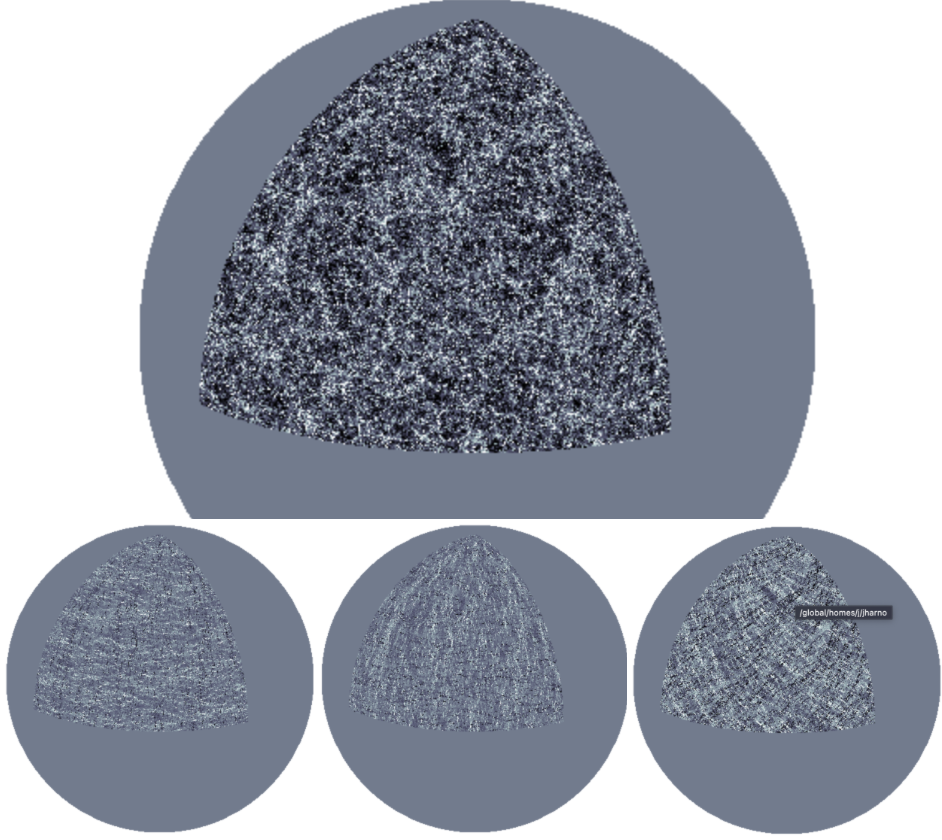
\includegraphics[width=\columnwidth]{graphs/TidalFieldOuterRim_V0}
\caption{Density field (top)  and the associated projected tidal field tensors $s_{11}$, $s_{22}$ and $s_{12}$, from left to right ({\it Improve this figure...}).}
\label{fig:maps}
\end{figure}



Our infusion method relies on couplings between intrinsic galaxy shapes and the local tidal field, hence the first step in our method consist in extracting the tidal field maps $s_{ij}(\theta,\phi)$ from the mass maps $\delta(\theta,\phi)$ that source them\footnote{Note that we have removed the redshift indexing of the maps here to simplify notation, {\it i.e.} $\delta_i(\theta,\phi) \rightarrow \delta(\theta,\phi)$.}.
In three dimensions, trace-free tidal tensor $s_{ij}(\boldsymbol x)$ can be obtained from the matter over-density field $\delta(\boldsymbol x)$ as   \citep{Catelan_IA_Tidal}:
\begin{eqnarray}
 \widetilde{s}_{ij} (\boldsymbol k)  = \left[\frac{k_i k_j}{k^2} - \frac{\delta_{ij}}{3}\right]  \widetilde {\delta}(\boldsymbol k) \mathcal{G}(\sigma_{\rm G}) \, ,
 \label{eq:sij}
\end{eqnarray}
where $\mathcal{G}(\sigma_{\rm G})$ is a three-dimensional Gaussian function described by a single (free) parameter $\sigma_{\rm G}$ that  controls the physical scales which are allowed to affect the IA term in our model. 
Tilde symbols denote Fourier-transformed quantities, the indices $(i,j)$ label the components of the Cartesian wave-vector $\boldsymbol{k}^T = (k_1,k_2,k_3)$, and $k^2 = k_1^2 + k_2^2 + k_3^2$. 
As shown in \citet{Tidalator} in the flat-sky approximation, projected tidal fields  computed from projected mass sheets provide and excellent agreement with the  theoretical NLA model, which in contrast computes the full tidal fields from the three-dimensional matter density and project along the radial dimension at the end.
We promote here this transformation to curved-sky maps, exploiting the  polarisation {\sc alm2map} operations built in {\sc Healpy}. 
In particular, noting that $Q=s_{11}-s_{22}$, $U=s_{12}$, and $\delta=s_{11}+s_{22}$, we compute the curved-sky projected  tidal field tensors ${s}_{ij}({\boldsymbol \theta})$ as:
\begin{equation}\label{eq:sij_2D_sph}
\begin{split}
    s_{11}({\boldsymbol \theta})  &=  \frac{1}{\Delta \chi_{\rm shell}}\left[\frac{ \delta + Q}{2}  - \frac{\delta}{3}\right] \\ s_{22}({\boldsymbol \theta})  &=   \frac{1}{\Delta \chi_{\rm shell}}\left[\frac{\delta - Q}{2}  - \frac{\delta}{3}\right] \\ s_{12}({\boldsymbol \theta}) &=  \frac{U}{\Delta \chi_{\rm shell}} 
\end{split}
\end{equation}
where the $U({\boldsymbol \theta})$ and $Q({\boldsymbol \theta})$ maps are smoothed by the Gaussian beam with width $\sigma_{\rm G}$, and the normalisation by  $\Delta \chi_{\rm shell}$ is required to account for the comoving thickness of the shells.
We suppress large artificial tidal fields at the boundary of our simulated octant by replicating 8$\times$ the  $\delta$ maps and carrying out these harmonic calculations  on full sky densities; we re-apply the octant mask on the tidal field maps after the last operation.
Note that the value of $\sigma_{\rm G}$ is a free parameter both in the infusion technique described in this paper and in the NLA and TATT models.
We therefore explore two cases, $\sigma_{\rm G}=0.1\mathrm{Mpc}$ and $0.5\mathrm{Mpc}$, however this may be further optimised in the future.
Finally, the full-sky density field is downgraded from $N_{\rm side}=8192$ to $N_{\rm side}=4096$ since the smoothing washes the smallest angular scales. 


%are specified within the NLA model. Smoothing amounts to selecting physical scales that do not contribute to the alignment of galaxies, which is still a debatable quantity, but is also introduced for numerical stability. \citet{Blazek2015} argues that 1.0 $h^{-1}$Mpc could be a reasonable fiducial value, being larger then the typical halo size, but recognizes that one-halo terms are also required to better match the observations. In their later work, \citet{Blazek2019} do not include smoothing at all, and neither do the KiDS-1000 nor DES-Y1 analyses based on the NLA model \citep{KiDS1000_Asgari,DESY1_Troxel}. In this work we used a two-dimensional Gaussian filter and calibrated $\sigma_{\rm G}$ empirically to $\sigma_{\rm G}=0.1h^{-1}$Mpc (see Sec. \ref{subsubsec:sigma_G}), however these two choices are arbitrary and could possibly be better optimised in the future; we also explore $\sigma_{\rm G}=0.5h^{-1}$Mpc later on.  We note that the smoothing scale is degenerate with the resolution of the simulation itself, and that one should use caution when smoothing on scales that approach the resolution limits.

%We employ a numerical technique worth mentioning here: the Fourier transforms involved in computing Eq. (\ref{eq:sij_2D}) are computed from the full (projected) periodic boxes of the simulations, then interpolated on the light-cones. We find that tidal field computed directly from the $10\times10$ deg$^2$ light-cones introduces significant large scales features in the tidal field maps, largely caused by  the non-periodic boundary conditions, which our method avoids.
Projected tidal field maps $s_{11}$, $s_{22}$, and $s_{12}$ are constructed that way for each mass sheets; Fig. \ref{fig:maps} shows the  three tidal fields and the underlying density maps for one of them.
We can clearly see the connection between all maps around over-dense regions. . 


%of every light-cones and interpolated at the position of every galaxy. Fig. \ref{fig:tidalator} illustrates this process for a small zoomed-in patch at $z\sim0$, starting from a $\delta_{2D}(\boldsymbol \theta)$ map (upper large panel), computing the tidal field components (middle four panels) and comparing the results with the cosmic shear signal generated by the same mass distribution (bottom two panels). The tidal field maps clearly reproduce the cosmic shear maps, and the minus sign in front of both terms in Eq. (\ref{eq:tidal_th}) causes the IA to undo some of the lensing signal.

\subsection{Infusion of intrinsic alignments}
\label{subsec:IA_infusion}

Having now produced shear catalogues and tidal field maps, we can use Eq. (\ref{eq:tidal_th}) to couple linearly the alignment of galaxies with the local tidal field, or Eq. (\ref{eq:tidal_th_TT}) to use instead a quadratic coupling. These allow us to compute the intrinsic ellipticities ${\boldsymbol \epsilon}^{\rm int}$ for the six IA models described in Sec. \ref{sec:IA_th}, which we combine with the cosmic shear signal ${\boldsymbol g}$ to compute observed ellipticities: 
\begin{equation}
{\boldsymbol \epsilon}^{\rm obs} = \frac{{\boldsymbol \epsilon}^{\rm int} + {\boldsymbol g}}{1 + {\boldsymbol \epsilon}^{\rm int}{\boldsymbol g^*}} 
\label{eq:eps_obs}
\end{equation}
with
\begin{equation}
{\boldsymbol \epsilon}^{\rm int}  = \frac{{\boldsymbol \epsilon}^{\rm IA} + {\boldsymbol \epsilon}^{\rm ran}}{1 + {\boldsymbol \epsilon}^{\rm IA}{\boldsymbol \epsilon^{\rm ran, *}}}.
\label{eq:eps_int}
\end{equation}
In the above expressions, the denominators ensure that the combined  ellipticities never exceed unity.
The complex spin-2 reduced shear
\begin{equation}
{\boldsymbol g} \equiv \frac{\gamma_1 + {\rm i} \gamma_2}{1 + \kappa}
\end{equation}
is computed from the shear  $(\gamma_{1/2}$) and convergence ($\kappa$) maps, interpolated at the galaxy positions and redshifts. 
The random orientation term ${\boldsymbol \epsilon}^{\rm ran}$ is drawn from two Gaussians (one per component\footnote{We further constraint  the random ellipticity to satisfy $|{\boldsymbol \epsilon}^{\rm ran}| \le 1.0$.}) with their standard deviations matching the LSST-Y1 forecast, $\sigma_{\epsilon} = 0.27$, although in most calculations we work with noise-free shapes to better resolve the IA signal.  
%We recall that since our simulated galaxy catalogues trace the dark matter density, our default IA-infusion method  is consistent with the $\delta$-NLA model (see Sec. \ref{subsec:IA_th_ext}). Analytical predictions for the two-point functions are more involved in this case \citep[see][]{Blazek2019} and not yet available on the public {\sc cosmoSIS} release. We therefore validate our methods with the standard NLA first, which we infuse by `correcting' the $\delta$-NLA measurement with Eq. (\ref{eq:tidal_th_deltaNLA}), i.e. by replacing ${\boldsymbol \epsilon}^{\rm IA}$ by ${\boldsymbol \epsilon}^{\rm IA}/(1 + b_{\rm TA} \delta)$ in our simulations. Once again, these are less realistic but better suited for validation of the measured $\gamma$-2PCFs against a theoretical model; after this is established, we use the $\delta-$NLA catalogues as our fiducial infusion model. 
%We re-iterate here that the same tidal fields, shear maps, and IA coupling equations are used for the NLA and \dNLA models, and separately for the TT and \dTT models; these only differ by the fact that in one case the galaxies are placed at random on the octant, while in the other case they are linearly tracing the dark matter.
Finally, once all galaxies have been placed in the light-cone, we interpolate the shear and IA quantities at their exact location.
Note that our current IA models make no differentiation between galaxy colours or type, and instead treats the full sample as a single population that has a single, effective, alignment signal \citep[see][for an example with a red/blue split]{DESY1_IA_Samuroff}.



\section{Validation with $\xi_{\pm}$}
\label{sec:validation}



This section presents a comparison between theoretical predictions and measurements in the simulations for all our 6 models. We include here the statistical error obtained from covariance matrix computed analytically as described in \citet{KiDS1000_Joachimi}, which includes contributions from the Gaussian, non-Gaussian and super-sample covariance terms, assuming survey properties that match our simulation in terms of area, shape noise, galaxy density, tomographic $n(z)$ and cosmology.   The diagonal elements are used to assign the error bars in our figures, and the full matrix is used in the MCMC analyses presented in Sec. \ref{sec:inference}.

%---------------
\begin{figure*}
%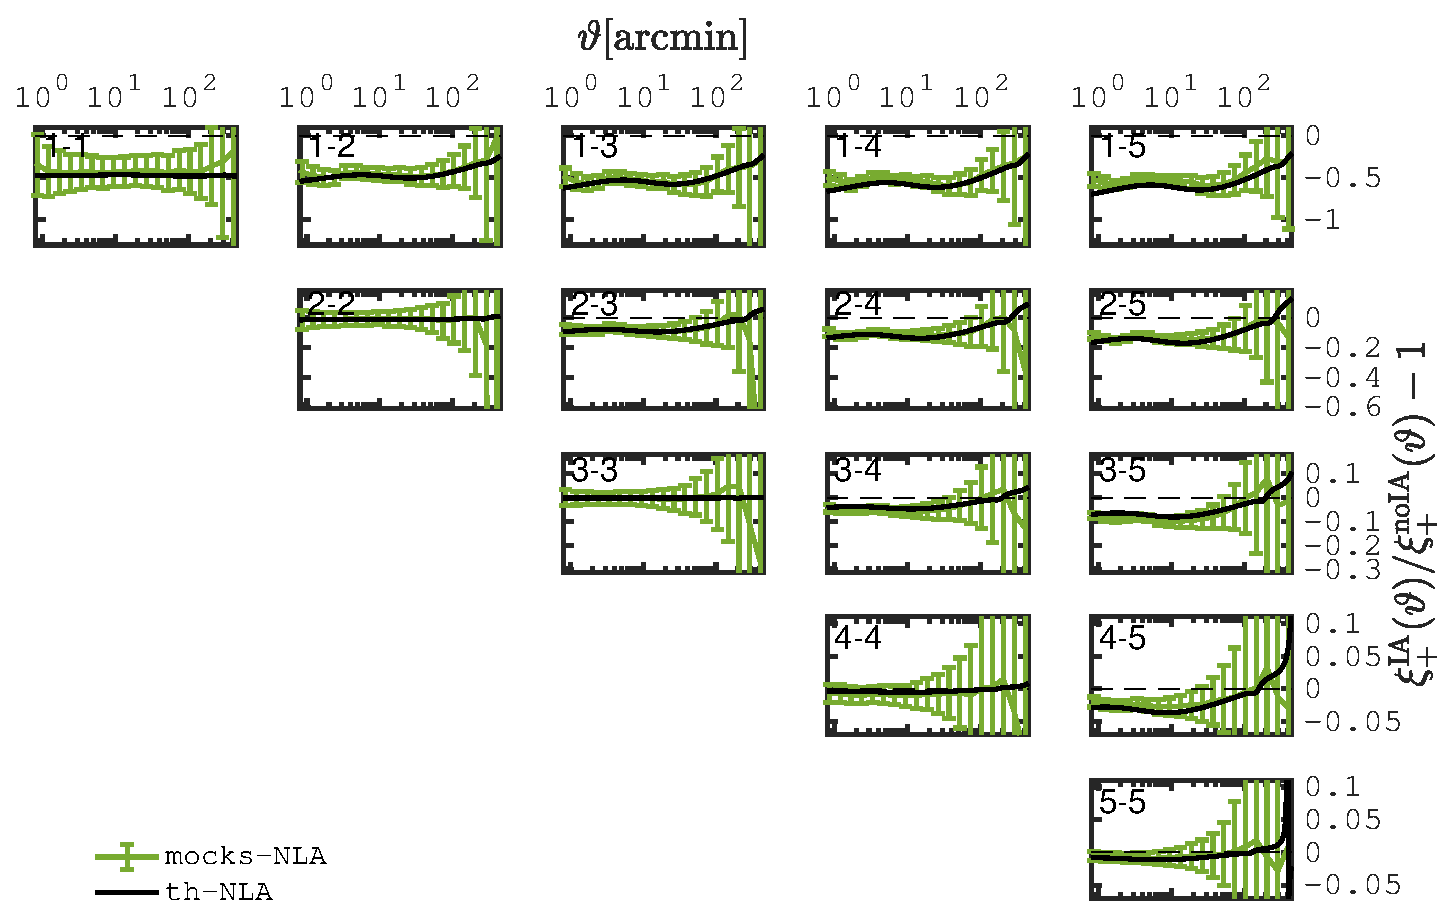
\includegraphics[width=\columnwidth]{graphs/frac_xip_IA1_skysim}
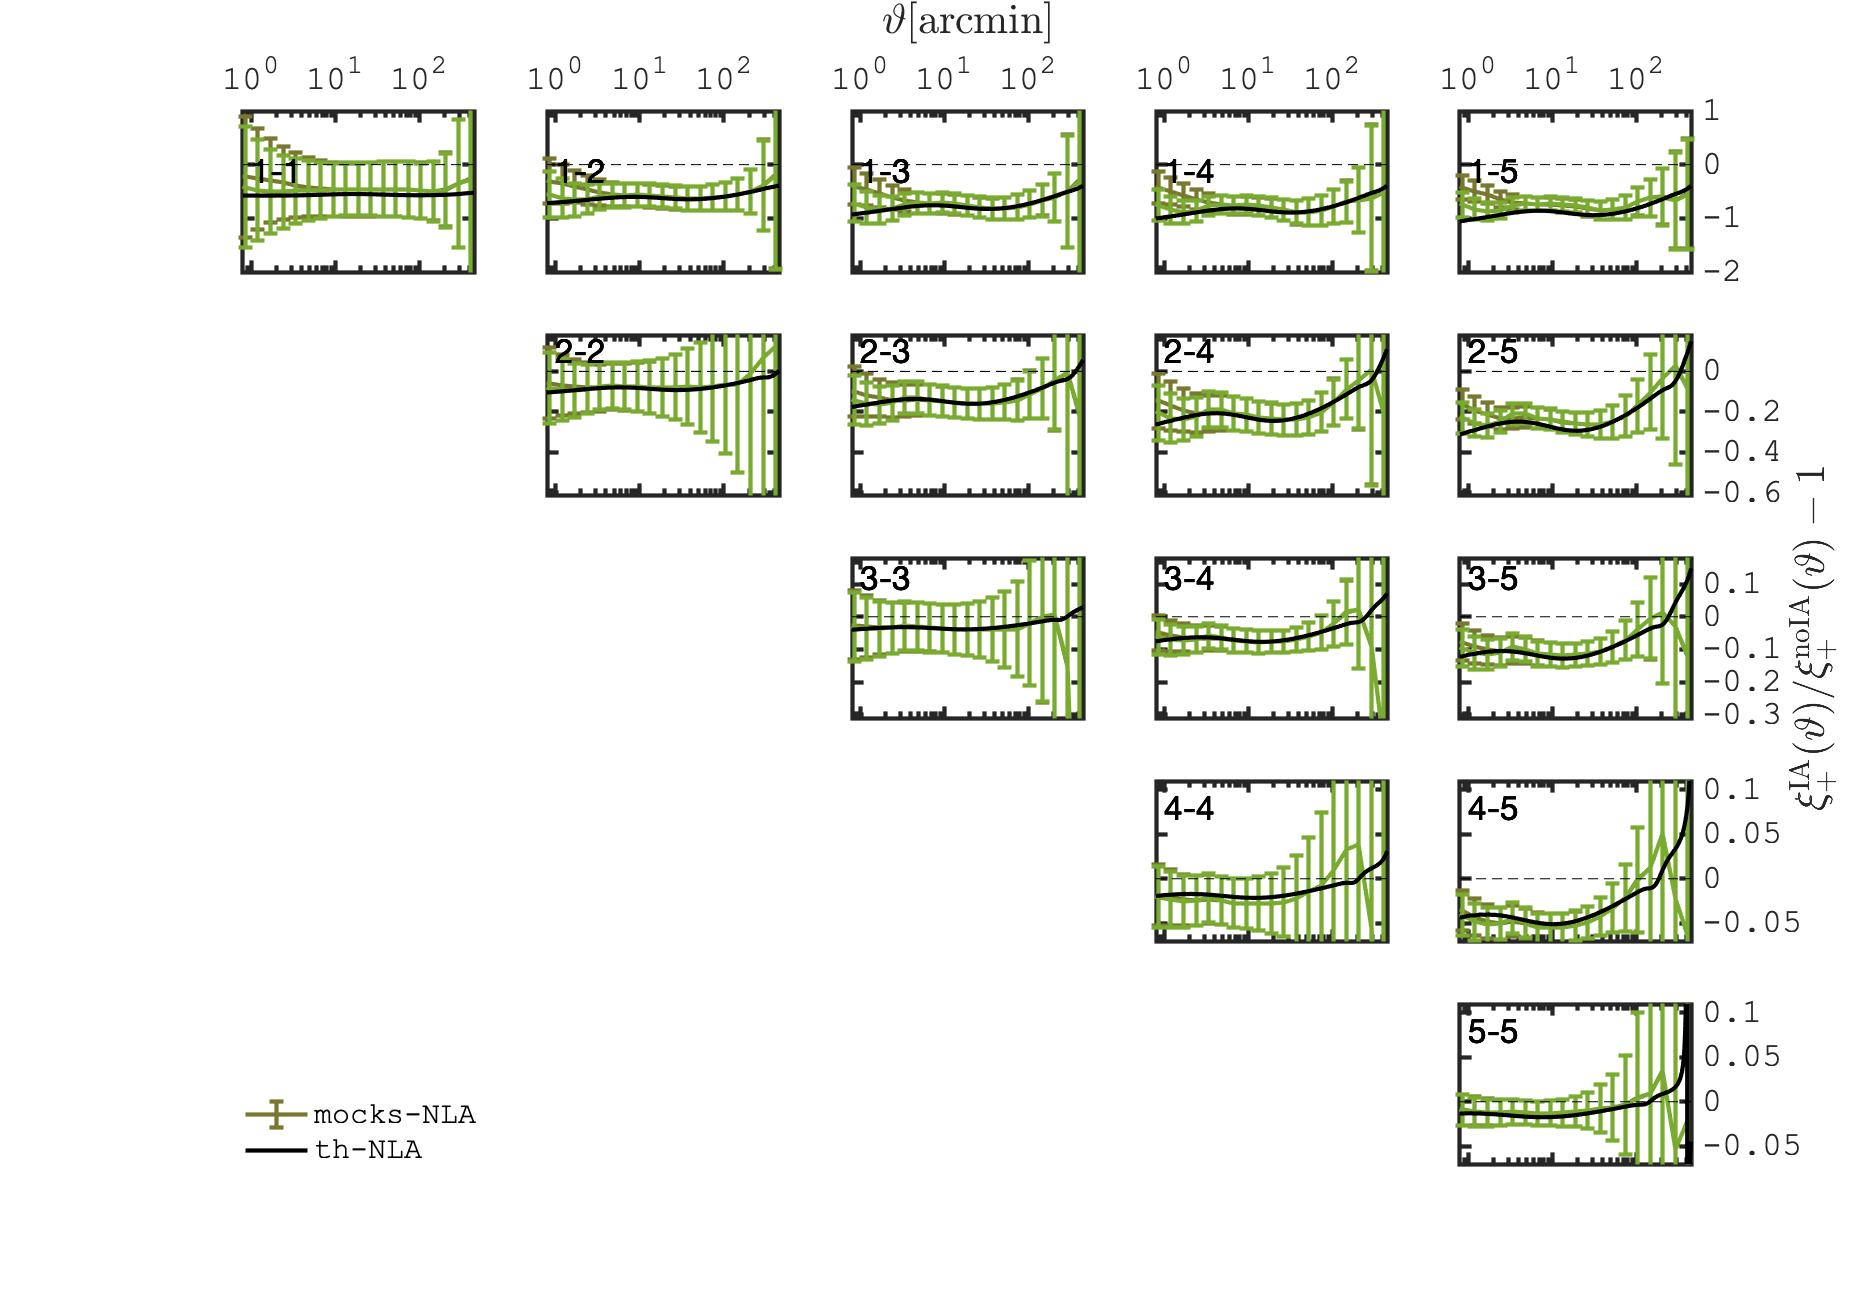
\includegraphics[width=\columnwidth]{graphs/frac_xip_IA1_skysim_NLA_srd.jpg}
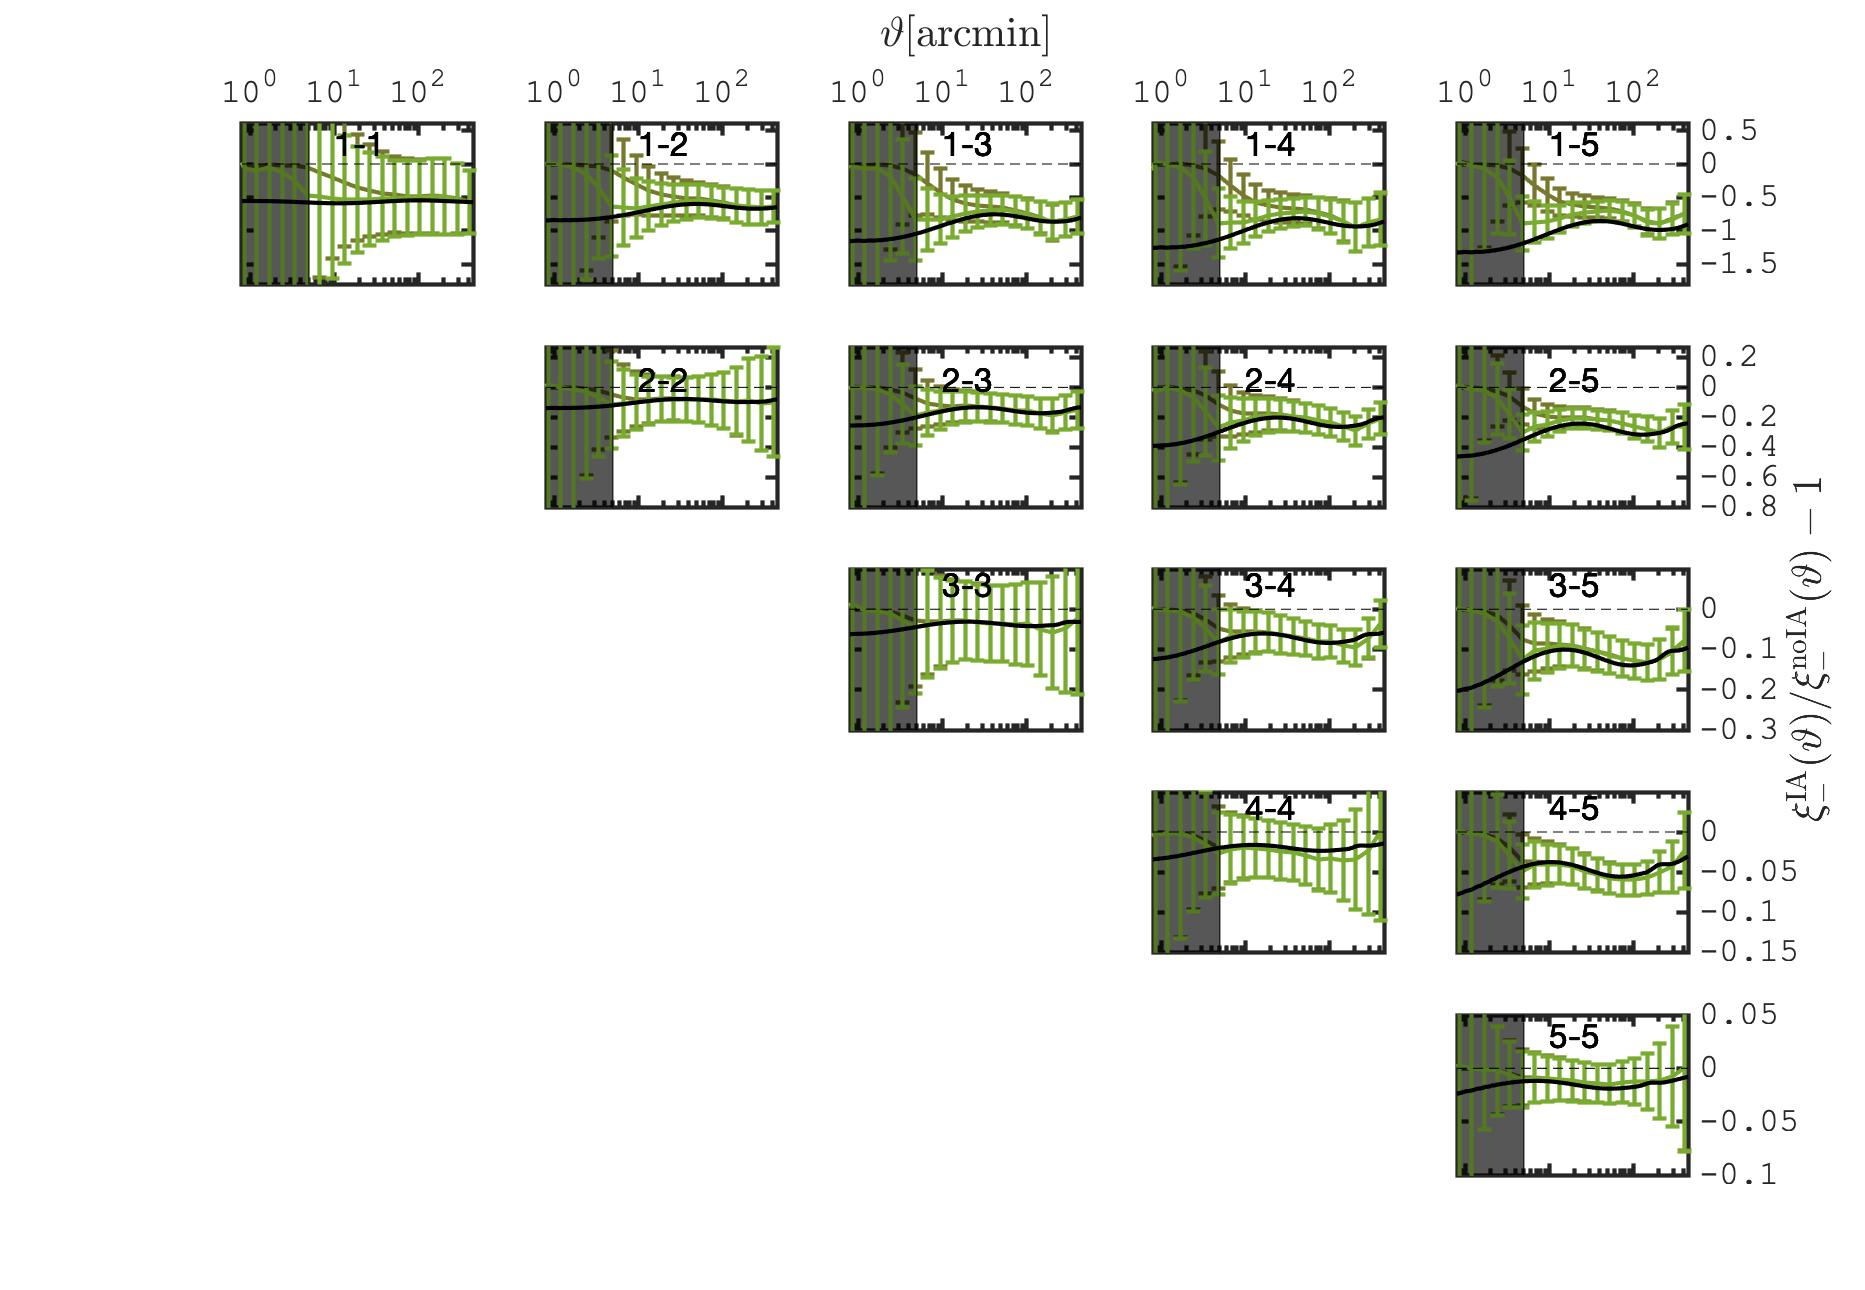
\includegraphics[width=\columnwidth]{graphs/frac_xim_IA1_skysim_NLA_srd.jpg}
\caption{Ratio between the shear correlation functions with and without IA, assuming the NLA model with $A_{\rm IA}=1.0$ both in the simulations and theory. Measurements shown in green and brown correspond to smoothing scales of 0.1 and 0.5 $h^{-1}$Mpc in the tidal field. There is no shape noise in the simulations, but it is included in the error bars.}
\label{fig:xi_NLA}
\end{figure*}
%---------------


\subsection{Data vector}
%------------------------------
\subsubsection*{NLA model}

We start by presenting a comparison between the relative impact of IA in the NLA model as measured in the simulations and as modelled by {\sc cosmoSIS}. Specifically, we show in Fig. \ref{fig:xi_NLA} the ratio between the $\gamma$-2PCF with and without IA, for all combinations of tomographic bins as indicated in the panels, and for two smoothing scales. The agreement is remarkable over all scales except for the smallest angular separations in $\xi_-$, where deviations are weaker in the simulations due to limits in the resolution.  The grey bands  indicates scales that are not well modelled and should be avoided, set to 5 arcmin. The smaller smoothing scales shows better agreement with the model at the smallest angular scales. 


%------------------------------
\subsubsection*{Extended-NLA model}
\begin{figure*}
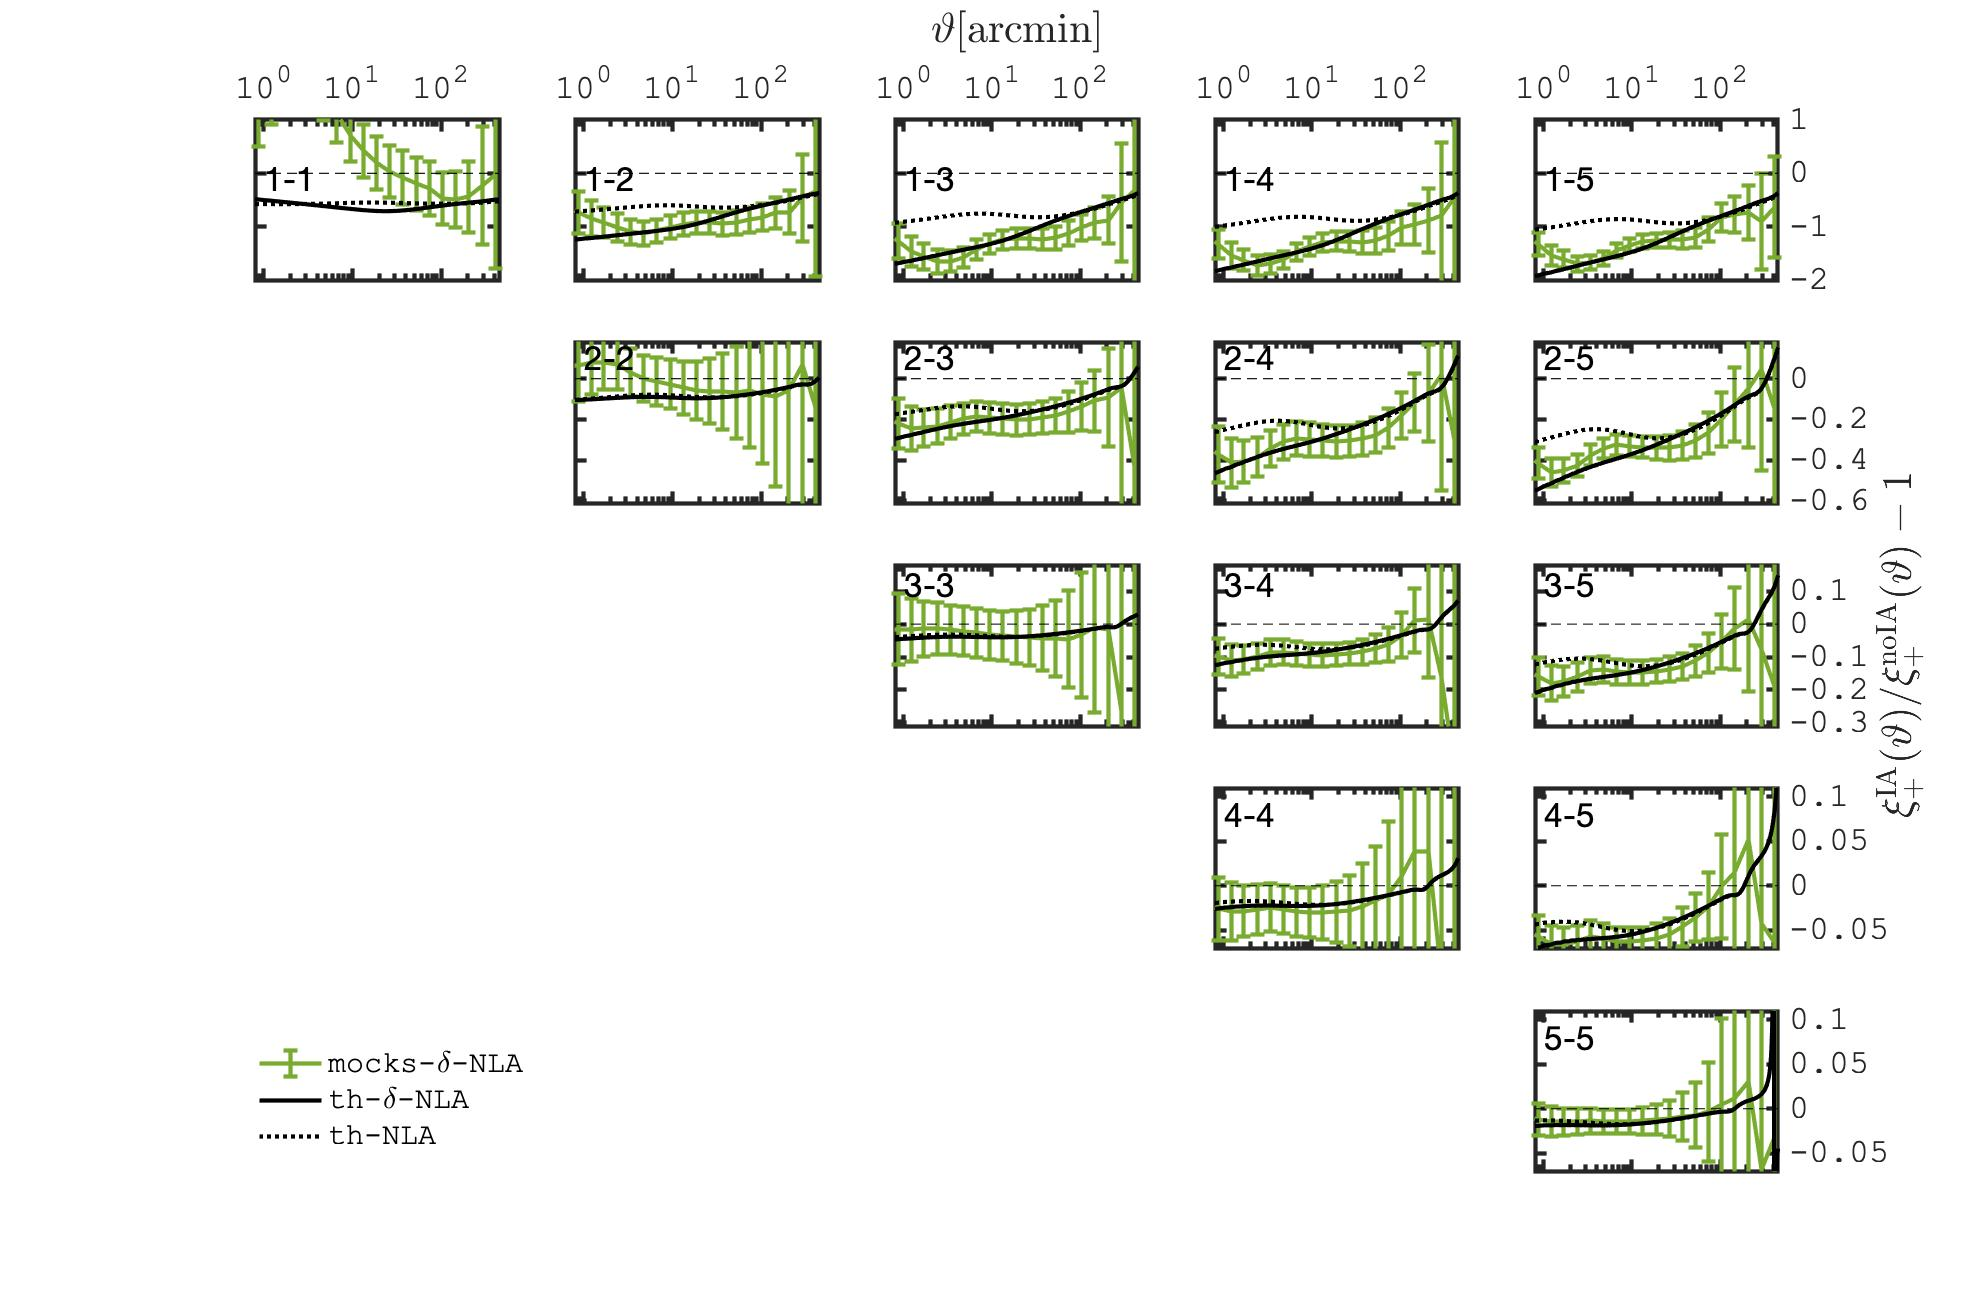
\includegraphics[width=\columnwidth]{graphs/frac_xip_IA1_skysim_deltaNLA_srd}
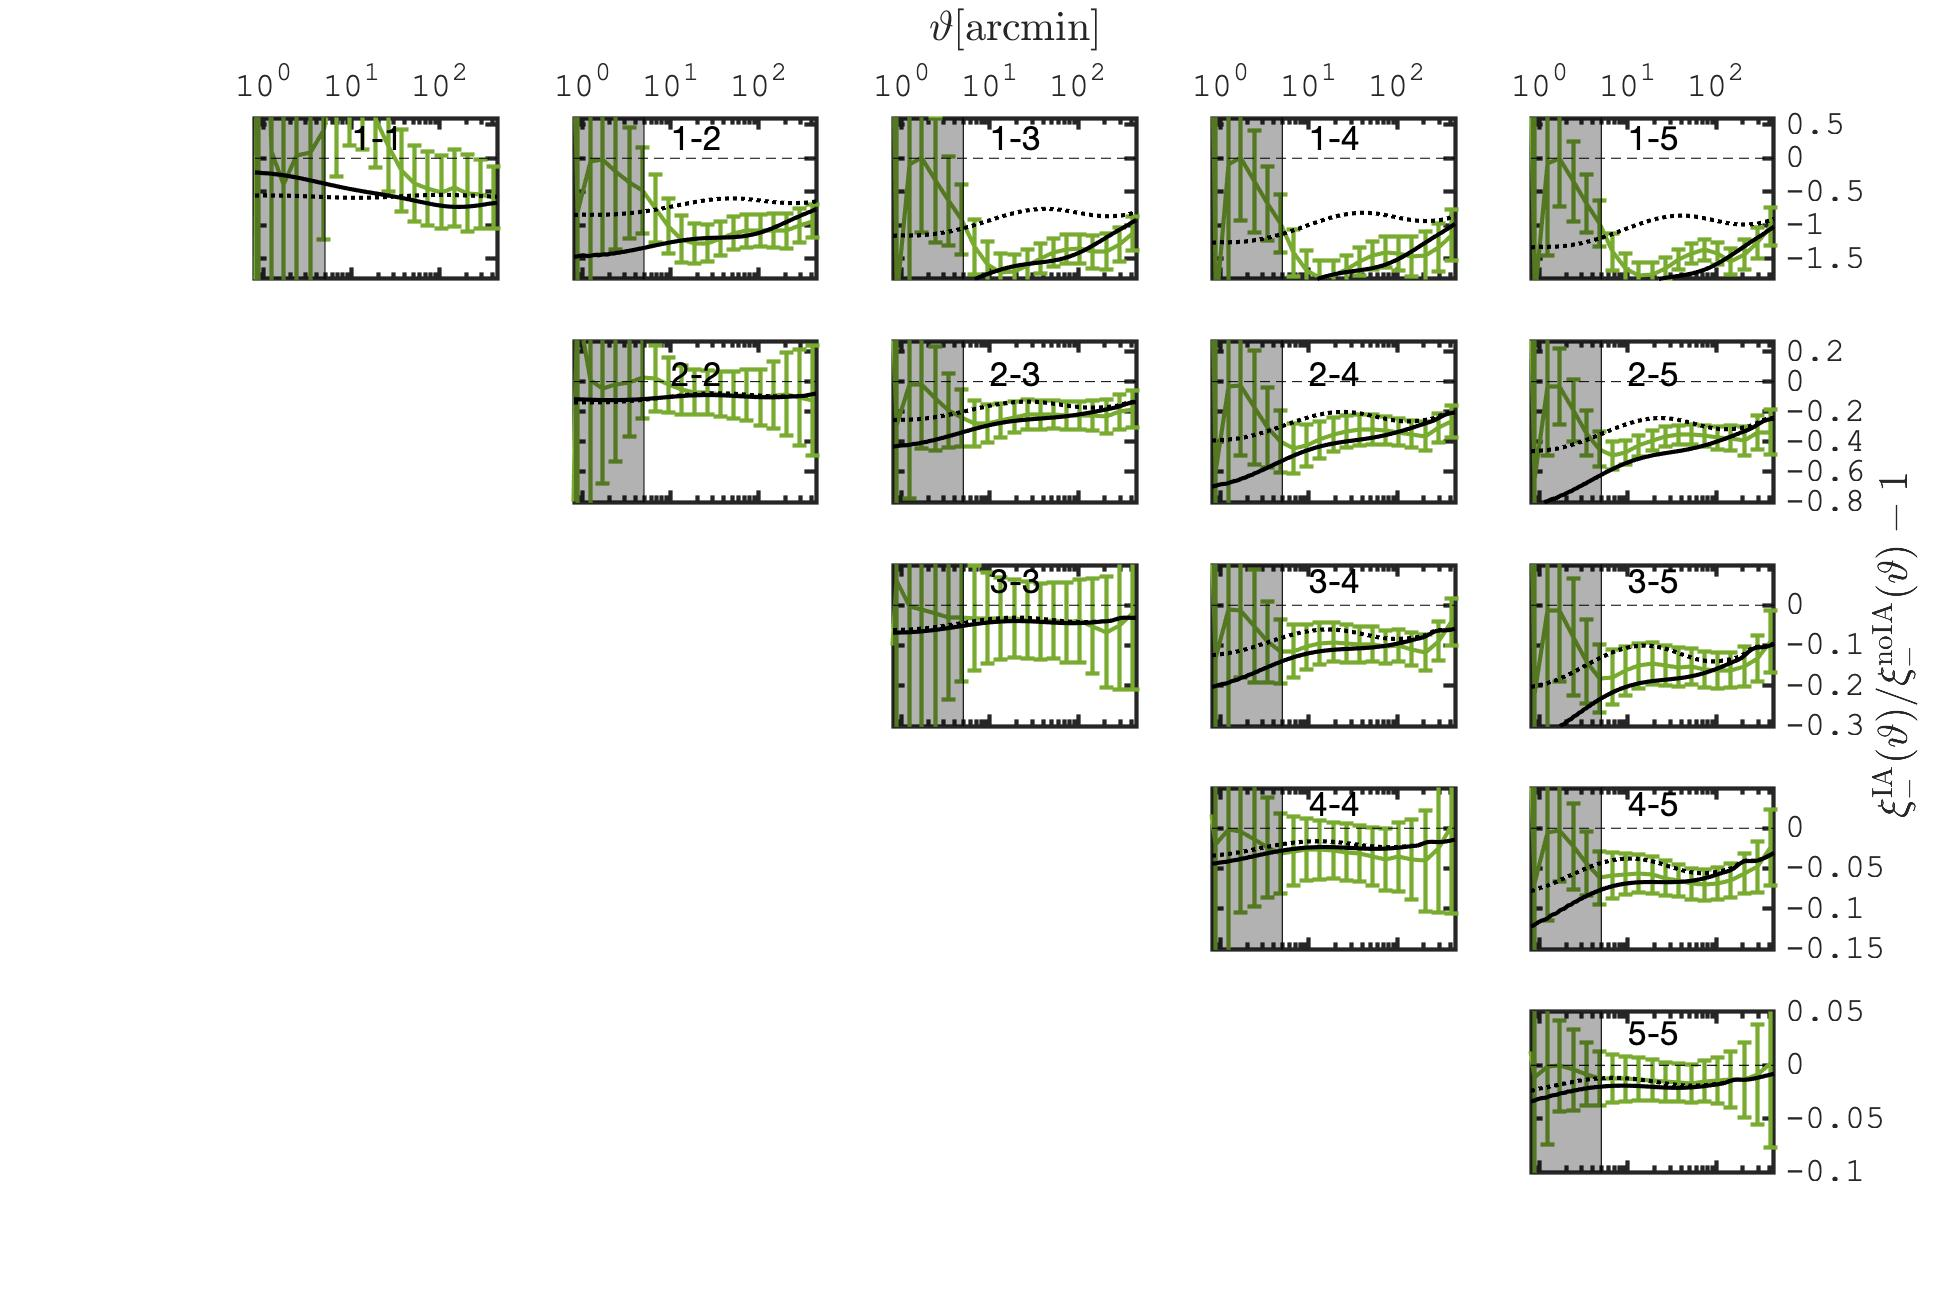
\includegraphics[width=\columnwidth]{graphs/frac_xim_IA1_skysim_deltaNLA_srd}
\caption{Same as Fig. \ref{fig:xi_NLA}, but for the $\delta$-NLA model with $A_{\rm IA}=1.0$ and $b_{\rm TA}=1.0$, and only for smoothing of 0.5$h^{-1}$Mpc. The dashed black lines show the NLA predictions to better highlight the differences.  }
\label{fig:xi_deltaNLA}
\end{figure*}

\begin{figure}
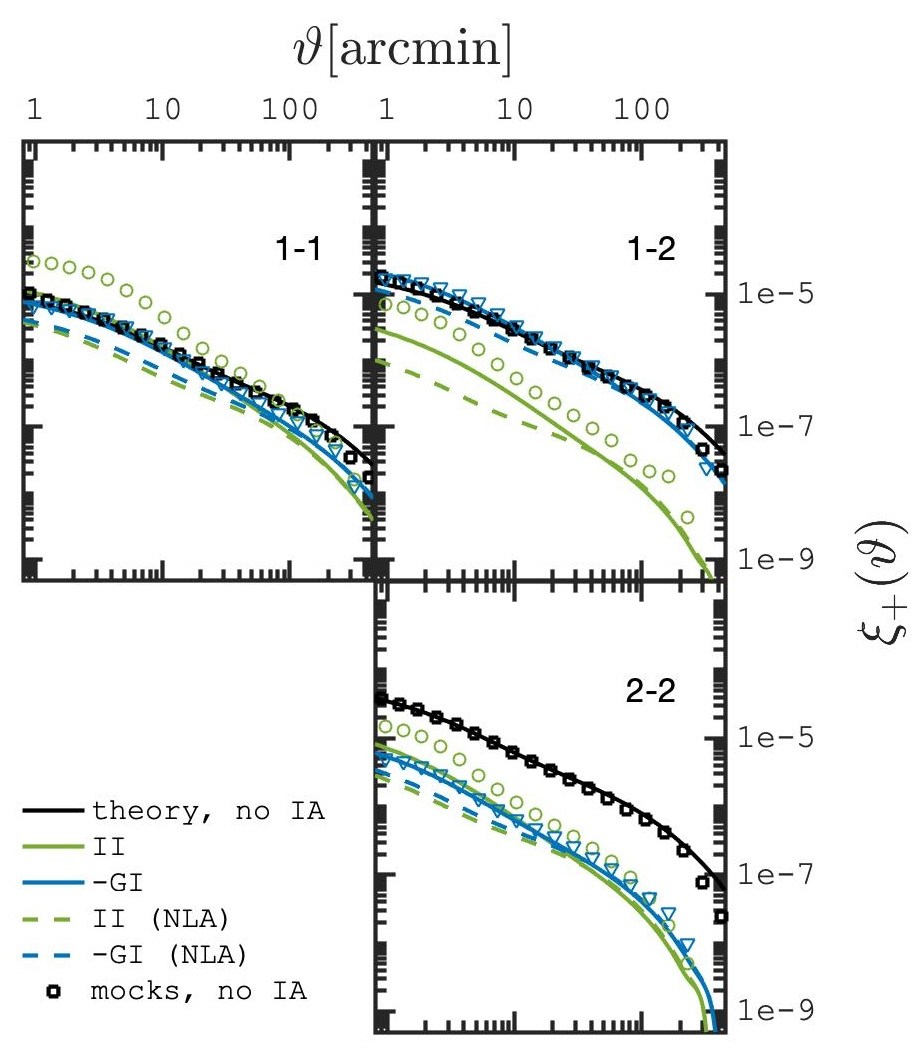
\includegraphics[width=\columnwidth]{graphs/xip_deltaNLA_bta1}
\caption{Shear 2PCF in the extended-NLA model for the two lowest redshift bins, showing the good agreement between simulations and theory for the $GG$ (black) and $GI$ (blue) terms, and large deviations in the $II$ term (green). {\it (Re-do legend)}}
\label{fig:xi_deltaNLA_II}
\end{figure}

\begin{figure}
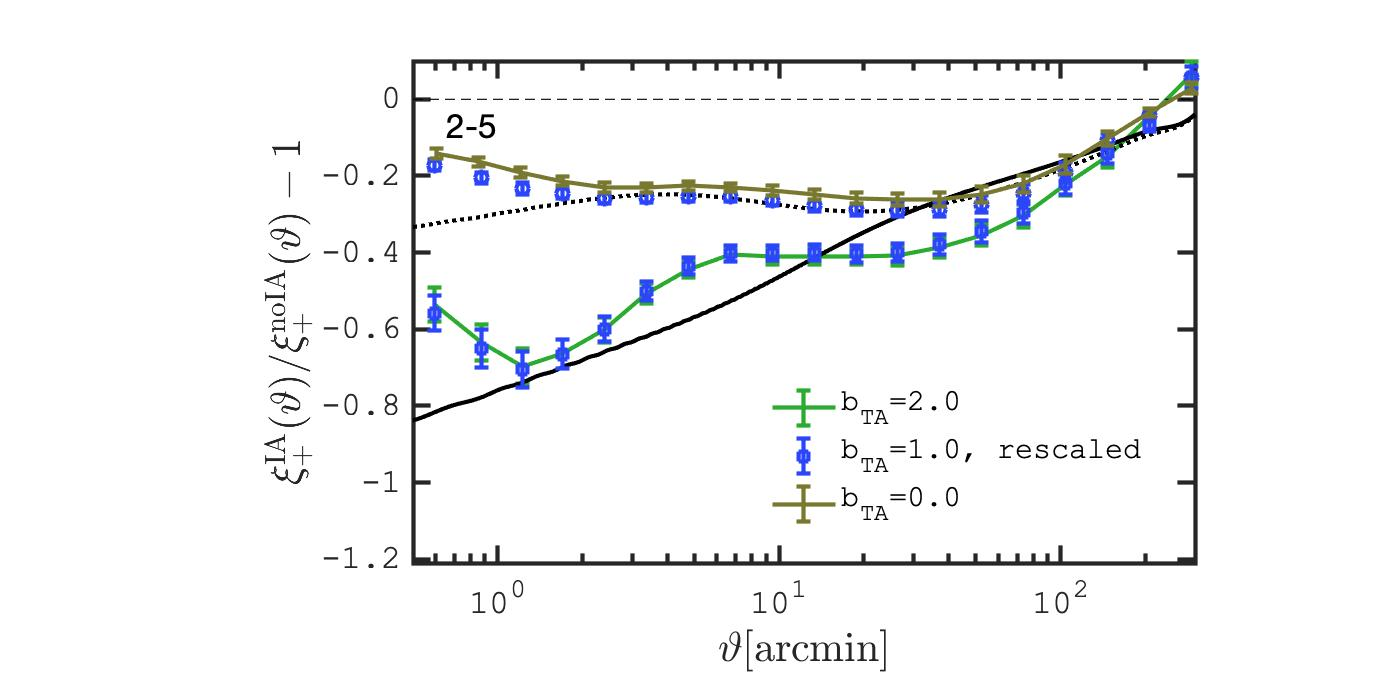
\includegraphics[width=\columnwidth]{graphs/frac_xip_bta1_rescaled}
\caption{Ratio between the shear correlation functions with and without IA in tomographic bin combination 2-5.
The brown and green symbols show measurements from simulations constructed with $b_{\rm TA}$ = 0.0 and 2.0 respectively,  the black solid and dotted lines shown their predictions, while the blue symbols are obtained by rescaling $b_{\rm TA}$ = 1.0 simulations using Eq. \ref{eq:bta_rescale}.  }
\label{fig:xi_deltaNLA_rescaled}
\end{figure}

The equivalent comparison for the extended-NLA model is presented in Fig. \ref{fig:xi_deltaNLA}, where we also find an excellent match with the theoretical predictions except for redshift bins 1-1 and 2-2, where the $II$ term is important and much larger in the simulations than in the theory. This is expected since the former includes additional terms that are up to second order in perturbation theory. This is shown in Fig. \ref{fig:xi_deltaNLA_II}, where the different contributions are separated, clearly showing the disagreement in  the $II$ term. 

The results are shown here for $b_{\rm TA}$ = 1.0  and we verified that it works equally well for $b_{\rm TA}$ =  2.0. Using the former, we test the $b_{\rm TA}$-rescaling method introduced in Eq. \ref{eq:bta_rescale} to generate $b_{\rm TA}=2.0$ and $b_{\rm TA}=0.0$ mocks, and compare the outcome with mocks constructed directly with these bias values. Results are shown in Fig. \ref{fig:xi_deltaNLA_rescaled} for one of the tomographic bins for which IA has the strongest effect. The match is excellent here, however lower redshift are less accurate due to the increased shot noise (not shown){\it (should I show an example?)}, hence we recommend producing new mocks over using this rescaling method whenever possible. 

Note that since source clustering is a higher order effect in cosmic shear, the measured $\xi_{\pm}$ from mocks with $b_{\rm TA}$=0.0, 1.0 and 2.0 show negligible differences in $\xi_+$, and becomes detectable only at the smallest scales  (i.e. $\vartheta<5$arcmin) in $\xi_-$, consistent with  \citet{source_lens_clustering} who find an effect of a few percent for $\ell>3000$, and with \citet{DESY3_Gatti_source_clust}, who find minor impact for second moments of aperture mass maps. However the impact on higher order lensing statistics and on the overall  IA contamination is significant and can double the secondary signal in certain circumstances, due to the up-sampling of regions with strong tidal forces. 

% Requires the booktabs if the memoir class is not being used
\begin{table}
   \centering
   %\topcaption{Table captions are better up top} % requires the topcapt package
    \caption{IA models infused in this work and the respective fiducial values of the model parameters.}
   \begin{tabular}{@{} lcr @{}} % Column formatting, @{} suppresses leading/trailing space
      \hline
      \hline
      %\multicolumn{2}{c}{Item} \\
      model   		& ($A_{\rm IA}, \: b_{\rm TA}, \: A_2)$ \\
      \hline
      NLA     		& ($\pm$1, 0, 0) &  \\
      \hline
      \multirow{2}{*}{extended-NLA }  	&   ($\pm$1, 1, 0)   \\
                                        &  (1, 2, 0)   \\
      \hline
      TT 			&  {(0, 0, $\pm$1)} &  \\
      \hline
      \multirow{2}{*}{extended-TT} 	    &  (0, 1 ,$\pm$1)   \\
                                        &  (0, 2, 1)   \\
      \hline
      TATT- fiducial	&  (1, 1, 1)  \\
      \hline
      \hline
   \end{tabular}
   \label{table:IAmodels}
\end{table}





%------------------------------


%------------------------------
\subsubsection*{TT model}
\label{subsec:TT}

Results for the tidal torque model are presented in Fig. \ref{fig:xi_TT}, again for two smoothing scales. In this case, we see that the larger smoothing scales agrees better with the theoretical predictions, likely due a mis-matched caused by projection effects. Indeed, the TT model, being quadratic in the tidal field, is more sensitive to smaller scales \citep{TATT}, and the missing third dimension inherent to our method is more prone to cause inaccuracies. We observe discrepancies in the small angular separations for  $\xi_-$ at low redshifts, but achieve better match for $\vartheta>$  40 arcmin.

Importantly, we found that our implementation of the TT model yields alignments that are too strong at low redshifts, and hence requires an empirical redshift-dependent calibration to improve the match with theory. We achieve this by rescaling $\epsilon^{\rm IA, TT}(z<0.5) \rightarrow \epsilon^{\rm IA, TT} /2.5$, acknowledging that this exhibits limits in our capacity to model the tidal torquing without accessing the third dimensional of the tidal field. 

\begin{figure*}
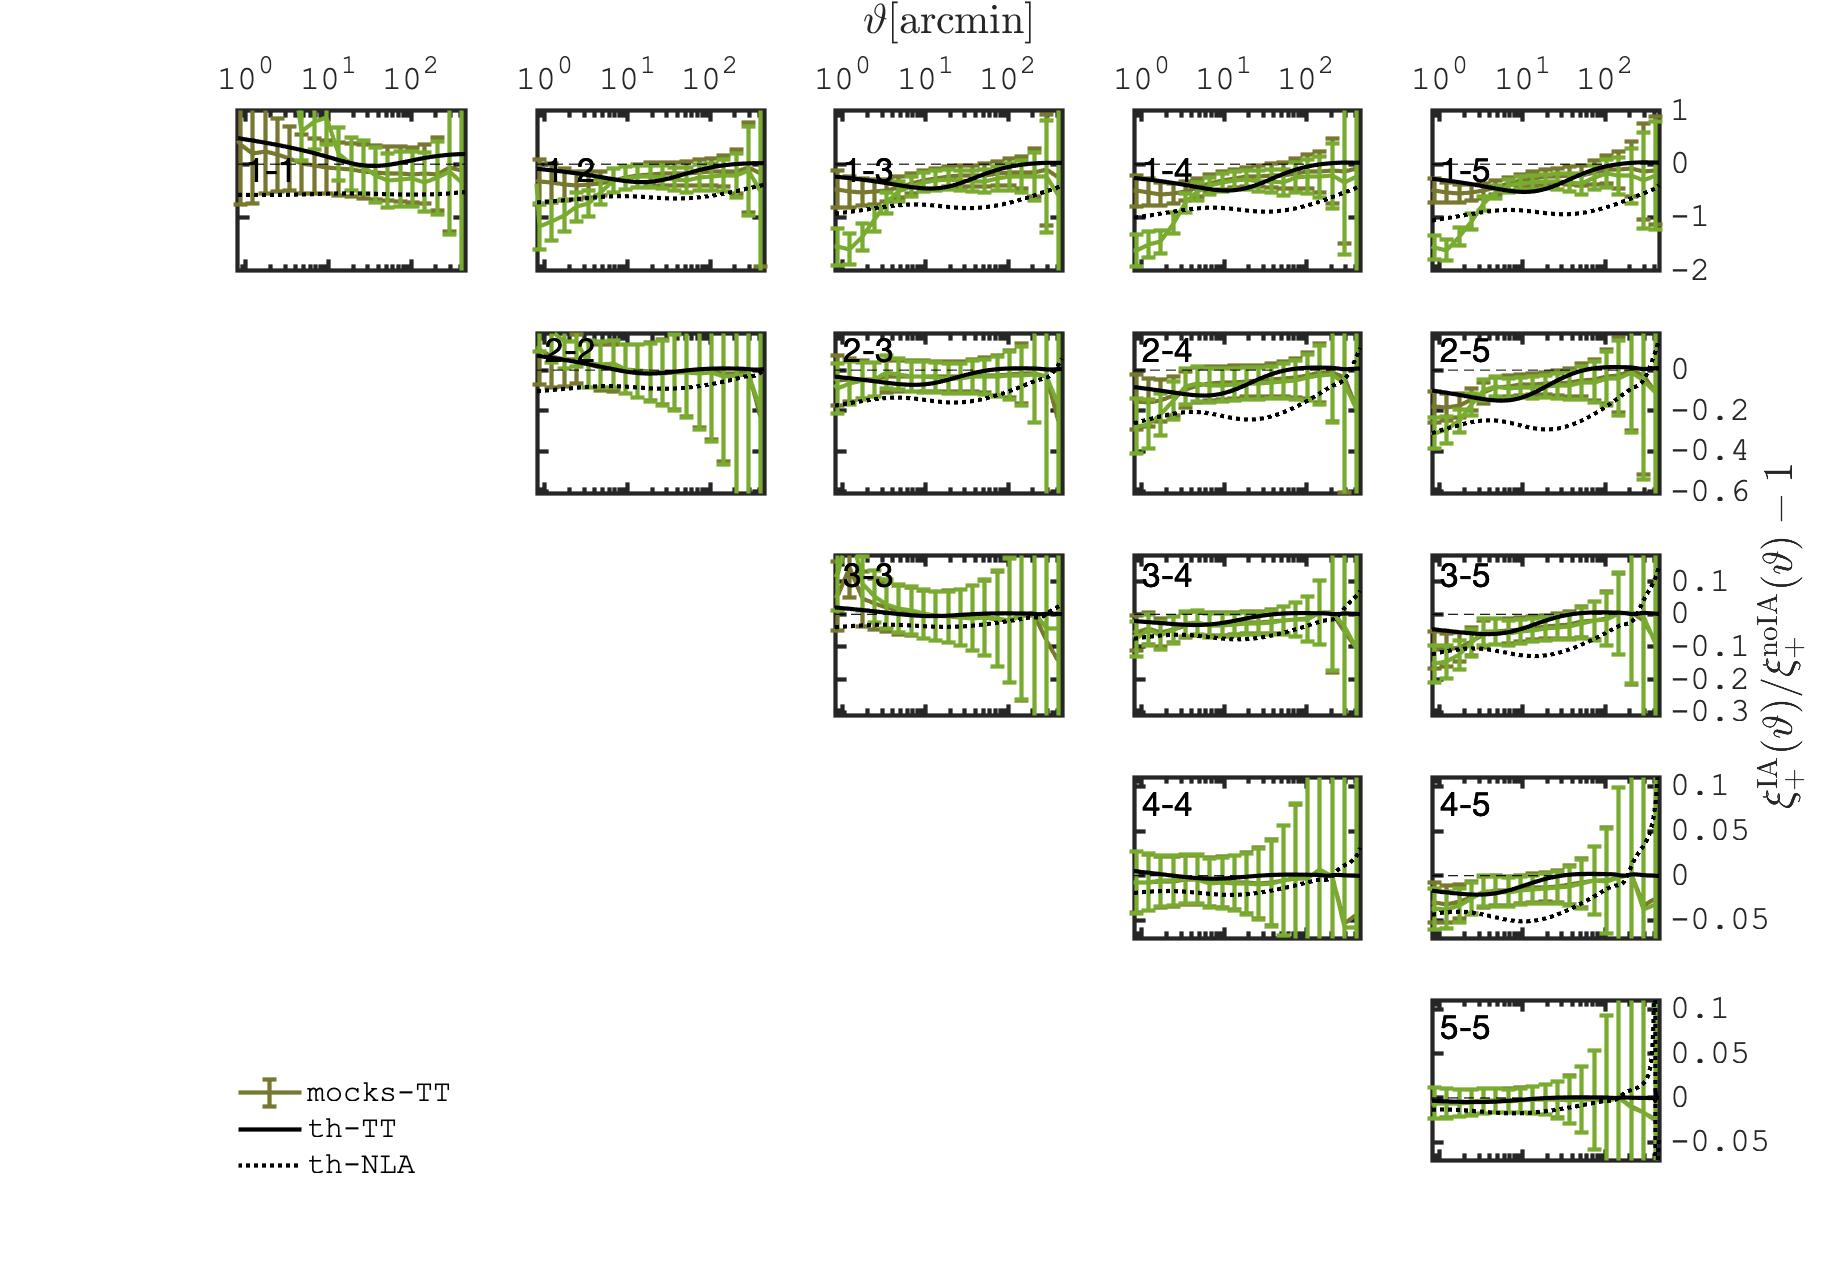
\includegraphics[width=\columnwidth]{graphs/frac_xip_IA1_skysim_TT_srd.jpg}
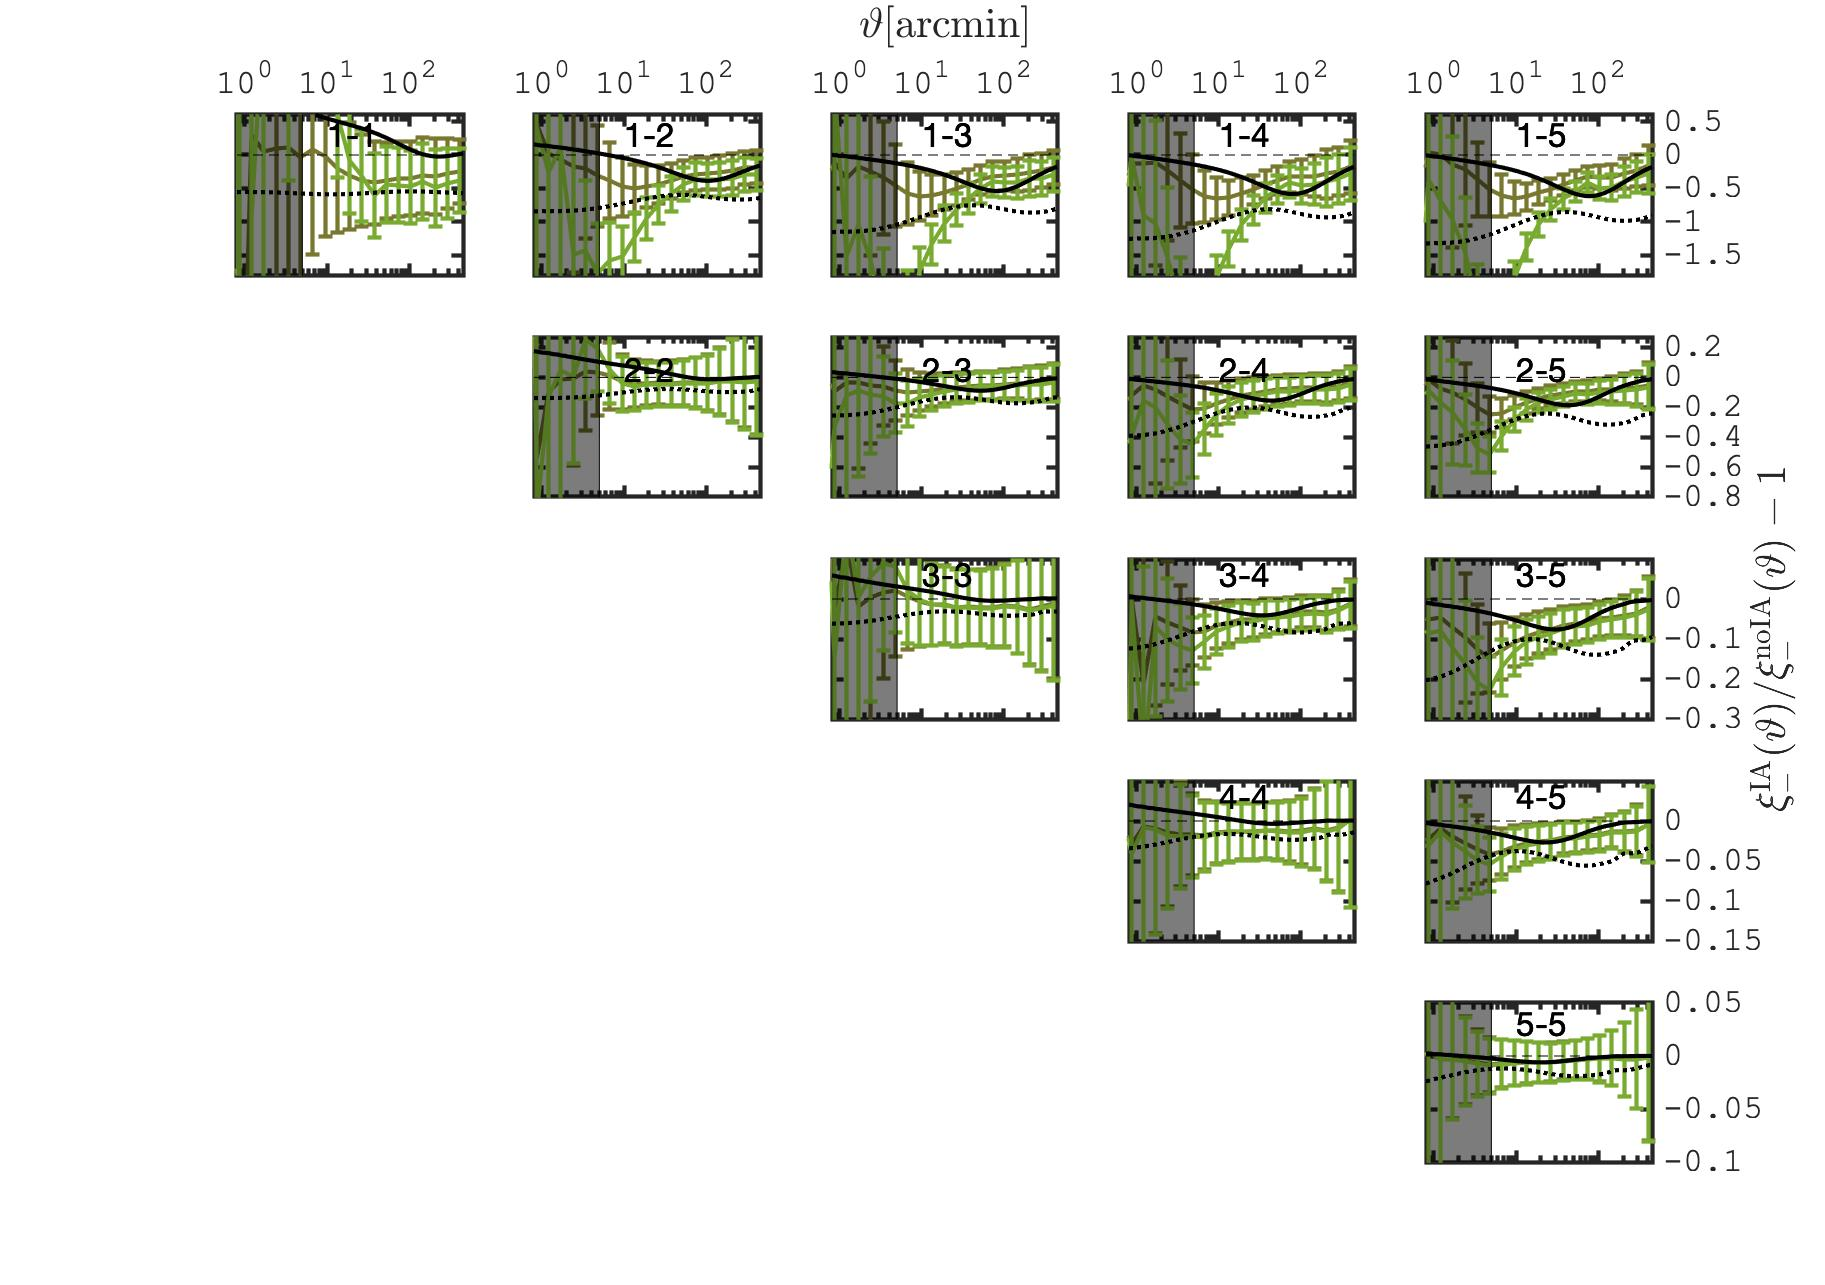
\includegraphics[width=\columnwidth]{graphs/frac_xim_IA1_skysim_TT_srd.jpg}
\caption{Same as Fig. \ref{fig:xi_NLA}, but for the TT model with $A_2=1.0$. Brown is smoothing scale of 0.5 arcmin, green is 0.1 arcmin. Here, the dashed black lines show the NLA predictions to better highlight the differences. }
\label{fig:xi_TT}
\end{figure*}

\begin{figure*}
%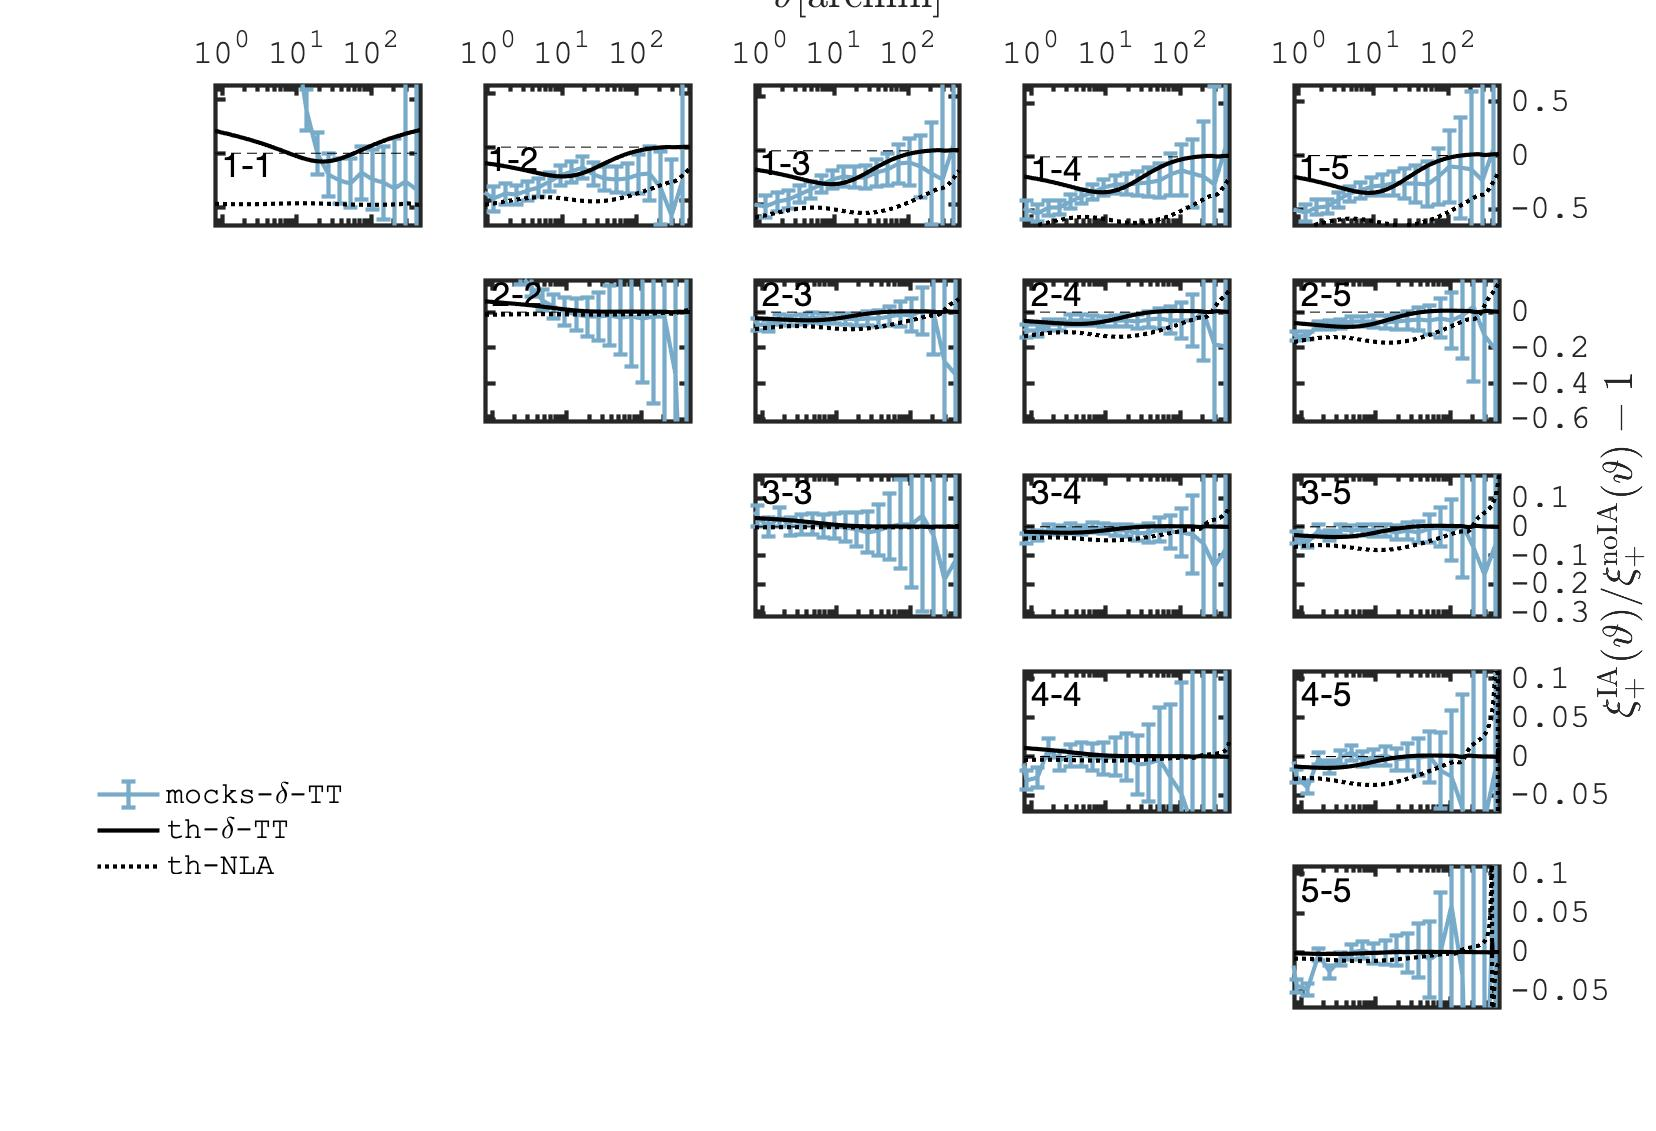
\includegraphics[width=\columnwidth]{graphs/frac_xip_C2_m1_skysim_deltaTT}
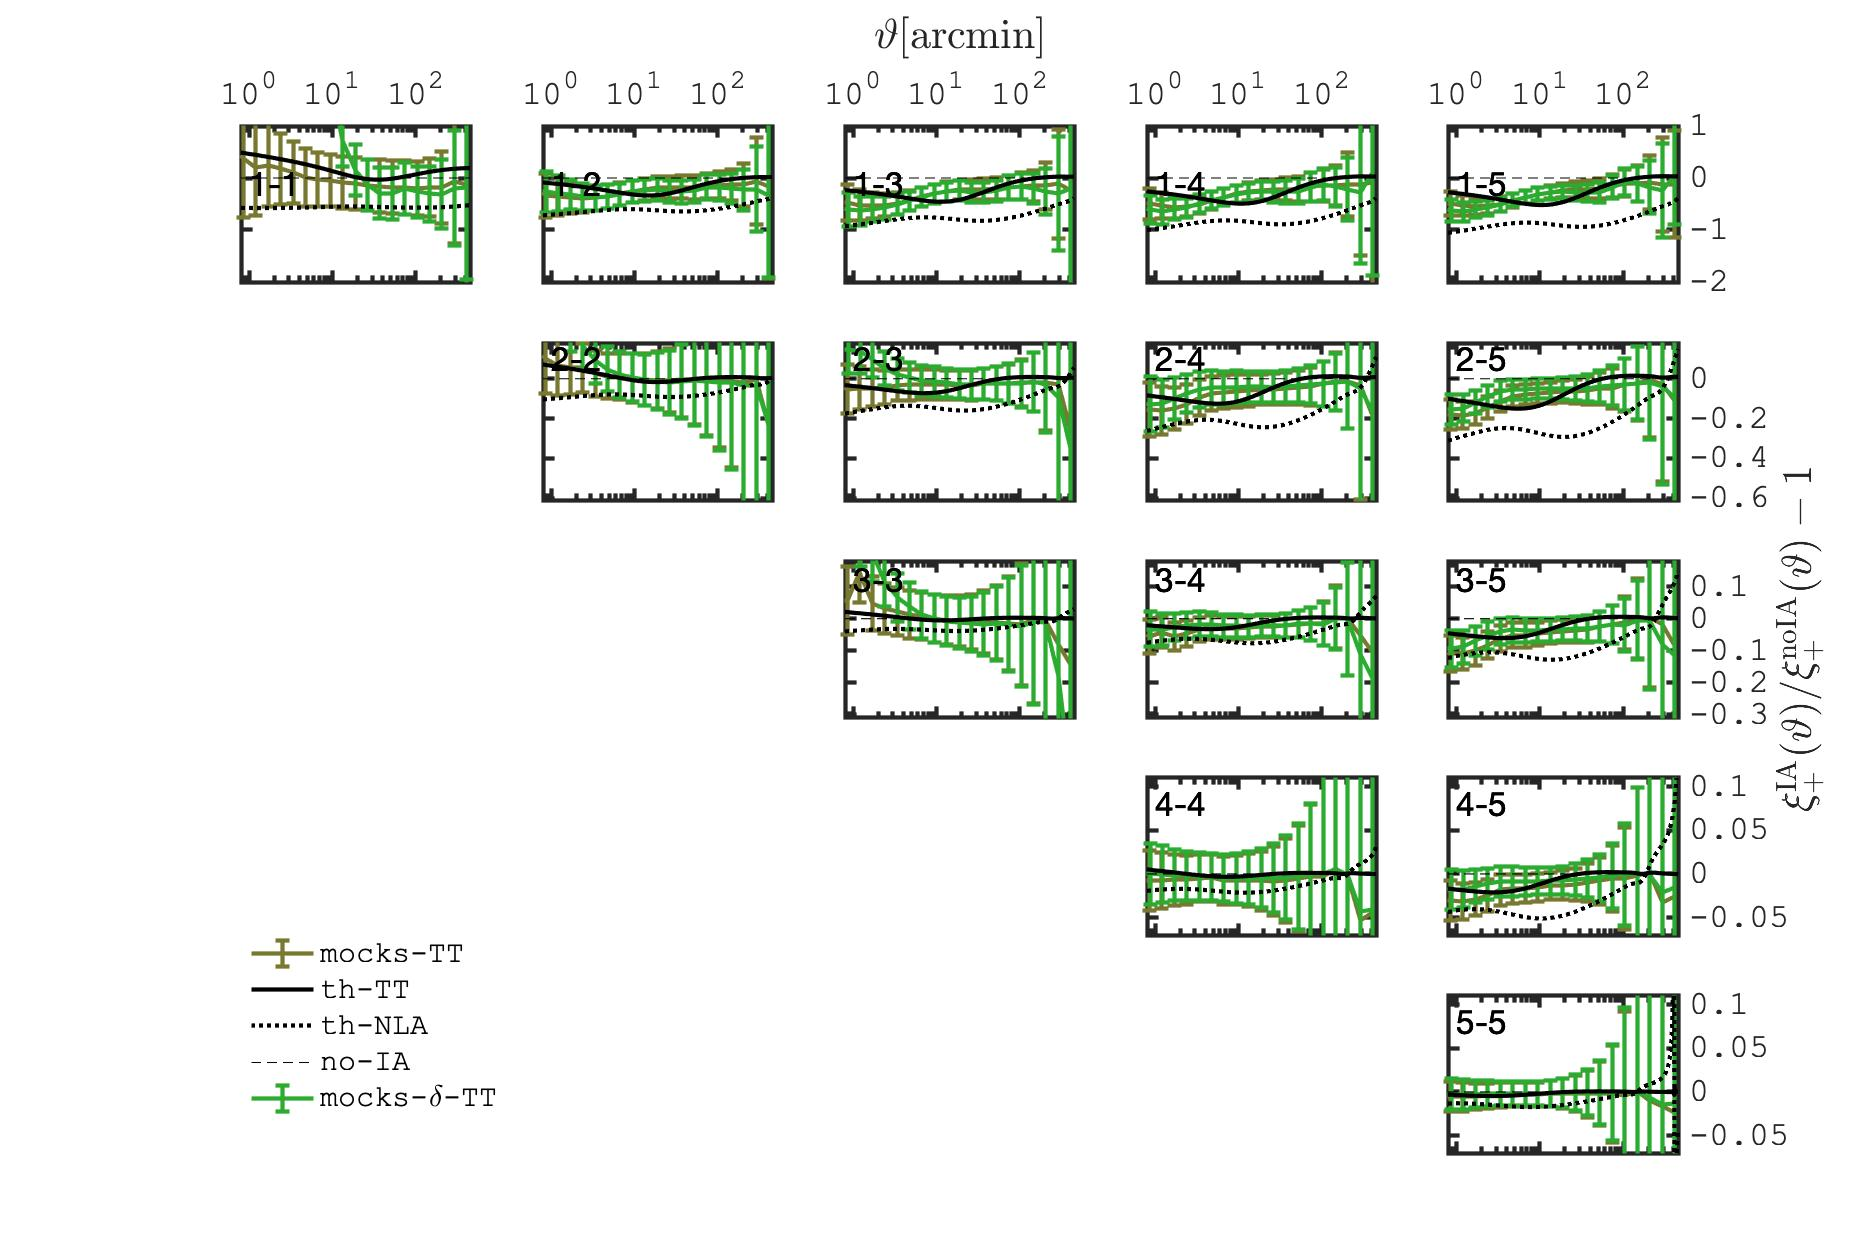
\includegraphics[width=\columnwidth]{graphs/frac_xip_IA1_skysim_deltaTT_srd.jpg}
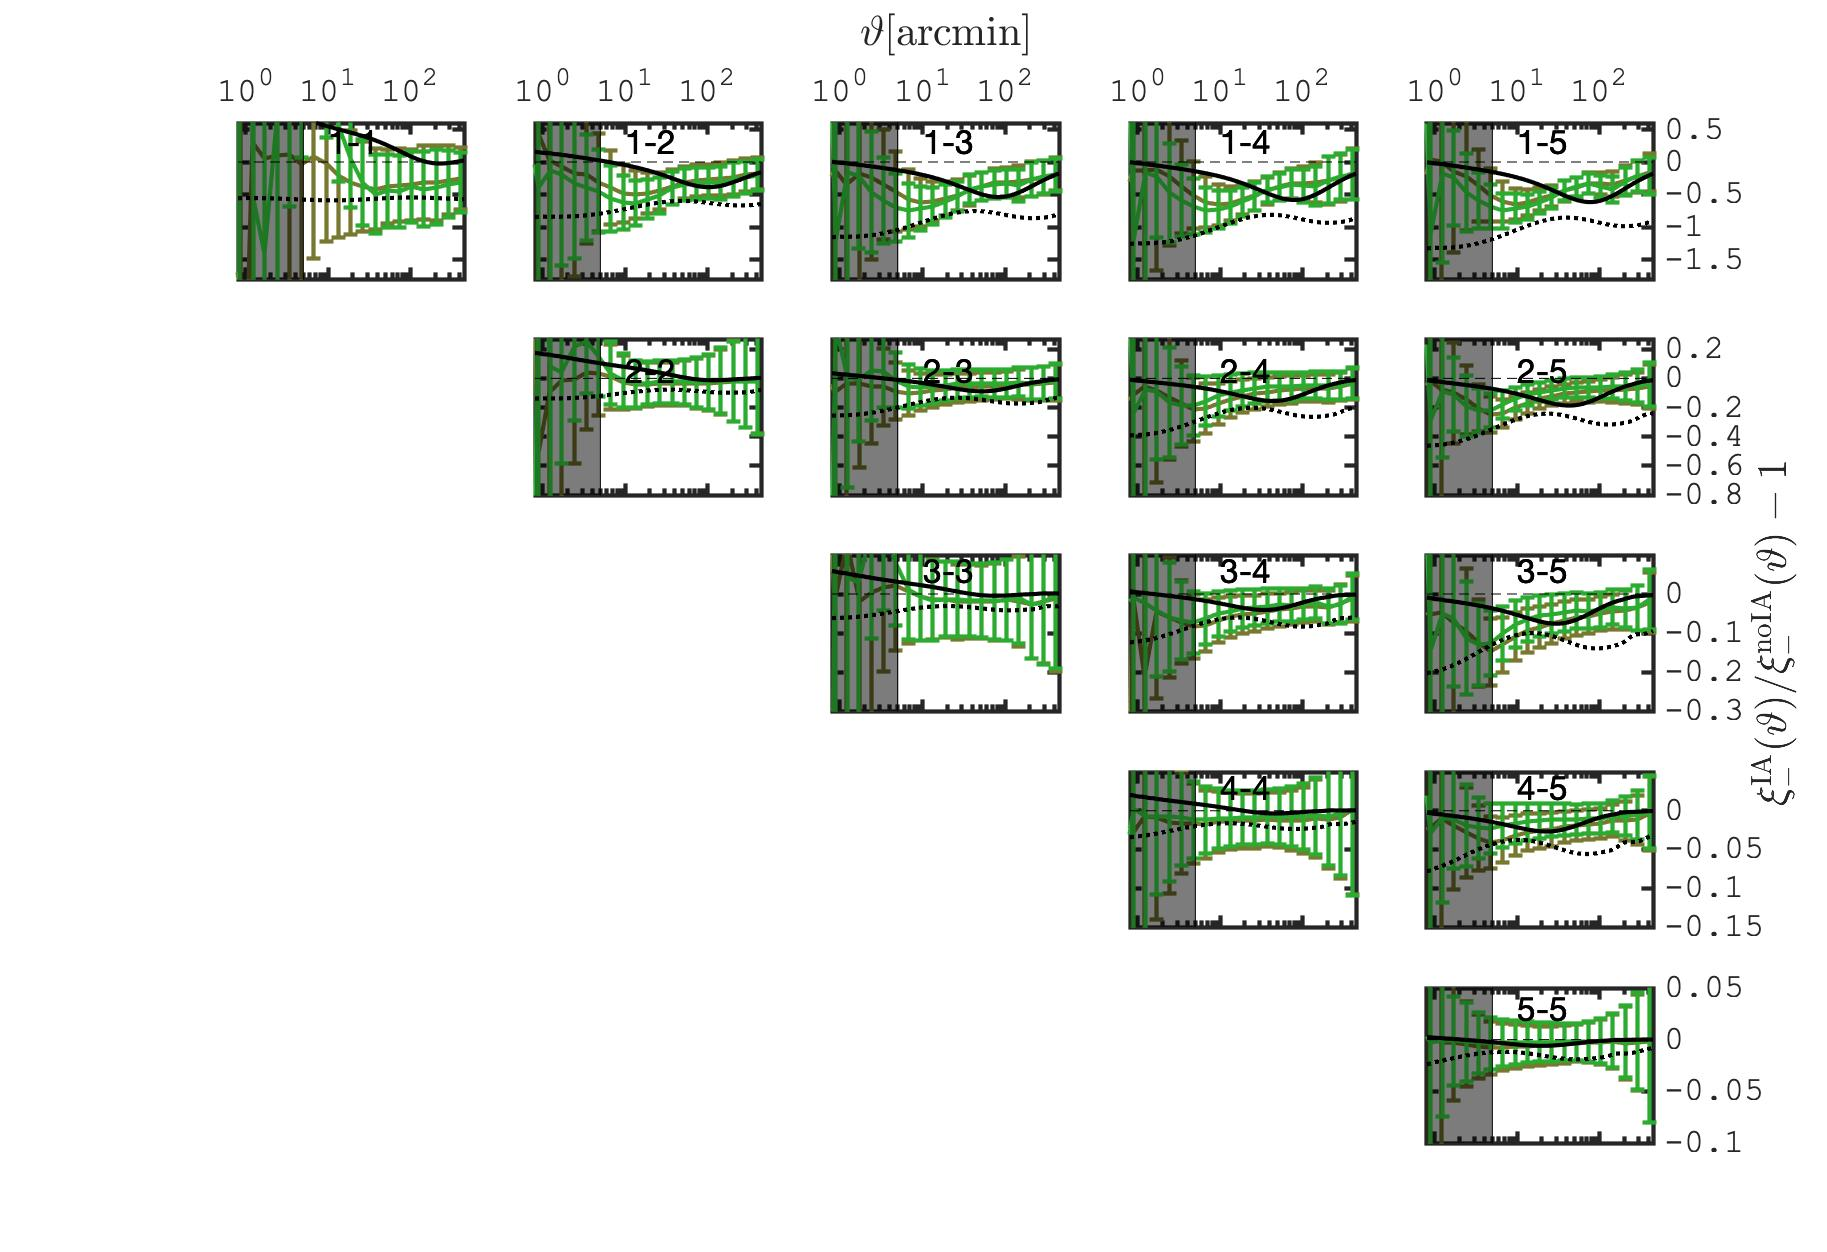
\includegraphics[width=\columnwidth]{graphs/frac_xim_IA1_skysim_deltaTT_srd.jpg}
\caption{Same as Fig. \ref{fig:xi_deltaNLA}, but comparing the TT (brown) and the $\delta$-TT  (green) models, with $A_2=1.0$, $b_{\rm TA}$ = 1.0, and only for smoothing of 0.5$h^{-1}$Mpc. }
\label{fig:xi_deltaTT}
\end{figure*}



%------------------------------
\subsubsection*{Extended-TT model}
\label{subsec:TT}

The extended-TT model, constructed by using the TT coupling on galaxies linearly tracing the underlying matter density, also needs to be calibrated. This has some degree of arbitrariness due to the absence of theoretical model to match it against. We choose to match the TT theory on large angular separation at all redshifts, physically motivated from the fact that this modified galaxy bias should not impact strongly scales that are much larger than galaxy clusters.
This therefore required us to lower the original ellipticities, especially at low $z$: $\epsilon^{{\rm IA}, \delta{\rm TT}}(z<0.5) \rightarrow \epsilon^{{\rm IA}, \delta{\rm TT}} /2.5$ as for the normal TT model, further followed by a global $\epsilon^{{\rm IA}, \delta{\rm TT}} \rightarrow \epsilon^{{\rm IA}, \delta{\rm TT}}/20.0$ rescaling. This is a large calibration condition, which compensate for the overly strong coupling computed from our simulations. The results are shown in Fig. \ref{fig:xi_deltaTT}, where we observed that the deviations with respect to the TT model occur at small angular scales ($\vartheta < $ 20 arcmin) in $\xi_+$, and for the lowest redshifts. Although this model is harder to match with current theoretical IA model, it provides a good example with which we can study the impact of IA mis-modelling, e.g. analysing this model with the TATT predictions, similar to the investigations of \citet{Paopiamsap2024}.


%------------------------------
\subsubsection*{HOD-TATT model}
\label{subsec:HOD}


%--------------
\begin{figure*}
%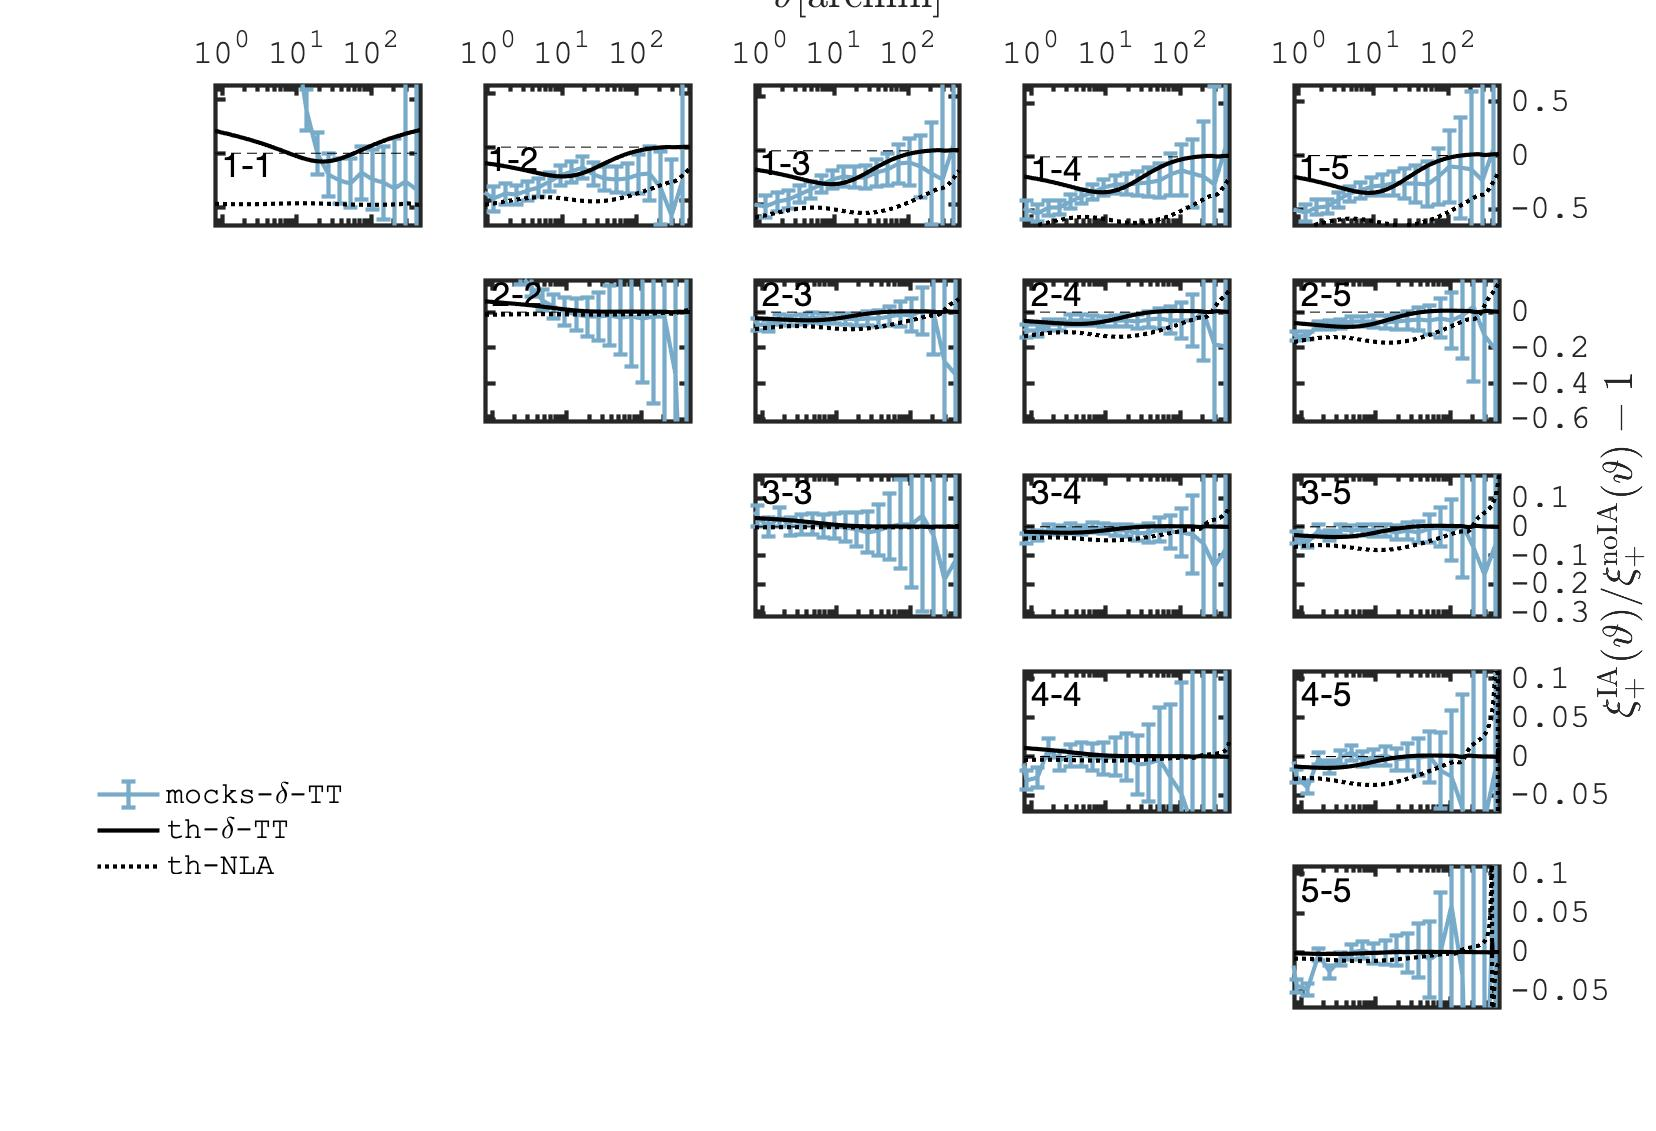
\includegraphics[width=\columnwidth]{graphs/frac_xip_C2_m1_skysim_deltaTT}
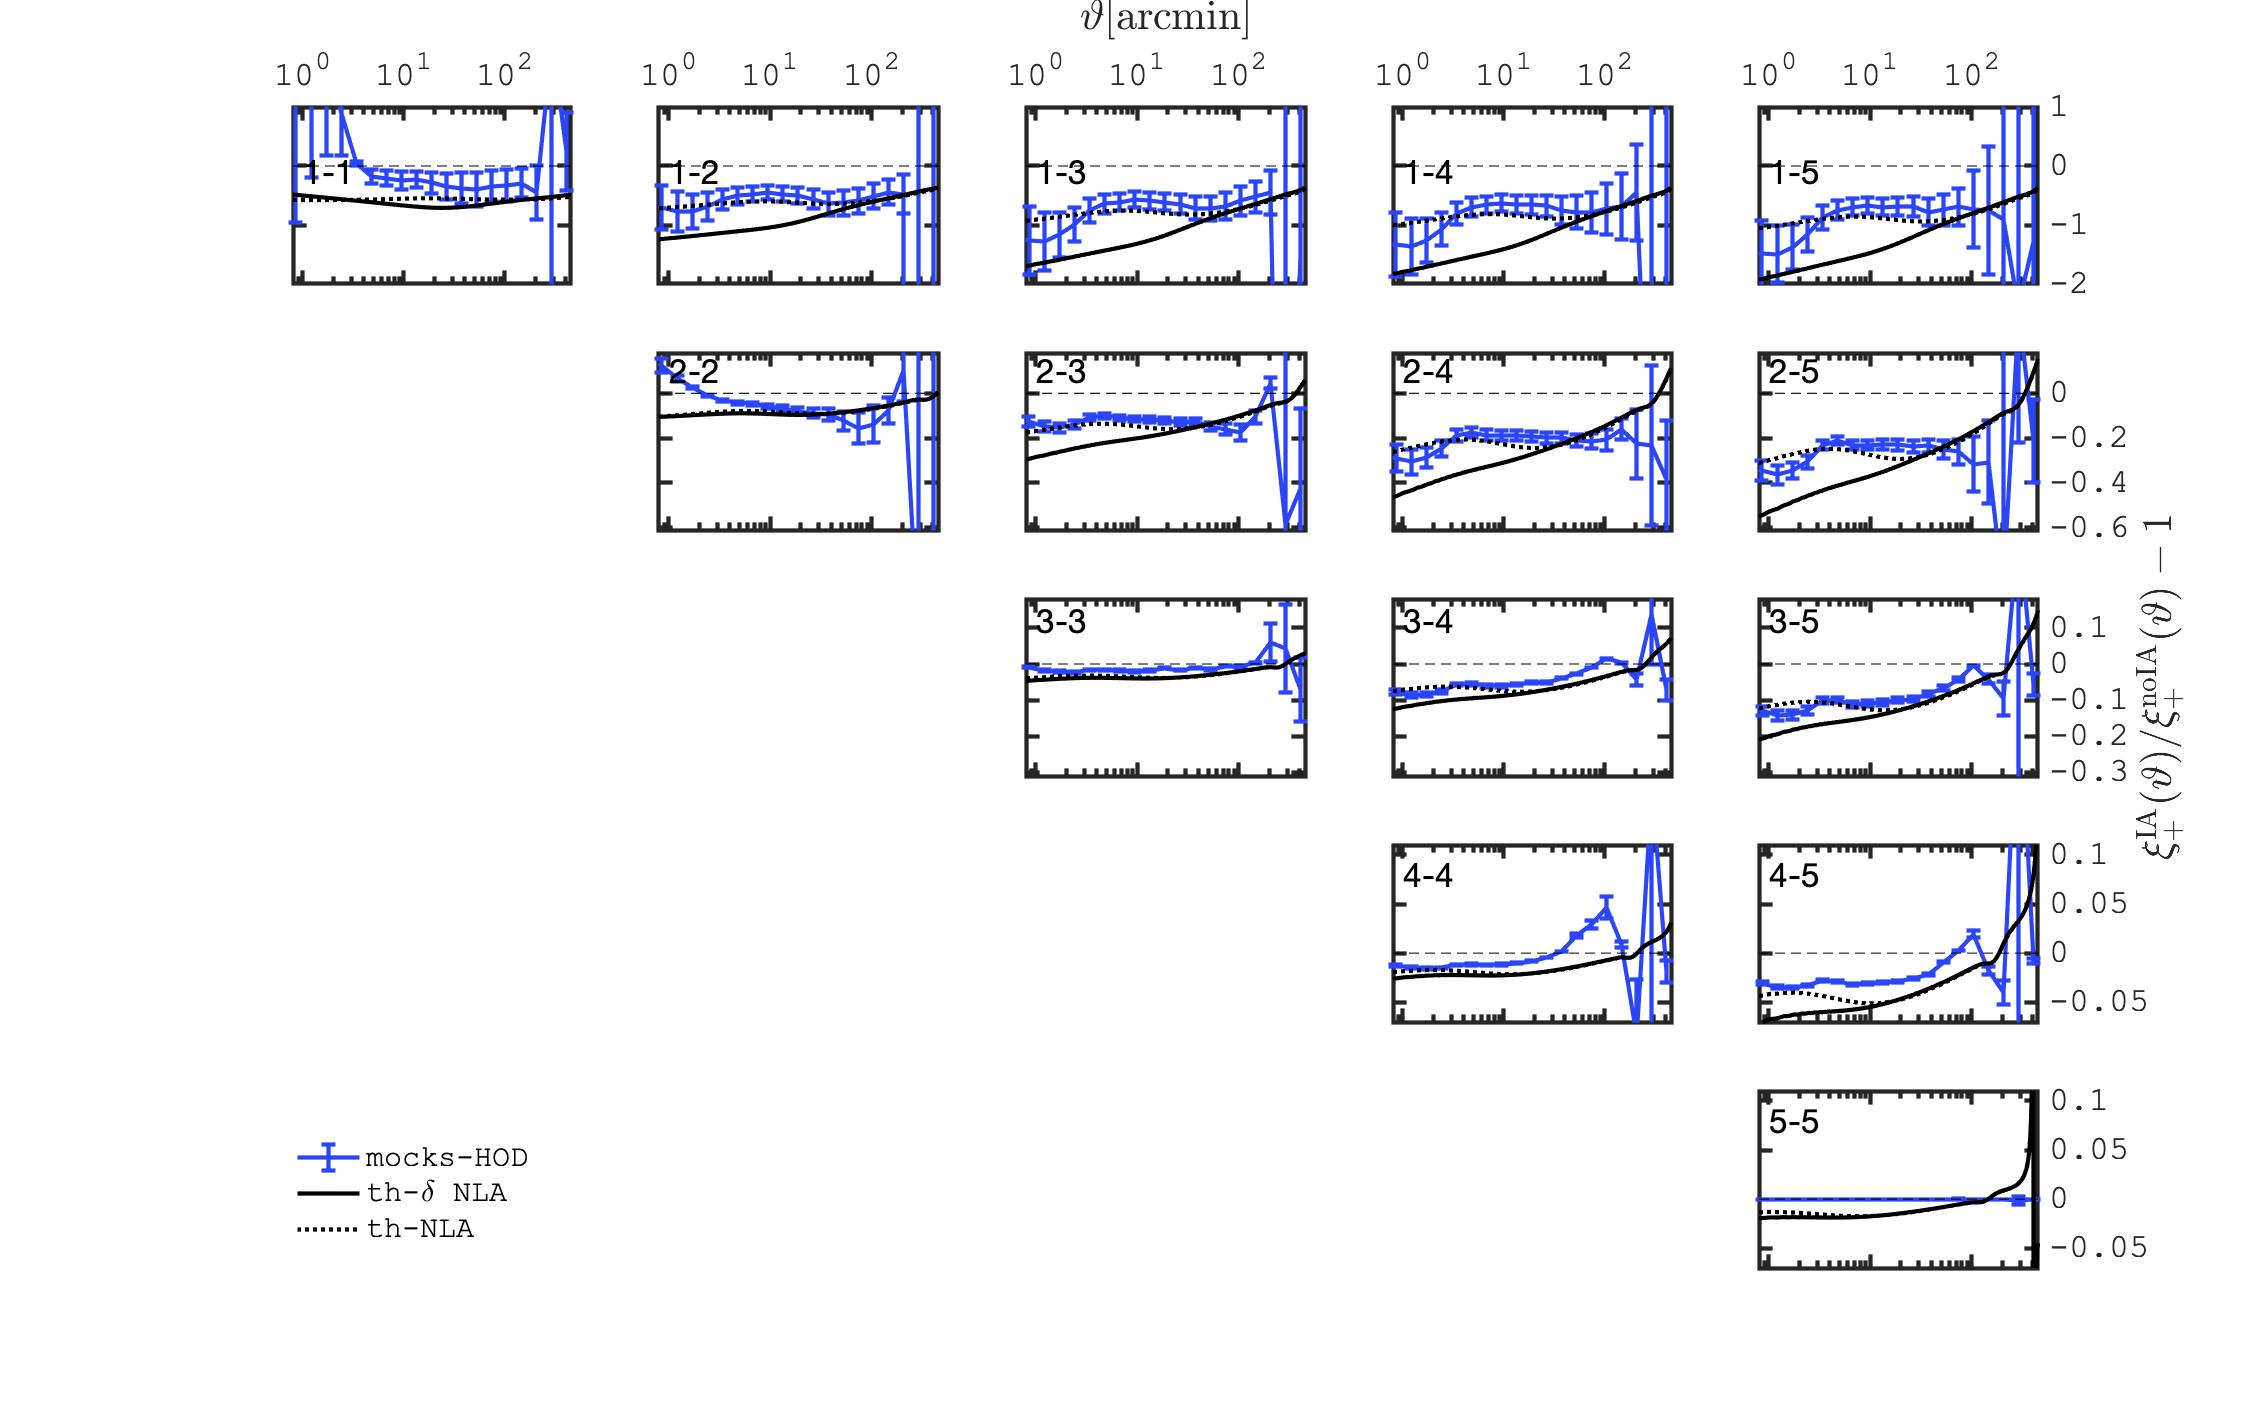
\includegraphics[width=\columnwidth]{graphs/frac_xip_sims_HOD.jpg}
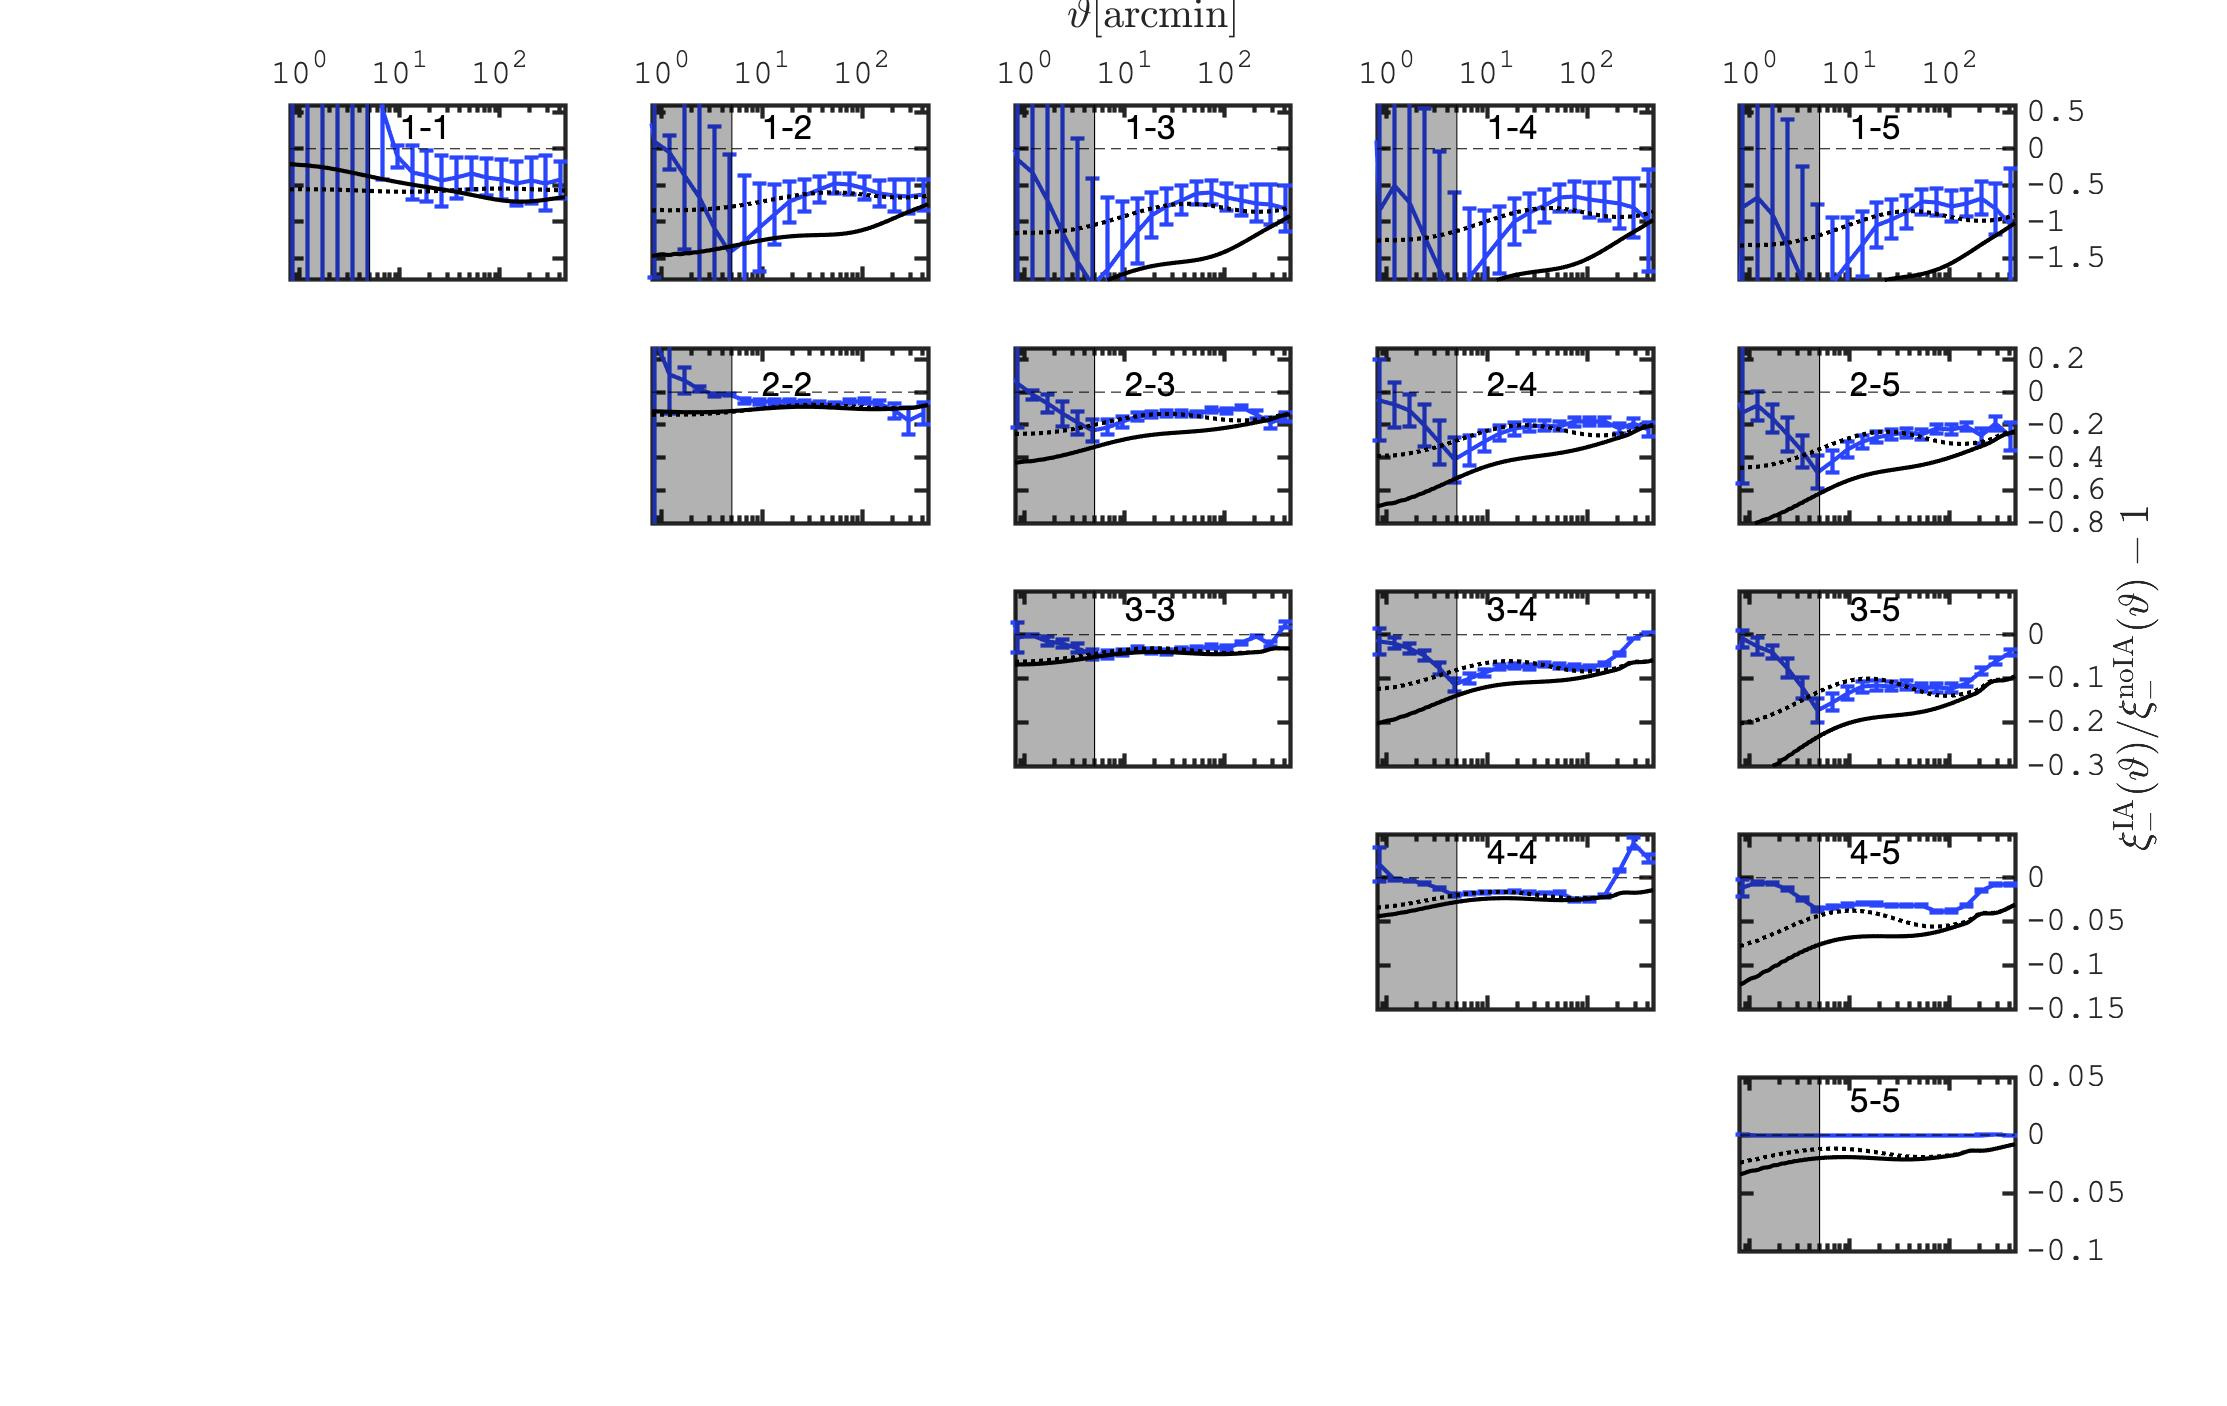
\includegraphics[width=\columnwidth]{graphs/frac_xim_sims_HOD.jpg}
\caption{Same as Fig. \ref{fig:xi_deltaNLA}, but showing the HOD galaxies with shapes linearly coupled with the tidal field. }
\label{fig:xi_hod_nla}
\end{figure*}

%--------------
\begin{figure*}
%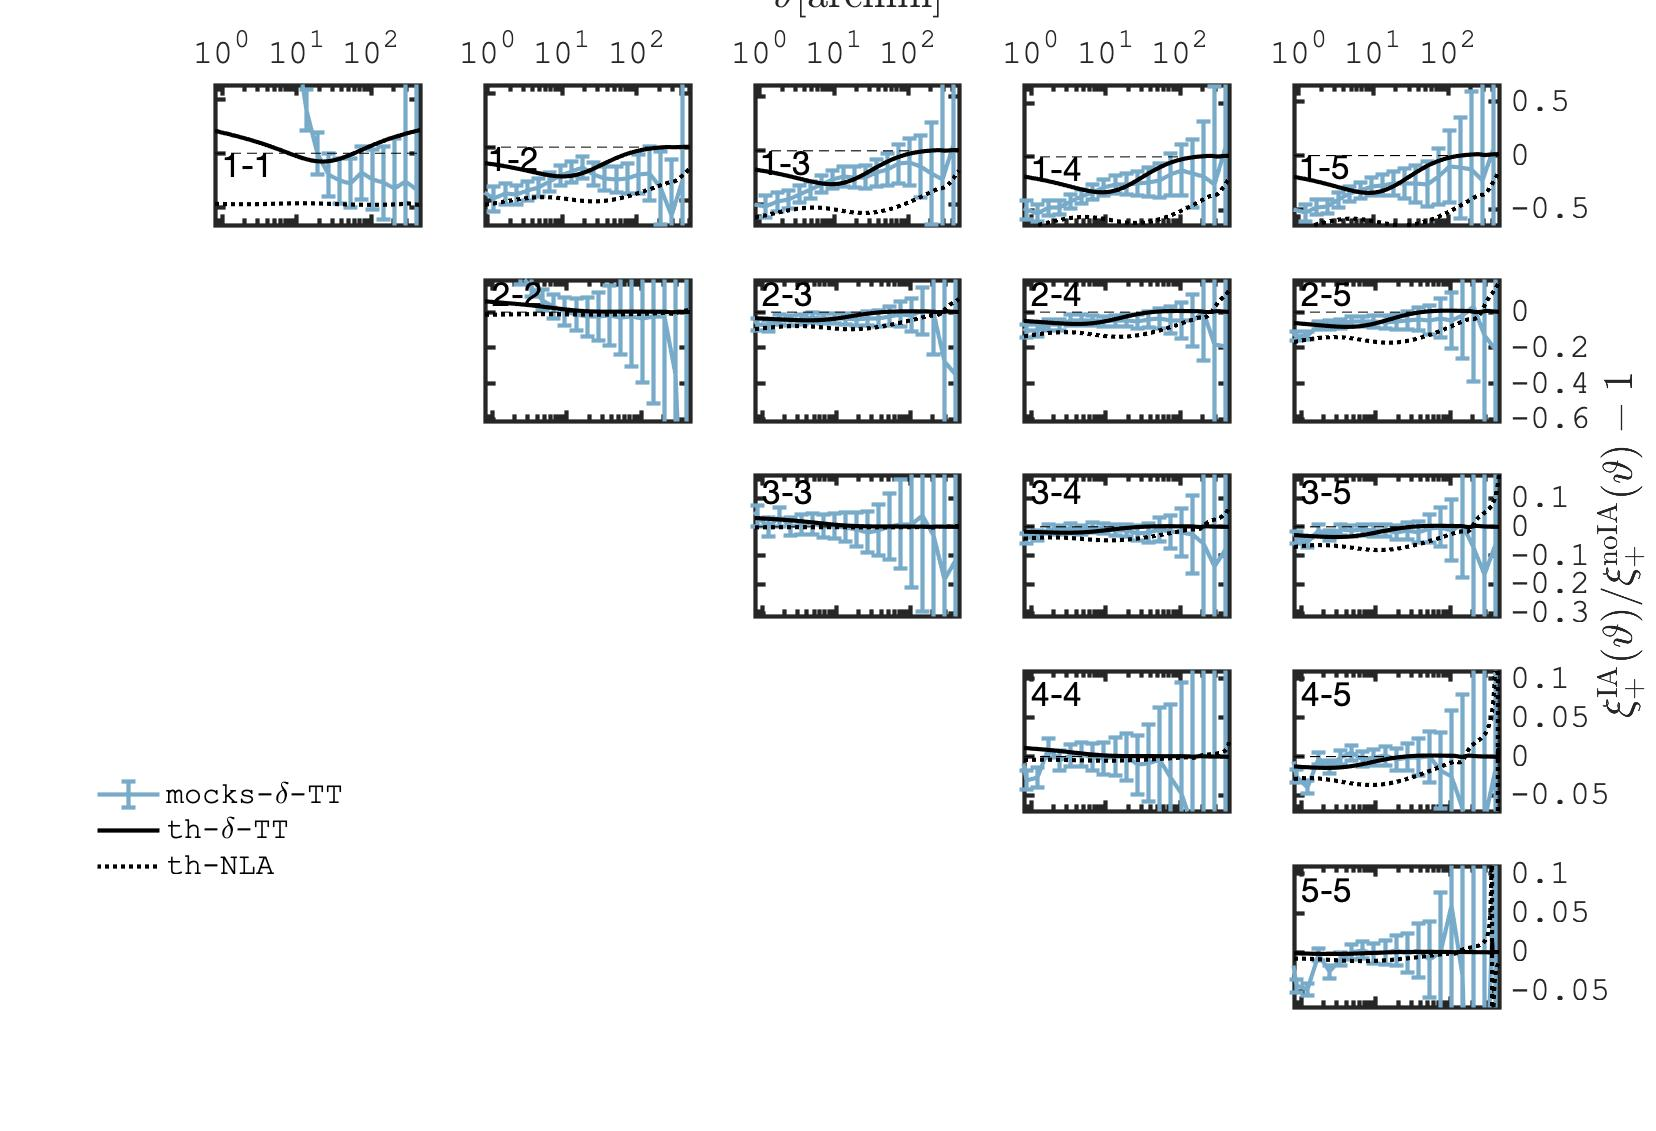
\includegraphics[width=\columnwidth]{graphs/frac_xip_C2_m1_skysim_deltaTT}
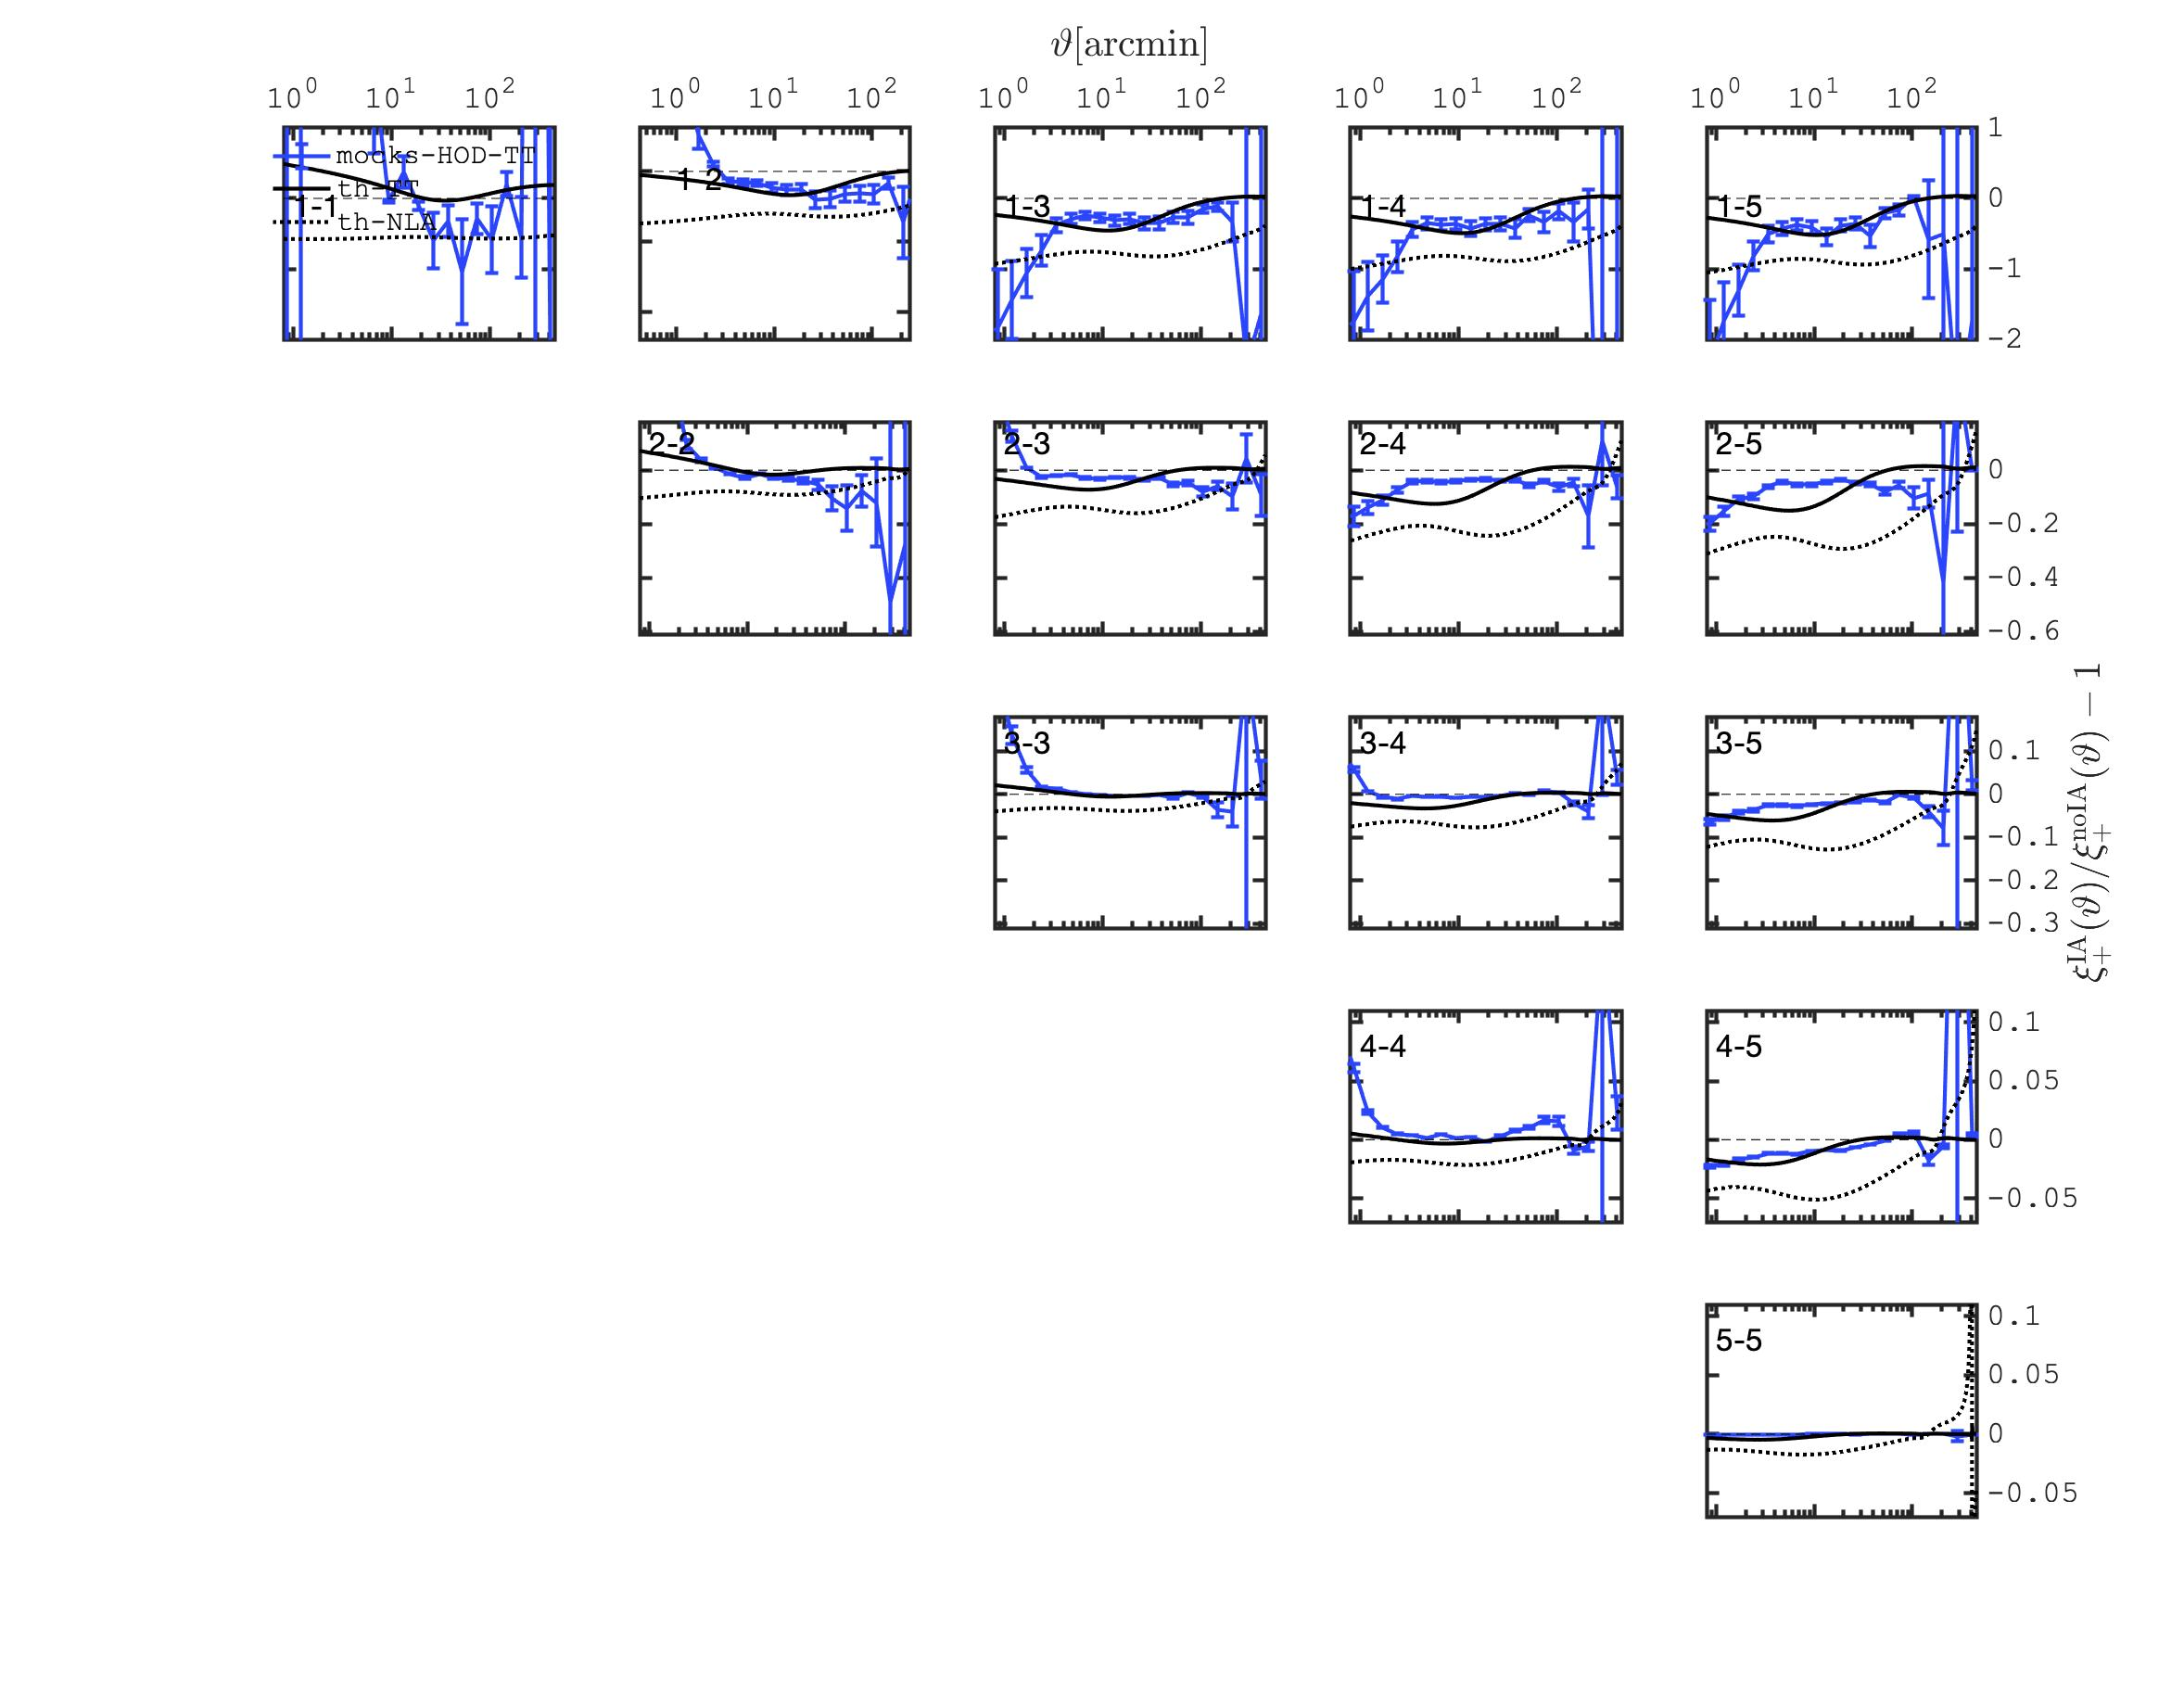
\includegraphics[width=\columnwidth]{graphs/frac_xip_sims_HOD_TT.jpg}
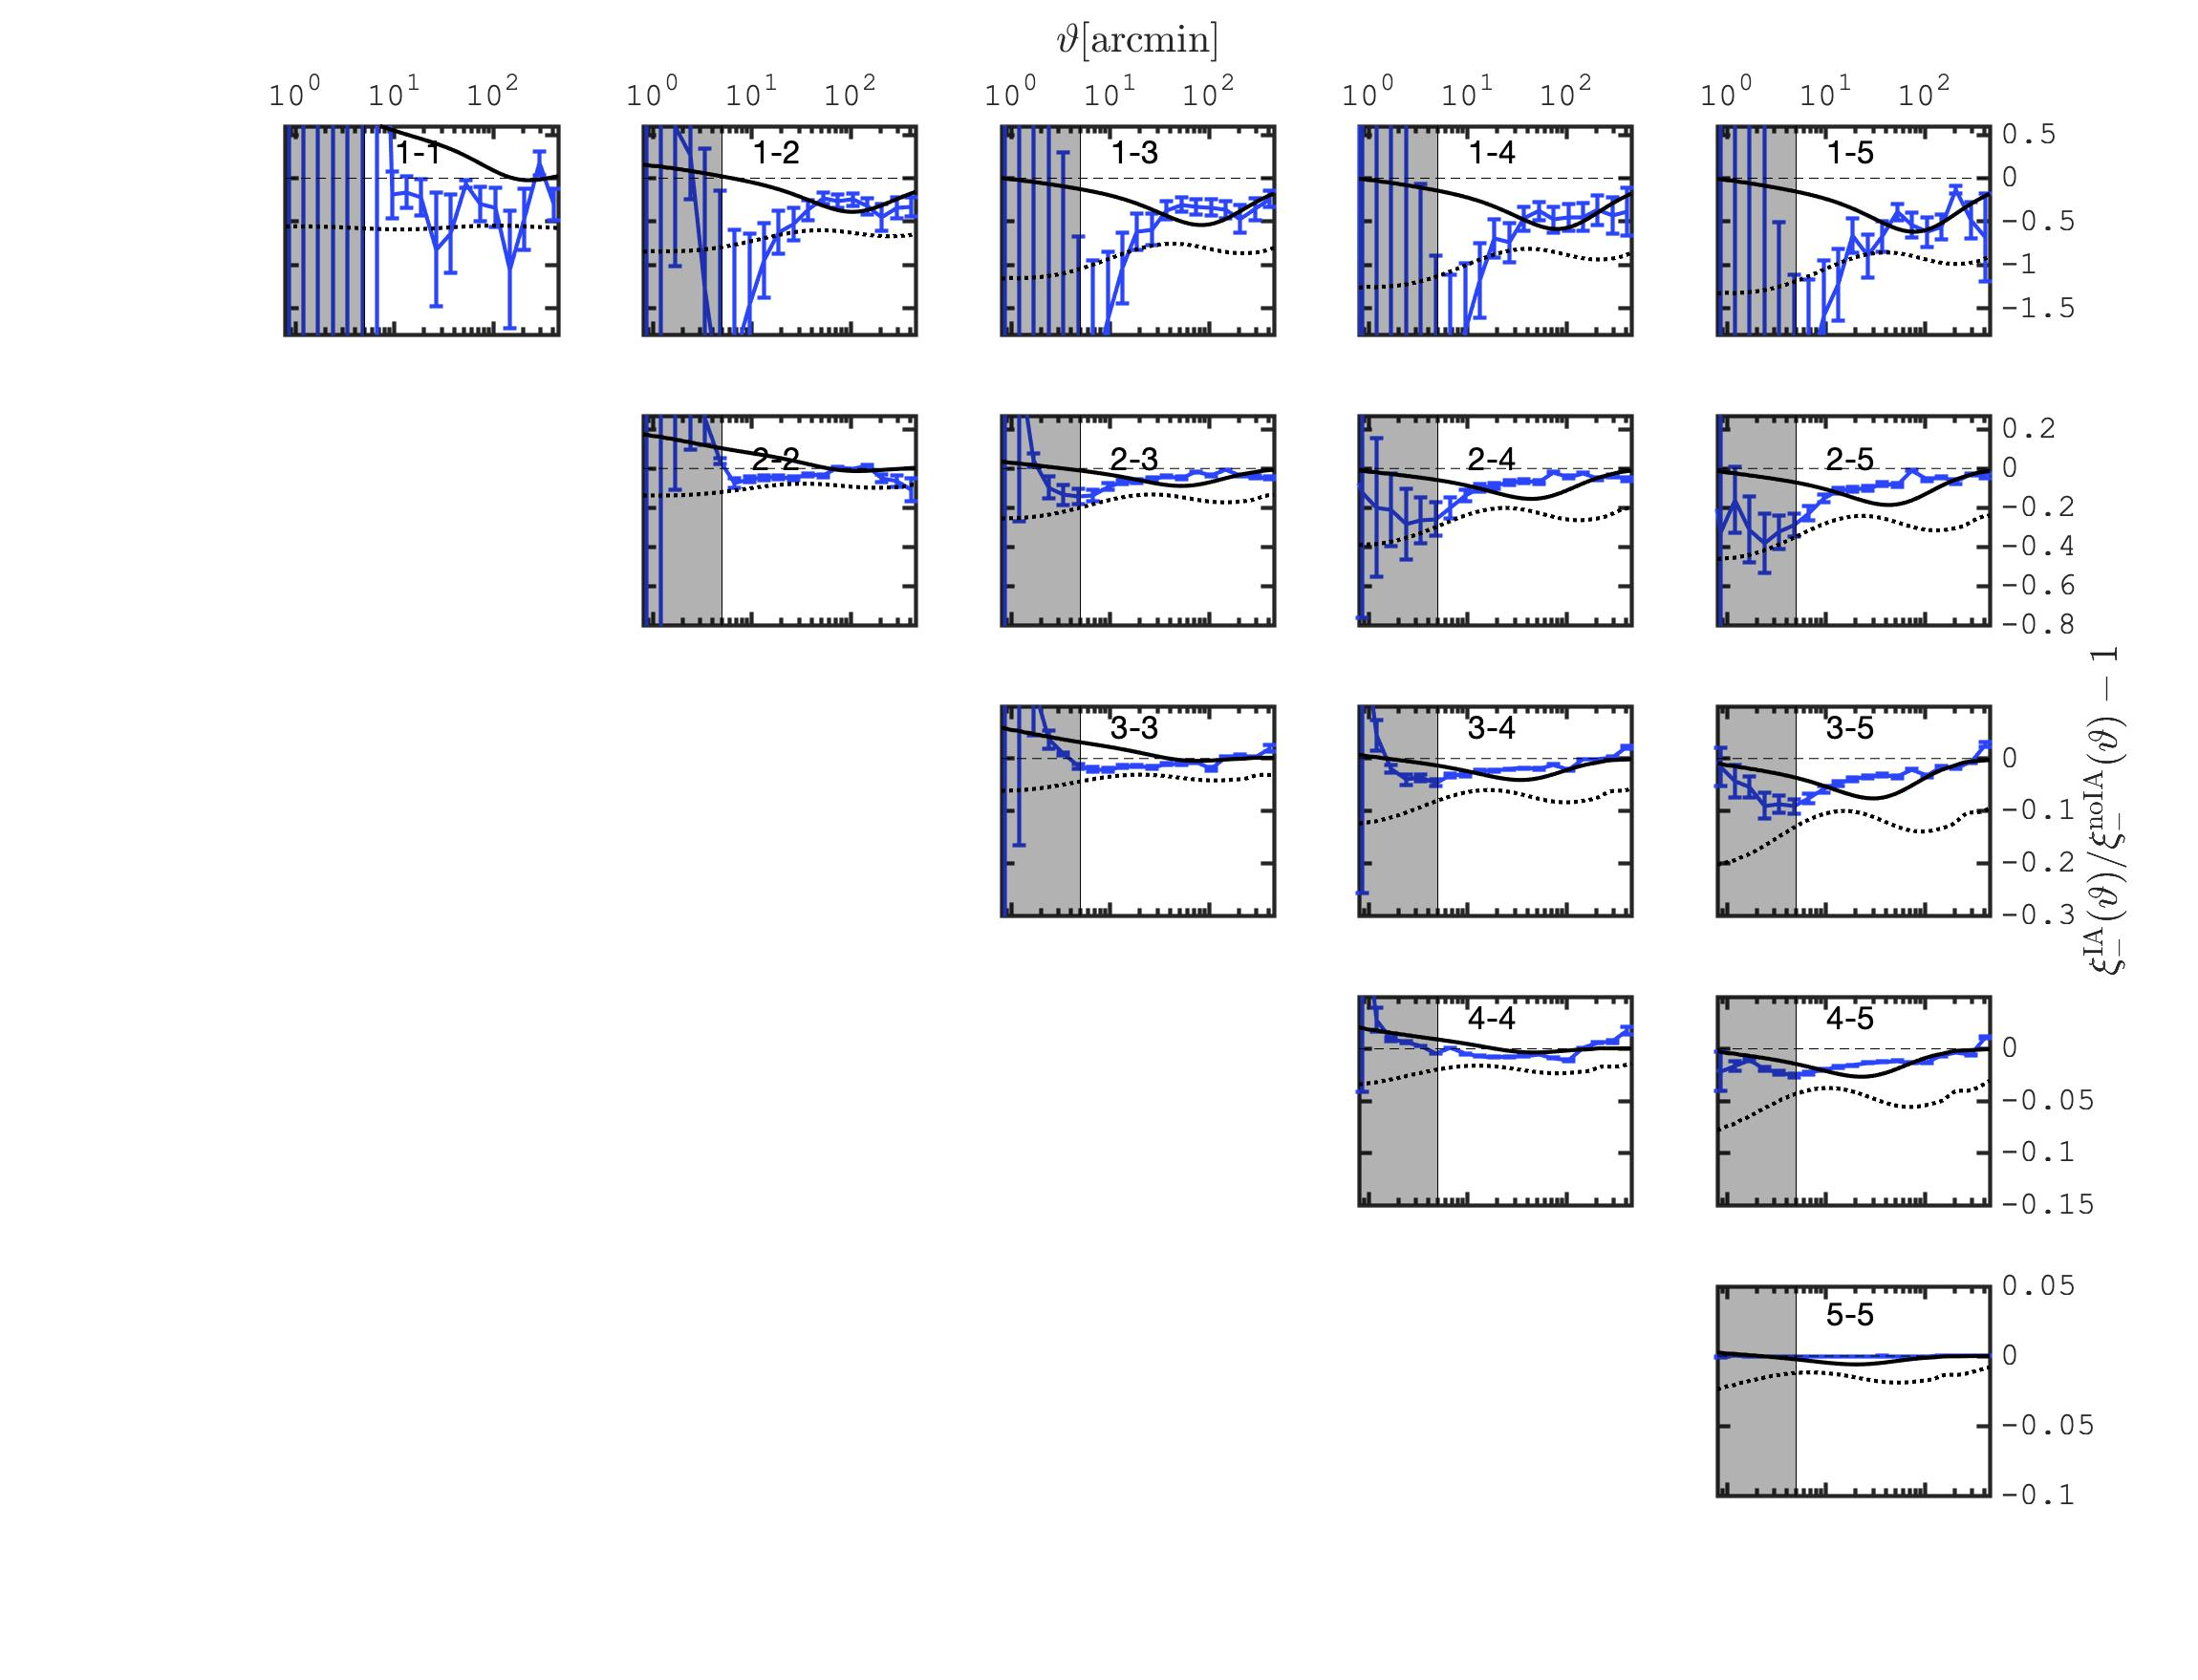
\includegraphics[width=\columnwidth]{graphs/frac_xim_sims_HOD_TT.jpg}
\caption{Same as Fig. \ref{fig:xi_deltaTT}, but showing the HOD galaxies with shapes quadratically coupled with the tidal field. }
\label{fig:xi_hod_tt}
\end{figure*}


%The NLA and extended-NLA models respectively assume a null and a linear bias between the source galaxies and the underlying matter field, both of which are approximations to the galaxy-dark matter connection.
%In fact, galaxies populate dark matter over-densities in a more complex manner \citep{GalaxyPopulationPapers}, which is better described by the Halo Occupation Distribution approach (HOD hereafter).
The largest difference between the previous models and those based on HOD galaxies is that the latter are non-linear biased tracers of the matter distribution, which means that a larger number can populate regions of large over-densities, where the tidal fields are generally stronger. We therefore expect the impact of IA to be stronger in this case. We show in Figs. \ref{fig:xi_hod_nla} and \ref{fig:xi_hod_tt} show the results from the HOD-NLA  and HOD-TT models, which together make up our HOD-TATT. One of the most interesting features is that the HOD-NLA closely follows the normal NLA predictions over a large range of scales, suggesting that the impact of the non-linear galaxy bias is sub-dominant down to a few acrmin. We also observe a small-angle up-turn in bins 1-1 and 2-2, which can be attributed to mismodelling the $II$ term (as it is the case for the extended-NLA, see the discussion above) {\it (Also what's goiing on with bin 5? There seems to be no IA signal there...)}. 



\subsection{Validation with full inference}
 \label{sec:inference}

 
 \begin{table}
   \centering
   \caption{Priors used in the likelihood sampling. {\it (verify these numbers with Niko)}}
   \tabcolsep=0.11cm
      \begin{tabular}{@{} cccccccc @{}} % Column formatting, @{} suppresses leading/trailing space
      \hline
      \hline
       Parameter       &  range & prior \\
       \hline
       Cosmology\\ 
       $\Omega_{\rm m}$ &[0.1, 0.55] & Flat\\
       $S_8$ & [0.6, 0.9] & Flat\\
       \hline
       IA\\
       $A_{\rm IA}$ & [-5, 5]&  Flat\\                    
        $b_{\rm TA}$ & [0, 2] & Flat\\
        $C_2$ & [-5, 5] & Flat\\
     \hline
    \hline 
    \end{tabular}
    \label{table:priors}
\end{table}

 

\begin{figure}
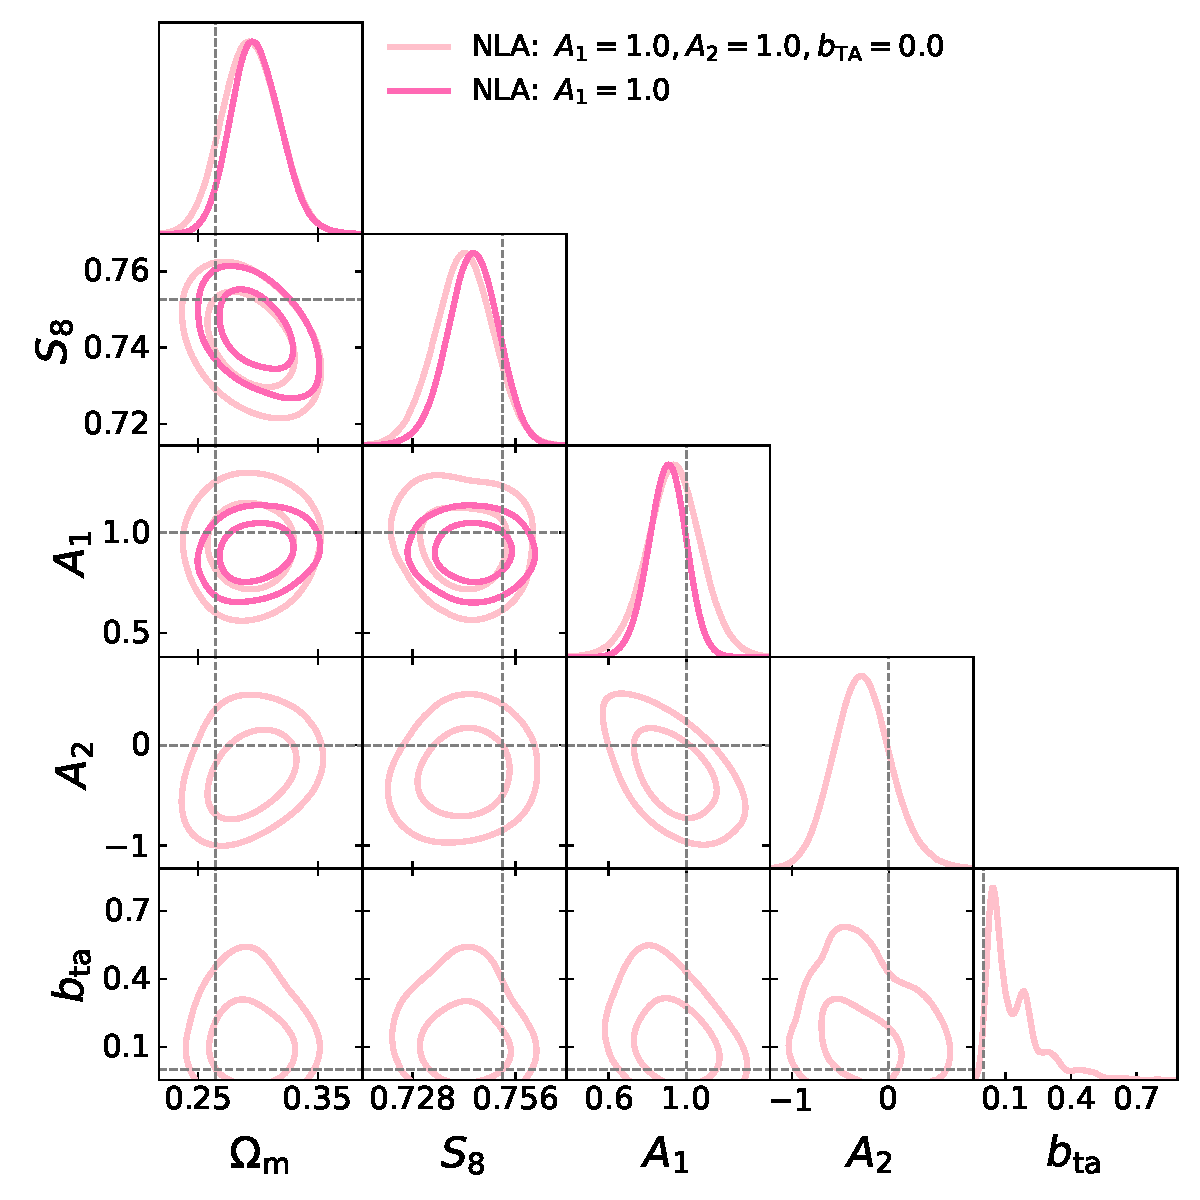
\includegraphics[width=\columnwidth]{graphs/NLA_1_0_0.pdf}
\caption{Cosmological inference from the NLA-infused simulations, with all 3 IA parameters varied (light pink) and with varying A1 only (dark pink).
The cross-hairs represent the truth as fixed in the {\it Outer Rim} $N$-body simulations \citep{OuterRim}.}
\label{fig:corner_nla_all_ia_params}
\end{figure}
\begin{figure}
%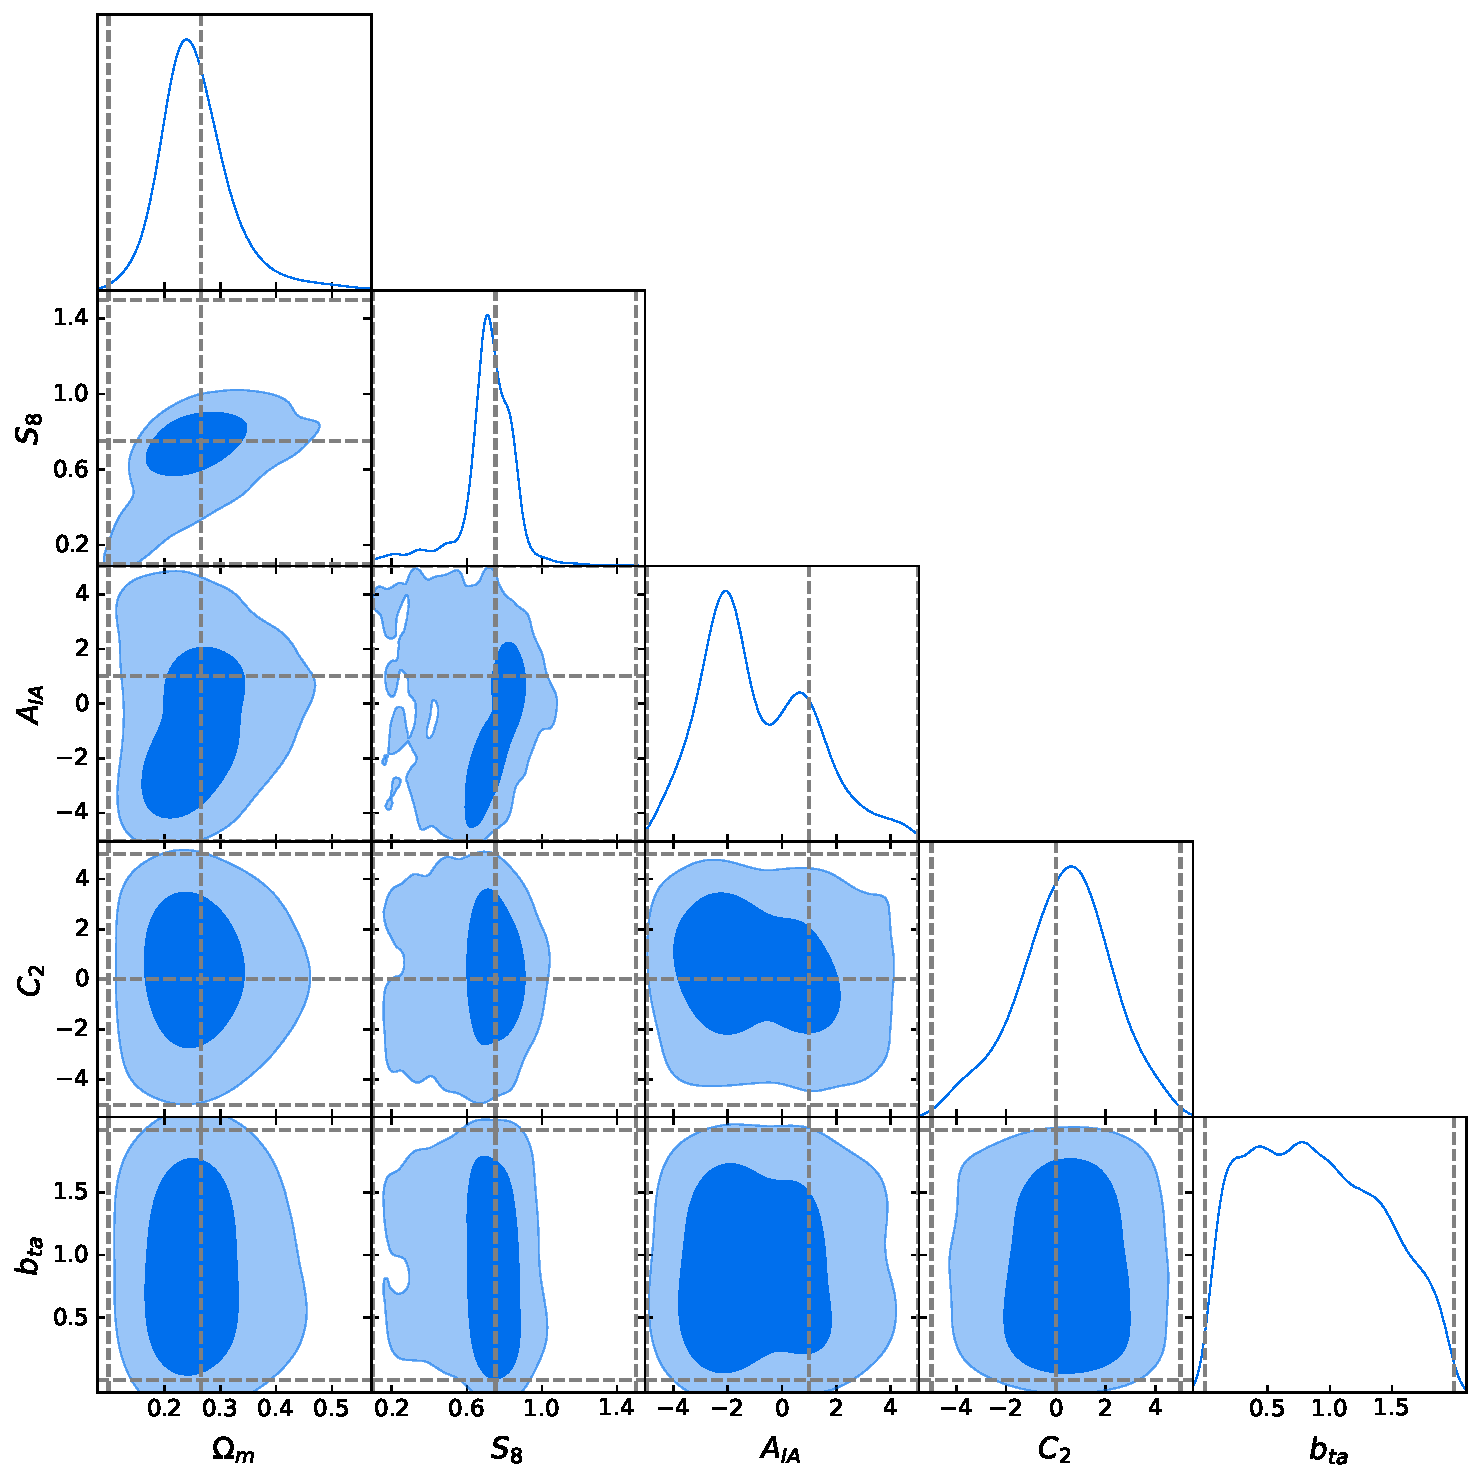
\includegraphics[width=\columnwidth]{graphs/triangle_nla_5D.pdf}
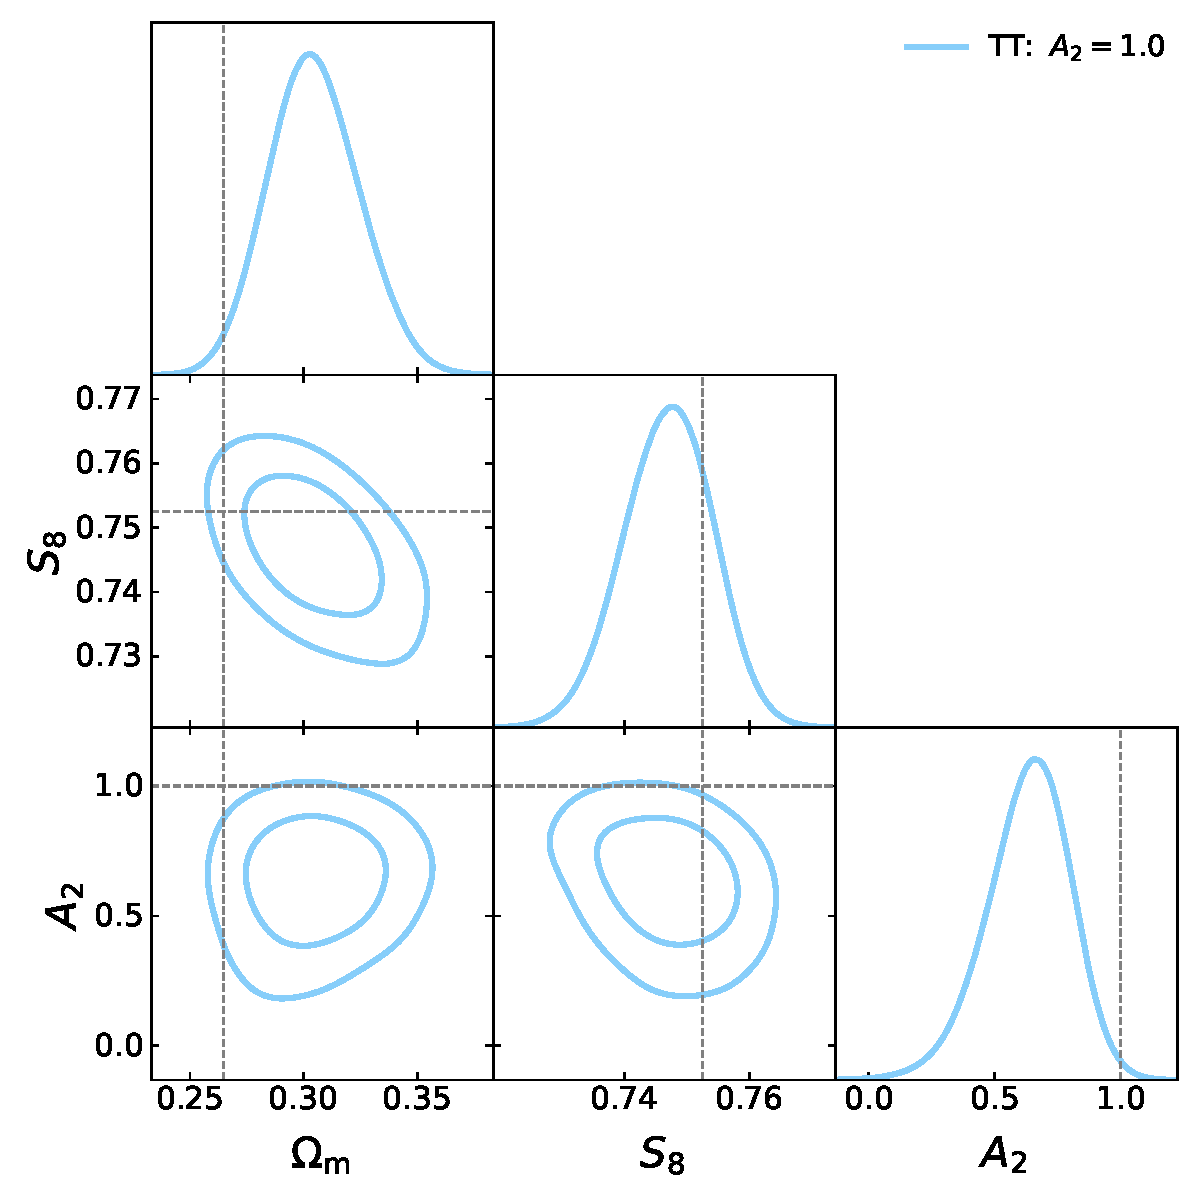
\includegraphics[width=\columnwidth]{graphs/TT_a2.pdf}
\caption{Cosmological inference from the TT-infused simulations, with $A_2$ varied ($A_1$ and $b_\mathrm{TA}$ fixed). The cross-hairs represent the truth as fixed in the {\it Outer Rim} $N$-body simulations \citep{OuterRim}.}
\label{fig:triangle_tt_vary_a2}
\end{figure}
\begin{figure}
%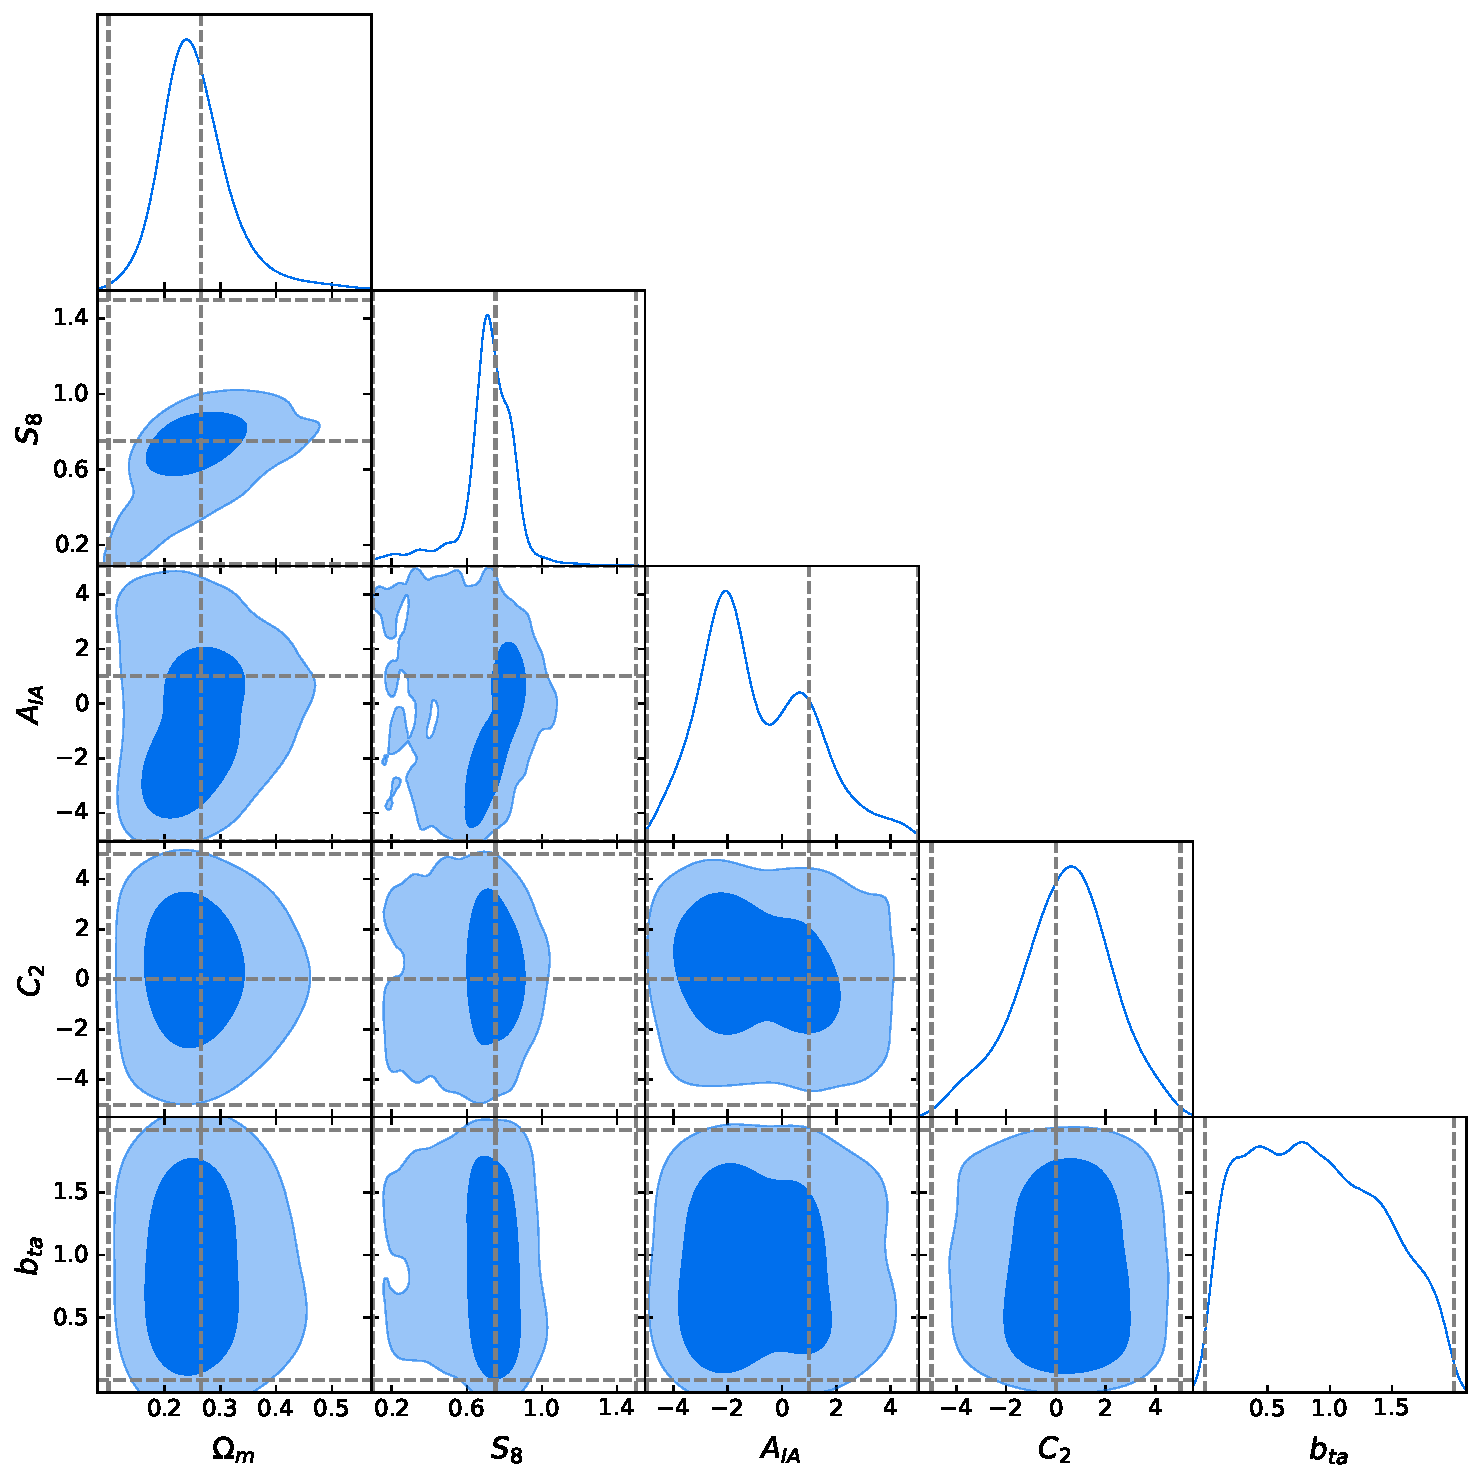
\includegraphics[width=\columnwidth]{graphs/triangle_nla_5D.pdf}
%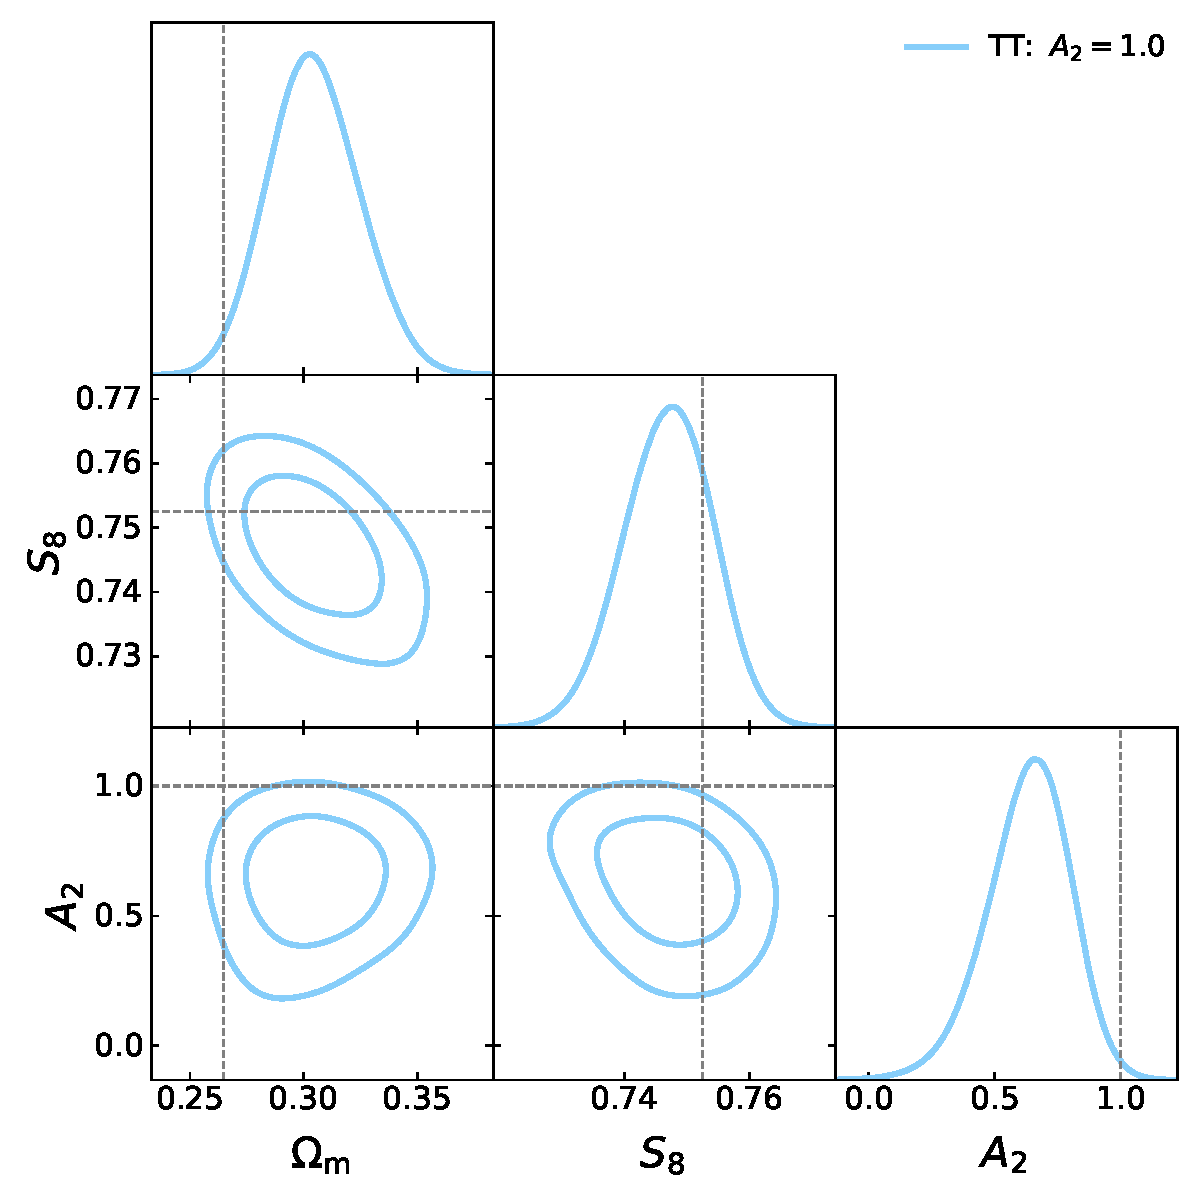
\includegraphics[width=\columnwidth]{graphs/TT_a2.pdf}
\includegraphics[width=\columnwidth]{graphs/delta_NLA.pdf}
\caption{Cosmological inference from the extended NLA-infused simulations, where either all three TATT parameters are varied.  {\it(fix axis labels and legend, remove one of the curves.)}}
\label{fig:triangle_deltaNLA_combo}
\end{figure}
\begin{figure}
%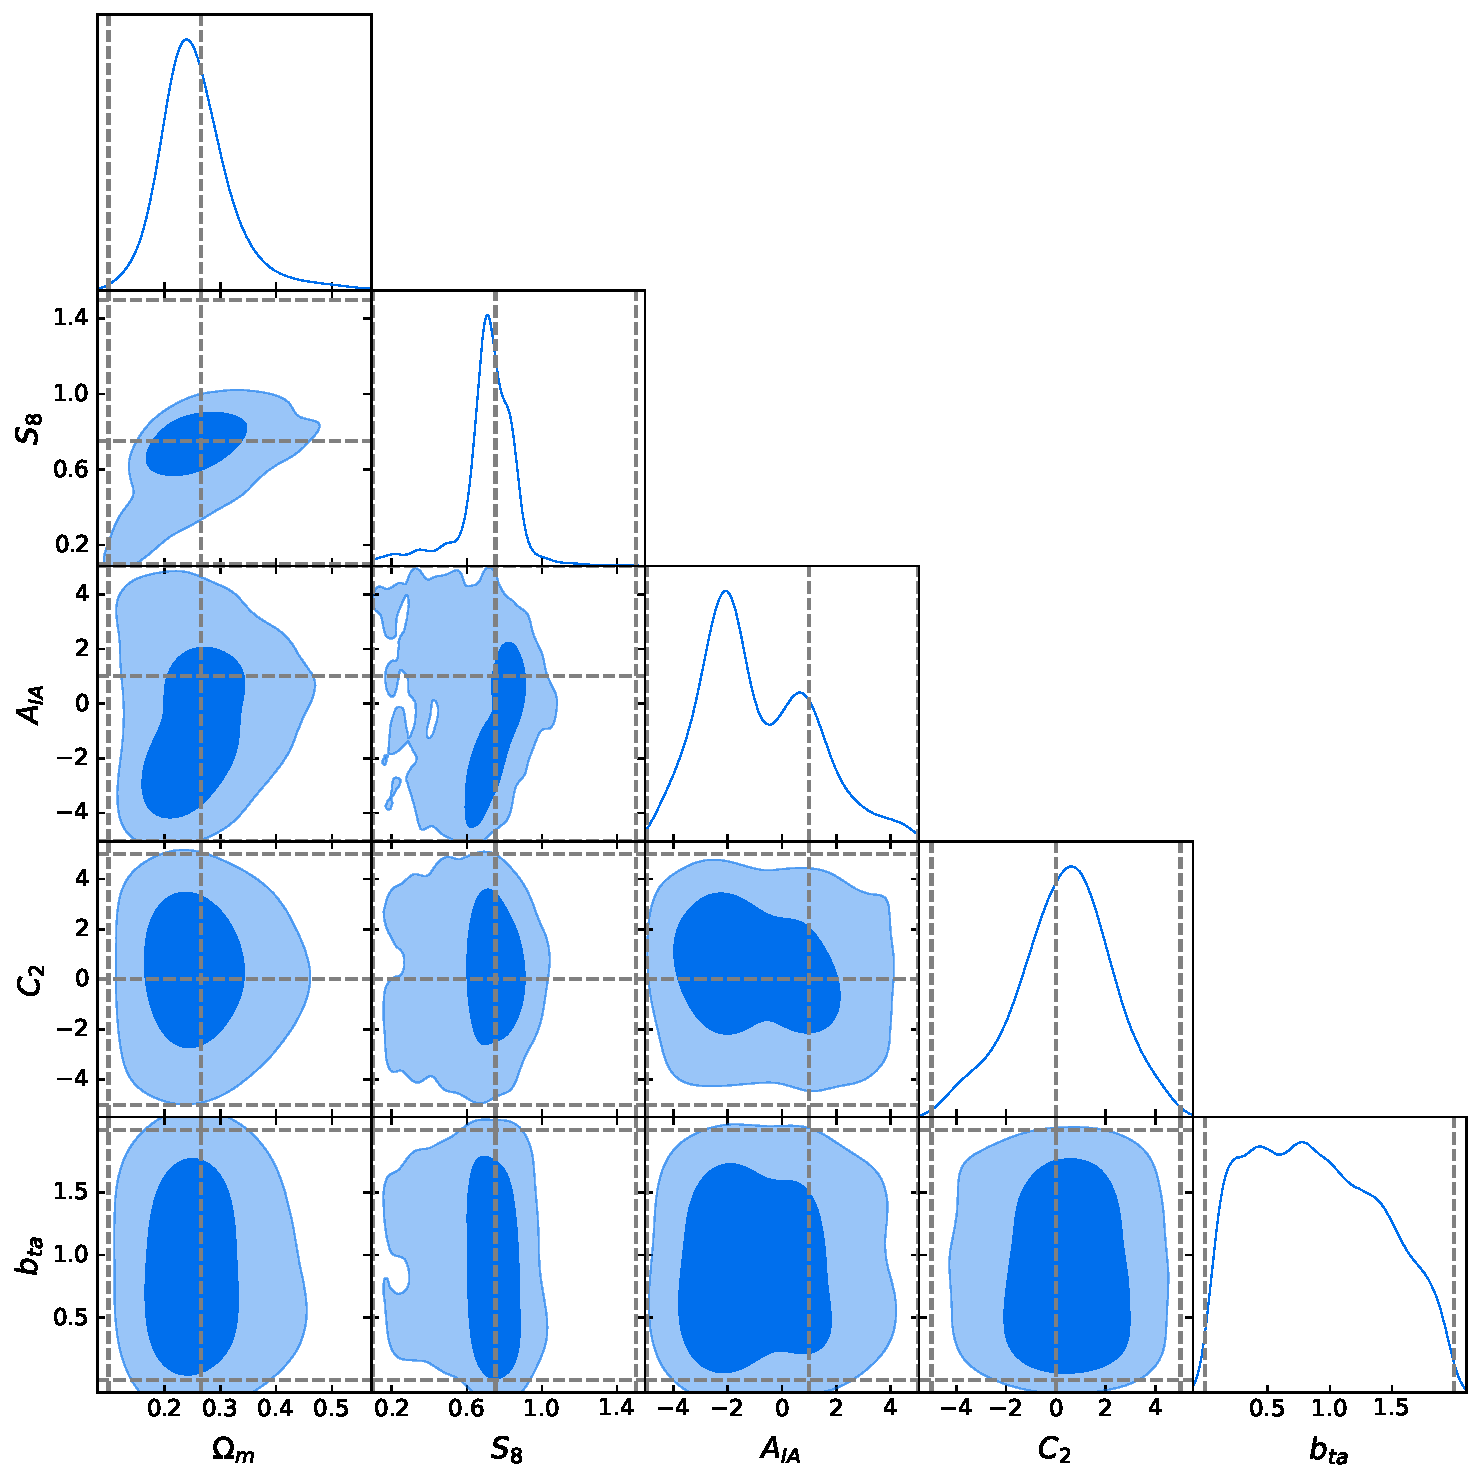
\includegraphics[width=\columnwidth]{graphs/triangle_nla_5D.pdf}
%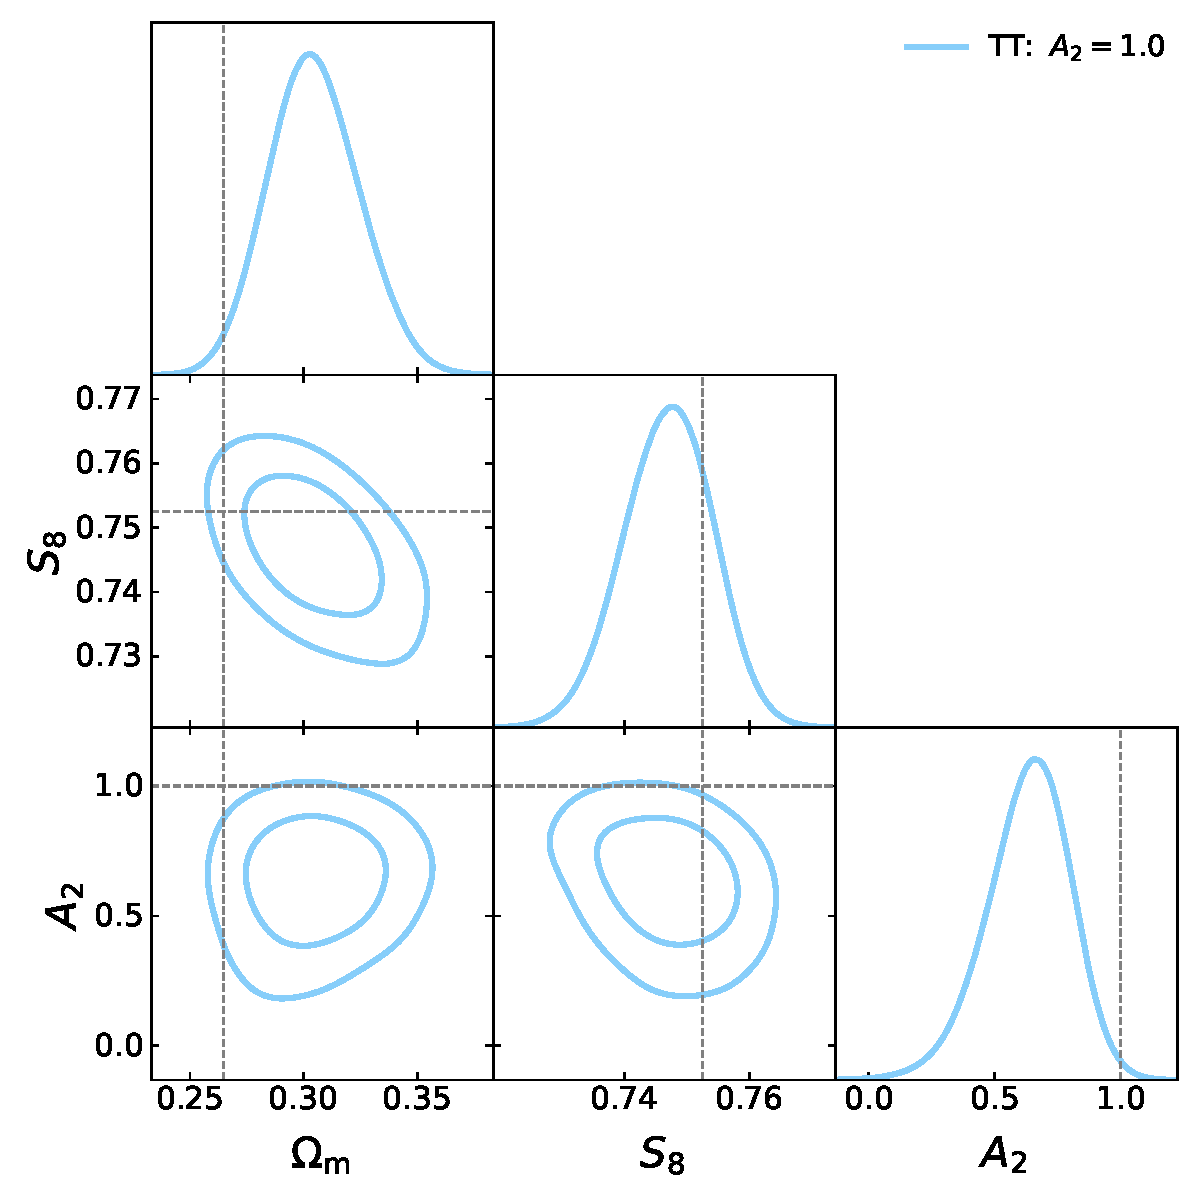
\includegraphics[width=\columnwidth]{graphs/TT_a2.pdf}
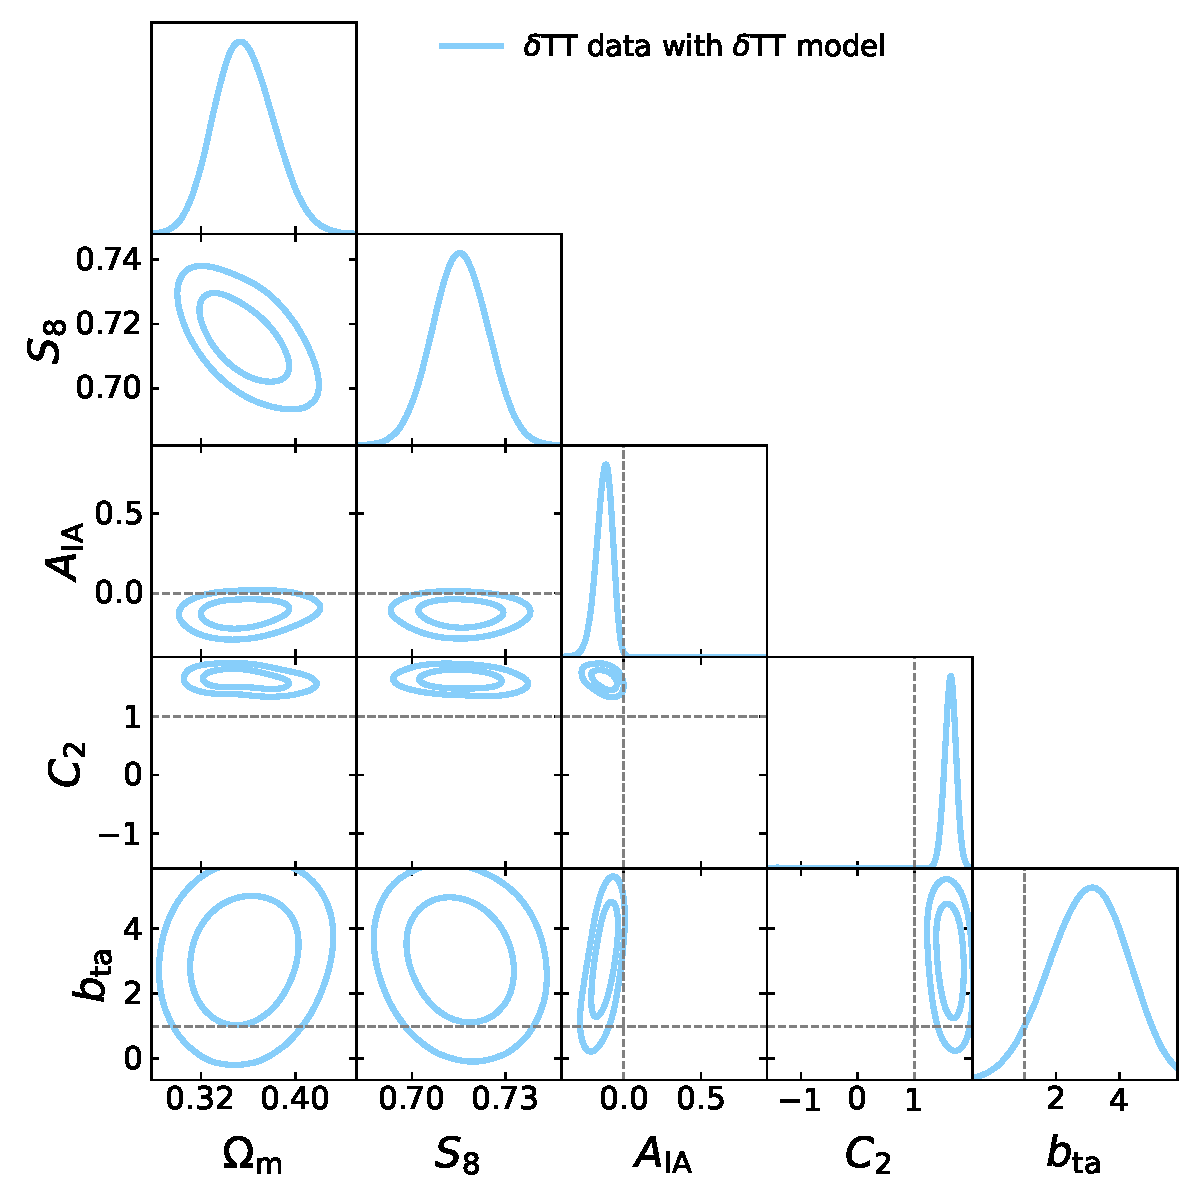
\includegraphics[width=\columnwidth]{graphs/deltaTT.pdf}
\caption{Cosmological inference from the $\delta$-TT-infused simulations, where either all three TATT parameters are varied.}
\label{fig:corner_deltatt}
\end{figure}
\begin{figure}
%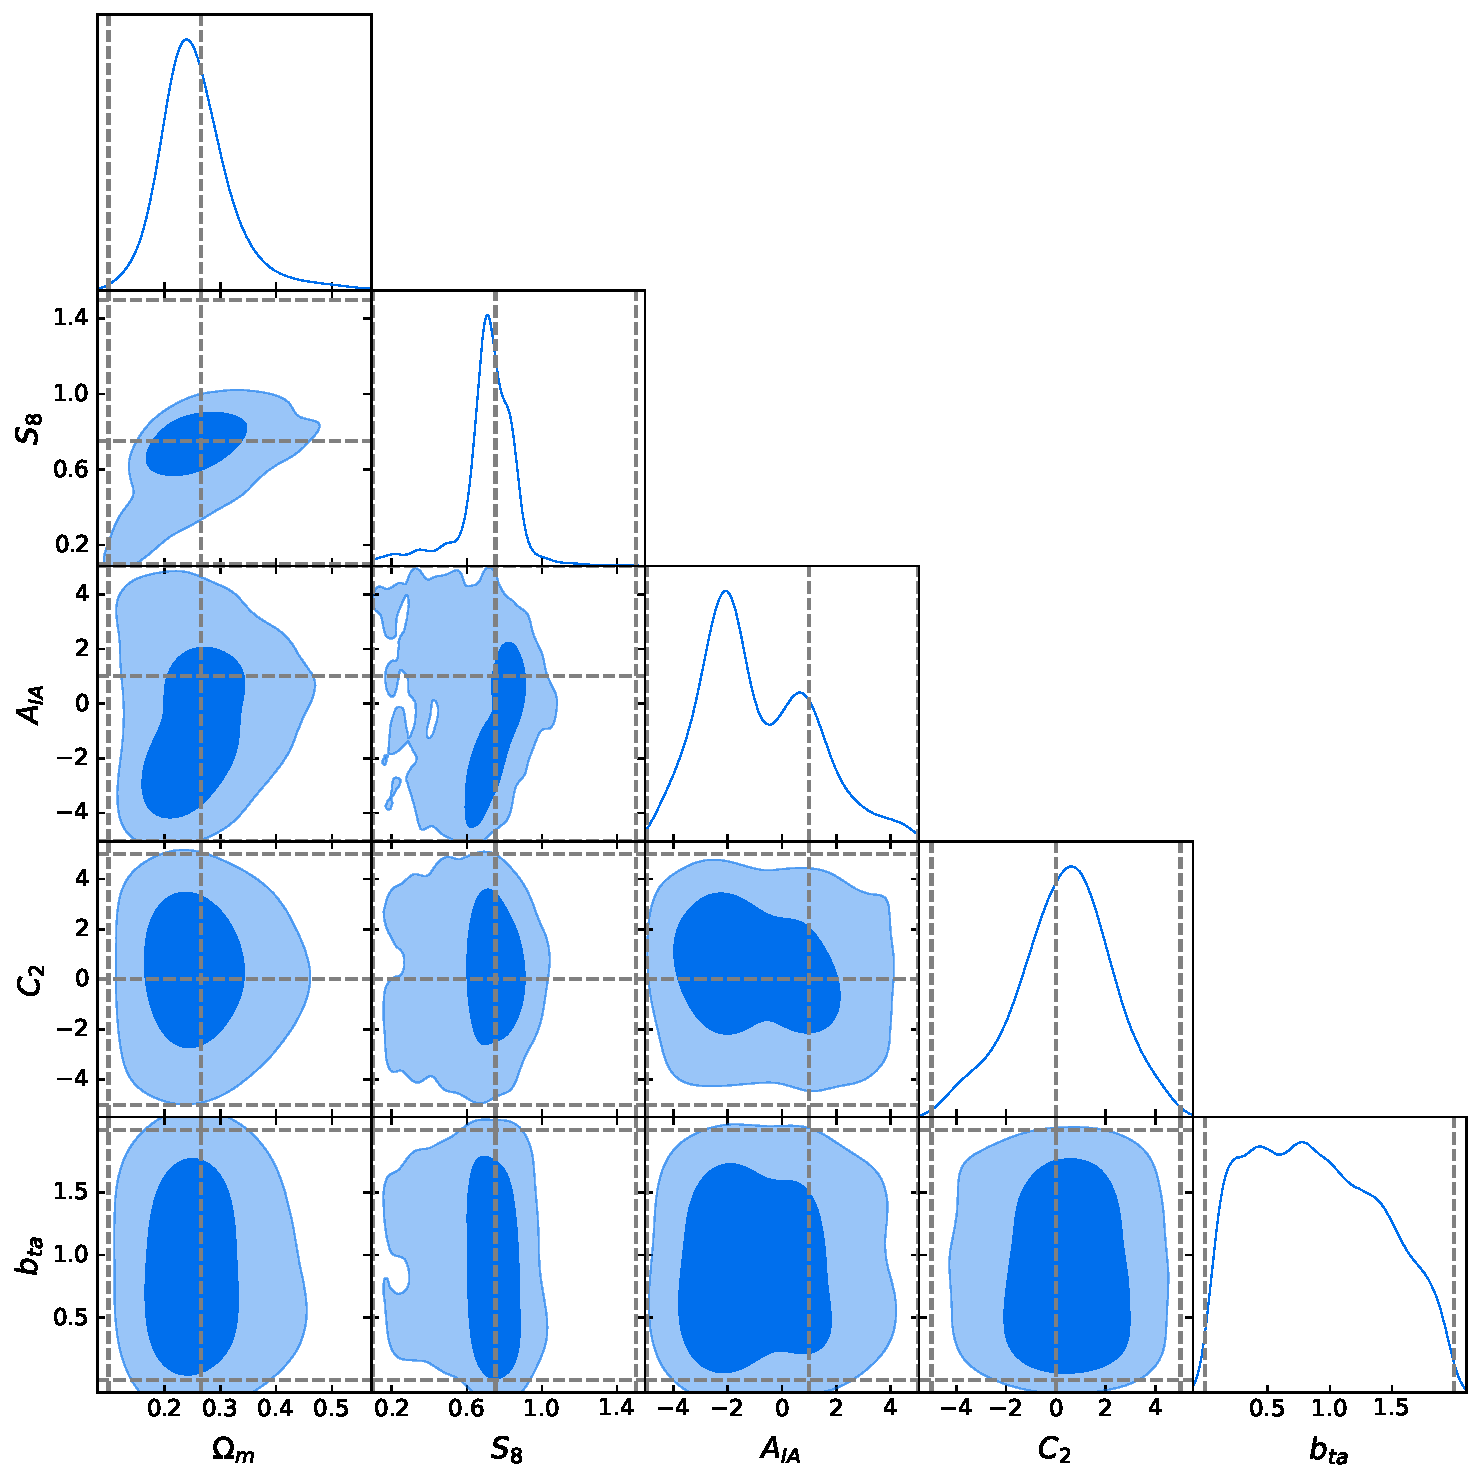
\includegraphics[width=\columnwidth]{graphs/triangle_nla_5D.pdf}
%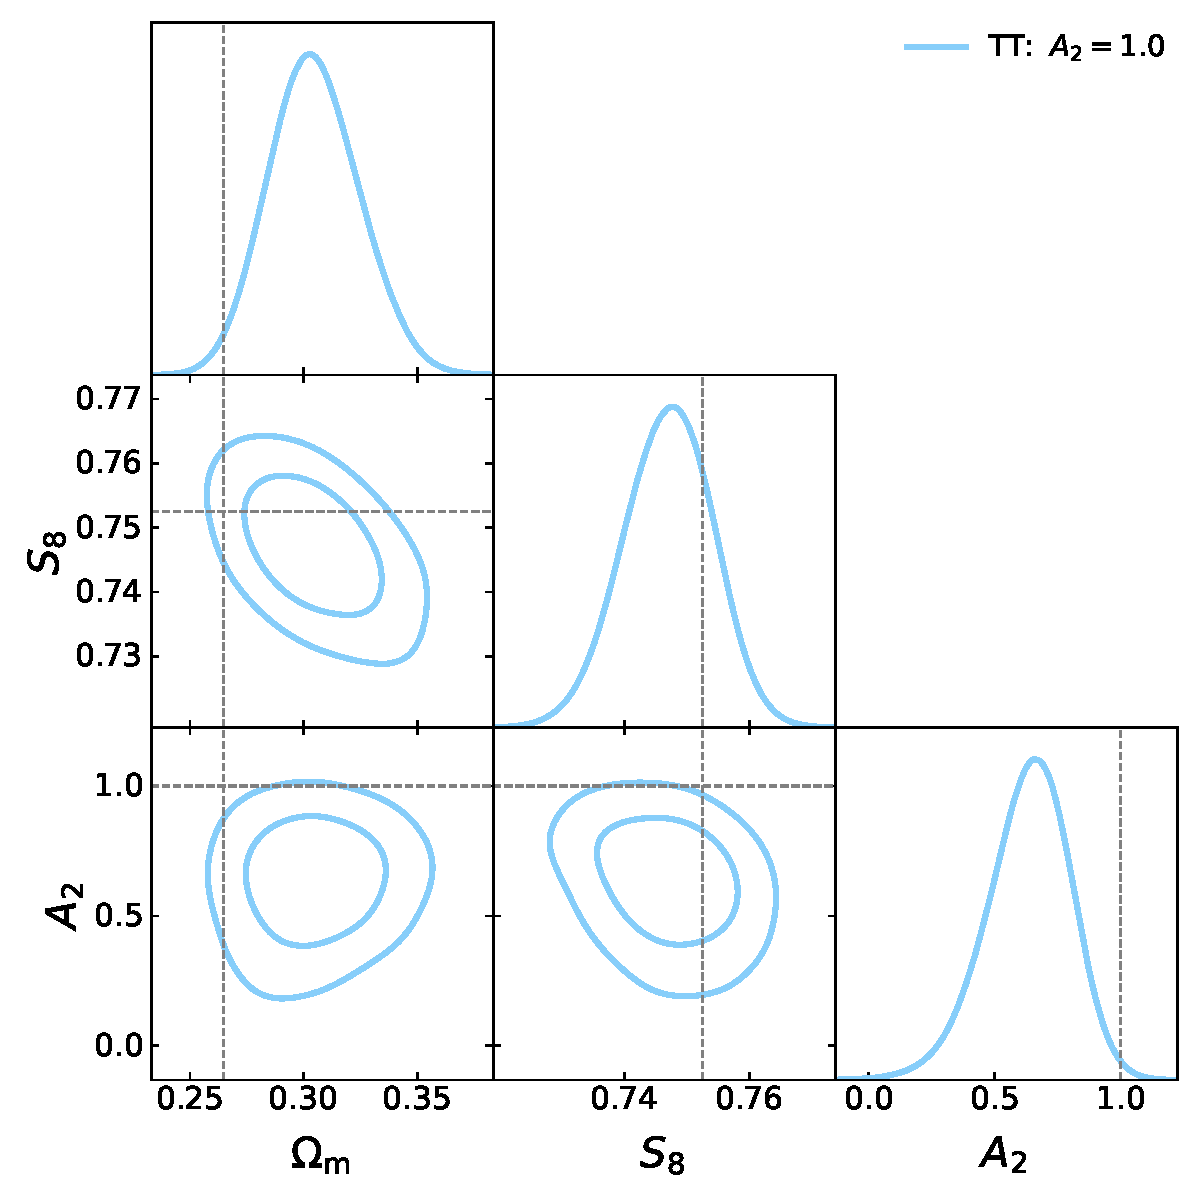
\includegraphics[width=\columnwidth]{graphs/TT_a2.pdf}
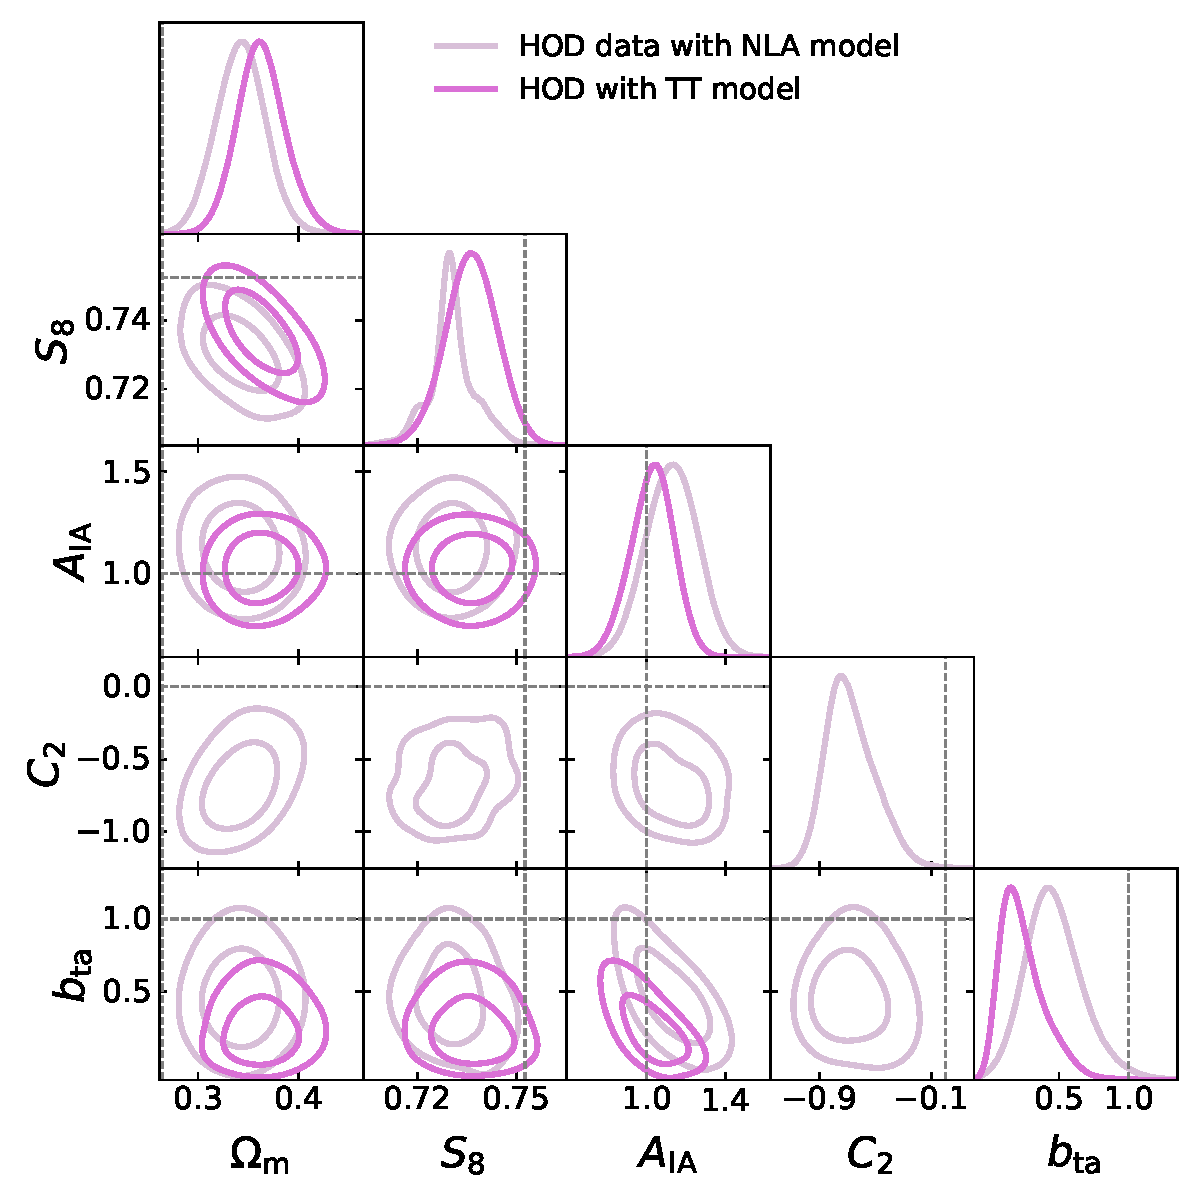
\includegraphics[width=\columnwidth]{graphs/HOD_NLA.pdf}
\caption{Cosmological inference from the HOD-NLA-infused simulations, where either all three TATT parameters are varied (light pink), or keeping $C_2=0$ fixed (dark pink) {\it (Niko, we need to confirm this, adjust the legend...)}.}
\label{fig:triangle_HOD_NLA_combo}
\end{figure}
 \begin{figure}
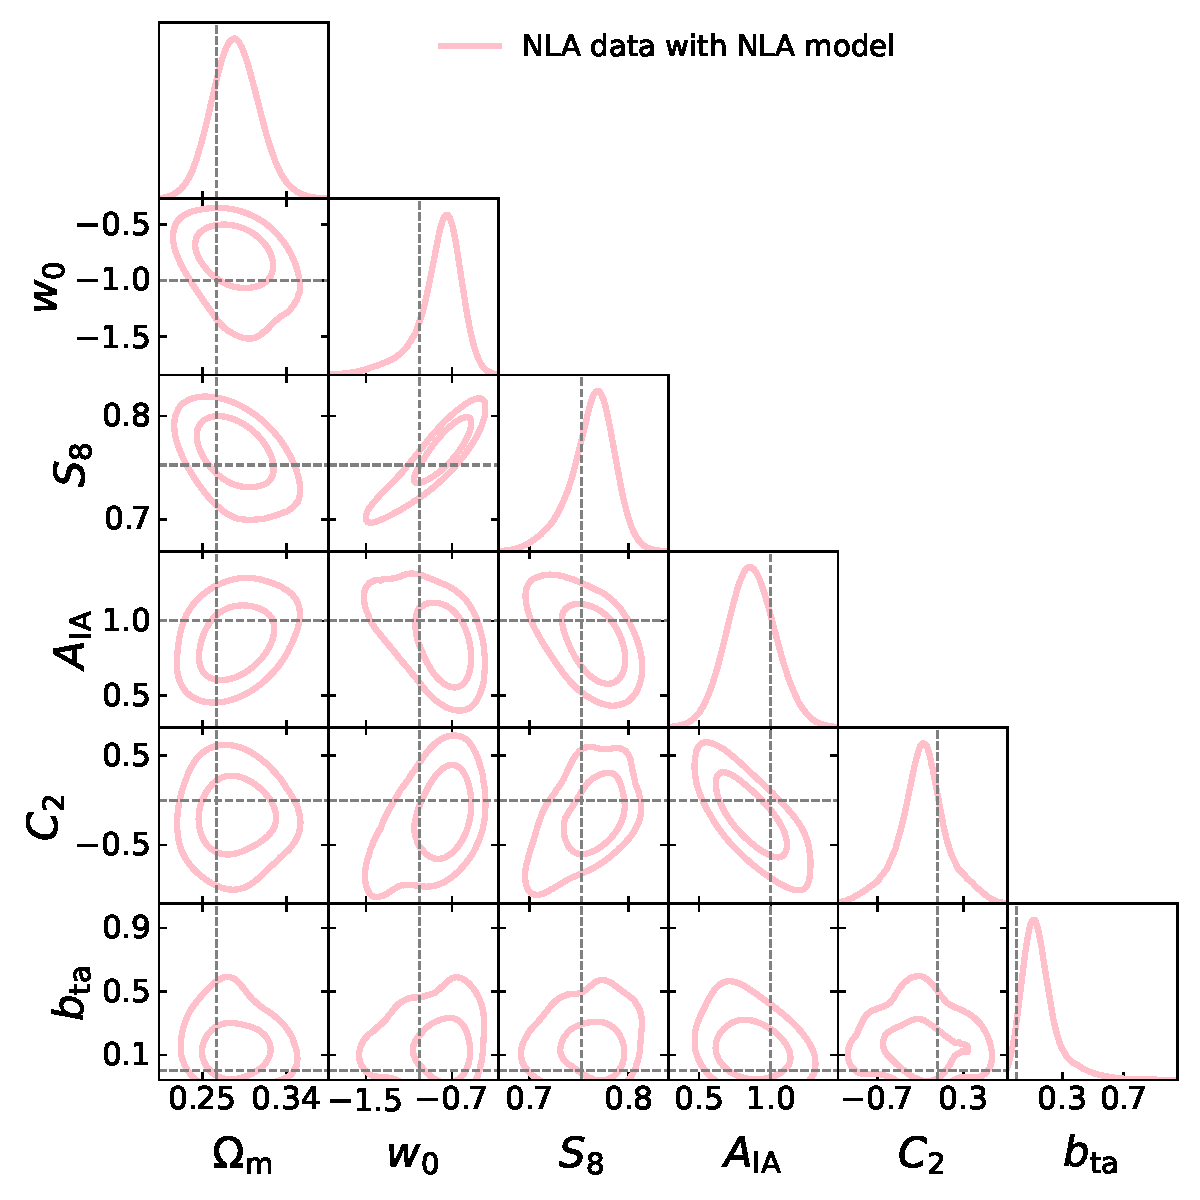
\includegraphics[width=\columnwidth]{graphs/NLA_w0.pdf}
\caption{Cosmological inference from the NLA-infused simulations, where all three TATT parameters are varied.}
\label{fig:corner_nla_w0}
\end{figure}

 
 The last section presented comparisons between measured and modelled signal, reaching generally an excellent agreement but highlighting some small differences. In order to quantify the importance of such differences in a cosmic shear analysis, our evaluation metric must be measurements of biases between the true and the inferred cosmological parameter. We achieve this by running nested likelihood sampling chains with {\sc multinest} \citep{Multinest}, which returns the posterior distributions $\mathcal{P}$ on the cosmological parameters $\boldsymbol \pi$ given a data vector $\boldsymbol  d$, a model vector $\boldsymbol m$, a covariance matrix C, and likelihood function $\mathcal L$ and a set of priors on the inferred parameters.  More precisely, we use a multivariate Gaussian likelihood, and ignore the standard cosmic shear systematic effects caused by photometric redshift errors, shape calibrations or baryon feedback \citep[see][for a recent example]{DESY3-KiDS1000}. We vary a subset of the vanilla $\Lambda$CDM cosmological parameters to establish the general accuracy; increasing the number of varied parameters can lead to a number of projection effects that complicate the interpretation. We therefore focus on varying the parameters best measured by lensing, namely $S_8$, $\Omega_{\rm m}$ and the IA parameters ($A_{\rm IA}, b_{\rm TA}, C_2$). We adopt wide flat priors for all of these, as detailed in Table \ref{table:priors}. 

With the precision of the Rubin data, small fluctuations in the data vectors can lead to significant shifts in the inferred cosmology, which is statistically  expected but makes the IA validation exercise more difficult to interpret. We therefore run our likelihood analyses on  the lowest three redshift bins, deliberately excluding the highest two as they contribute mostly to cosmological information, while we want here to learn more about the recovery of the IA sector. For the same reason we ignore shape noise here, which would only create additional scatter in the posteriors. We additionally exclude angular bins where the models probes highly non-linear scales, and select $\vartheta \in [2 ; 200]$ arcmin for $\xi_+$, and $\vartheta \in [20 ; 400]$ arcmin for $\xi_-$. These scales are highly affected by other systematic effects such as baryonic feedback \citep[see, e.g.][]{Semboloni11, HWVH15, 2020arXiv200715026H} and hence are often removed from the data vectors \citep[as in][]{DESY3_Amon}.


 The projected posteriors  are presented in Figs. \ref{fig:corner_nla_combo}-\ref{fig:corner_deltatt}, analysing simulated data from the six models introduced in Sec. \ref{sec:IA_th} model. In absence of IA contamination the inference from the simulated data is expected to yield posteriors on the cosmological parameters that are consistent with the input truth but not necessarily centred on it due to sample variance. We further dissect the analyses by varying either  one or  all three TATT parameters, highlighting some of the interesting degeneracies.   When analysing the NLA-infused data (Fig. \ref{fig:corner_nla_combo}), all cosmological and IA  parameters are accurately recovered, both for the NLA and TATT modelling. In the later case, the inferred values for $b_{\rm TA}$ and $C_2$ are consistent with zero, but we observe a strong degeneracy between  $A_{\rm IA}$ and  $C_2$ as also found in e.g. \citet[][\it  cite other papers?]{Paopiamsap2024}. 
The inferred  $\Omega_{\rm m}$ is slightly shifted to higher values, however this is not surprising given that cosmic shear alone is generally not able to constrain this parameter. $S_8$, however,  is well recovered, slightly on the high side. As expected, opening up the full TATT parameter space slightly degrades the constrains on cosmology, but no large shifts are observed. The $w$CDM chains also show an excellent convergence, as shown with the pink contours. {\it [update colour, merge figures 11 and 16]}.
 


 We next analyse the TT data with the TATT model in Fig. \ref{fig:triangle_tt_combo}, and  observe an accurate recovery of  $\Omega_{\rm m}$ and $S_8$, however the IA sector is strongly affected by the [$A_{\rm IA}; C_2$] degeneracy, which  pulls the posterior towards the NLA model, with values of $C_2$ consistent with 0 and preferring $A_{\rm IA}\sim 0.5$. When fixing $A_{\rm IA}$ and $b_{\rm TA}$ to the input truth however, the inferred $C_2$ just undershoots the input, pointing to residual differences between our implementation of the TT model and that calculated by TATT. Nevertheless, the fact that the cosmology is well recovered is promising, since ommiting completely the IA modelling would yield to catastrophic biases in $\Omega_{\rm m}$ and $S_8$. 


 As explained above, the extended NLA model infused in our simulations is not entirely well captured by the {\sc CosmoSIS} implementation, especially the $II$ term for the lowest redshift bins. This causes problems when inferring parameters with  {\sc CosmoSIS}, since the predictions attempt to compensate the difference in the IA model, leading to biases in the other parameters. Fig. \ref{fig:triangle_deltaNLA_combo} shows exactly this, failing to infer correctly most parameters. In this particular case,  $\Omega_{\rm m}$ and $S_8$ are only off by $2\sigma$, $A_{\rm IA}$ and $C_2$ are biased by 4-5$\sigma$, however $b_{\rm TA}$ is within 1$\sigma$. The $\delta$-TT model is even more affected by mis-modelling, with a 3$\sigma$ shift in both $\Omega_{\rm m}$ and $S_8$, as seen in Fig. \ref{fig:corner_deltatt}.
 
The infusion with the HOD-NLA model shows much larger deviations, largely driven by the sharp upward turn observed in auto-correlation at low redshifts, which also caused biases on the extended NLA. This causes biases of 2-3$\sigma$ in the cosmological parameters, notably lower $S_8$. In other works, if the  real world IA model was the extended-NLA or HOD-NLA and that we'd analyse it with the {\it cosmoSIS} implementation of  NLA or TATT, this would significantly contribute toward the existing $S_8$ tension \citep{S8tension}, in the same direction currently observed (i.e. late-time probes observe a lower $S_8$ value compared to CMB probes). We are careful here not to claim that this is the single cause of the current tension, but clear mis-model in the IA sector could contribute significantly. We do not include inference of the HOD-TT here since the level of mismatch is even worst.
  
 To summarise this section, aside from the NLA and TT, the infused IA models include terms that are different from the theory and hence lead to significant biases both in the cosmology and IA parameters.  
% We also show in Fig. \ref{fig:corner_nla_w0} the impact of promoting our $\Lambda$CDM inference to a $w$CDM inference, varying the dark energy  equation-of-state parameter $w$ in the range $[-2; -0.3]$. 
 These tests complete our validation of the IA-infusion pipeline, and we now look in the next section at the impact of IA on the weak lensing higher-order statistics mentioned in Sec. \ref{subsec:beyond-2pt}.
 
\section{Higher-order weak lensing statistics}
\label{sec:HOWLS}

... use the mocks from Table \ref{table:IAmodels} to compute derivatives. Show.
\section{Conclusions}
\label{sec:conclusion}
\section*{Acknowledgements}

JHD acknowledges support from an STFC Ernest Rutherford Fellowship (project reference ST/S004858/1). 
Ray-tracing computations were carried on the NERSC [acknowledgments] ... HACC [acknowledgements] ... {\it Outer Rim}[Acknowledgments]
\\

Some of the results in this paper have been derived using the {\sc healpy} and {\sc HEALPix} packages.
\\
\\
\\
{\footnotesize All authors contributed to the development and writing of this paper.
JHD led the analysis.... }
\section*{Data Availability}

 
%The SLICS numerical simulations can be found at http://slics.roe.ac.uk/, while the cosmo-SLICS can be made available upon request.
%The construction of our tomographic $n^i(z)$ can be reproduced in {\tt github...CCL\_SRD\_Niko}.
{[\it] Not sure what to make available here. Infusion code? Simulation products are DESC proprietary...}

%%%%% REFERENCES %%%%%

% The best way to enter references is to use BibTeX:
%\bibliographystyle{hapj}
\bibliographystyle{mnras}
\bibliography{references} 

%%%%% APPENDICES %%%%%

\appendix

\begin{figure*}
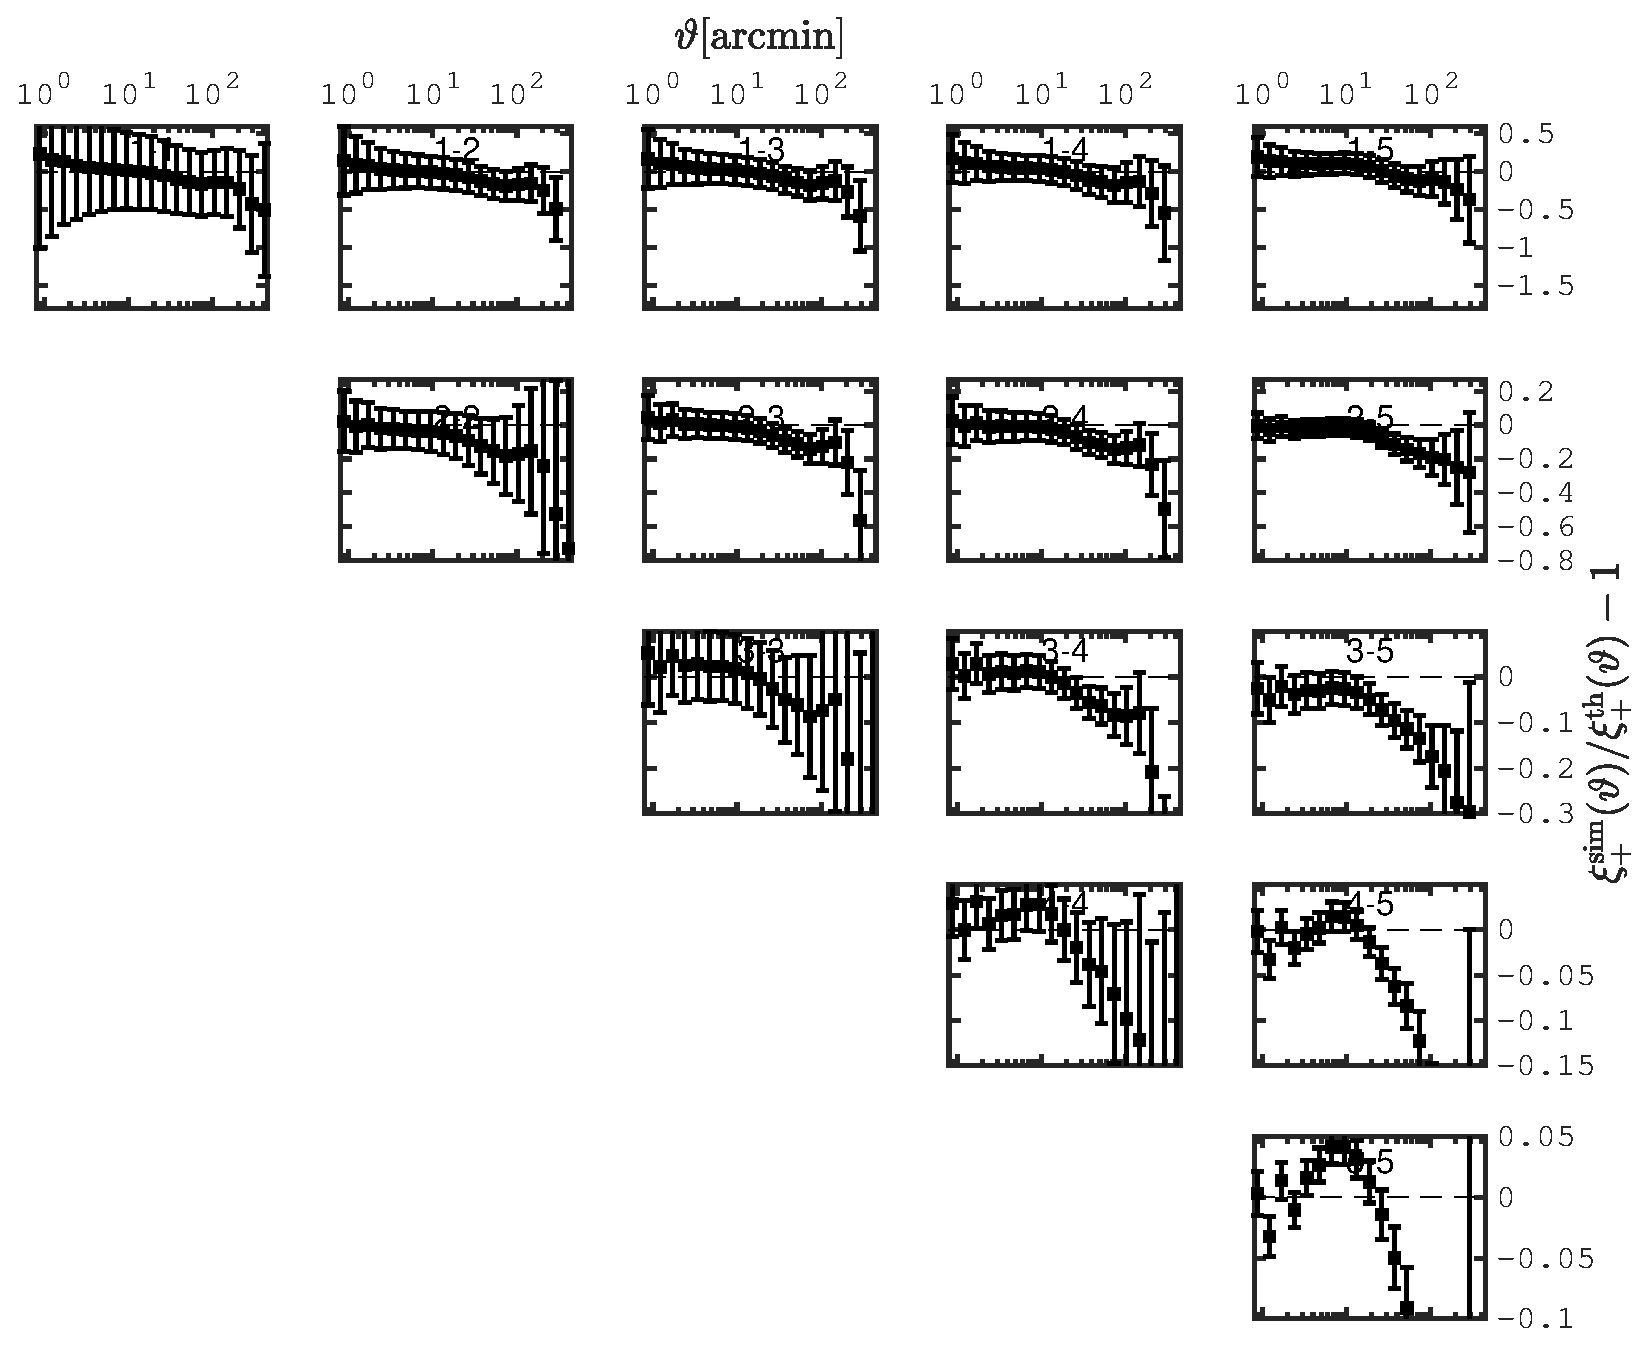
\includegraphics[width=\columnwidth]{graphs/xip_sims_vs_th.eps}
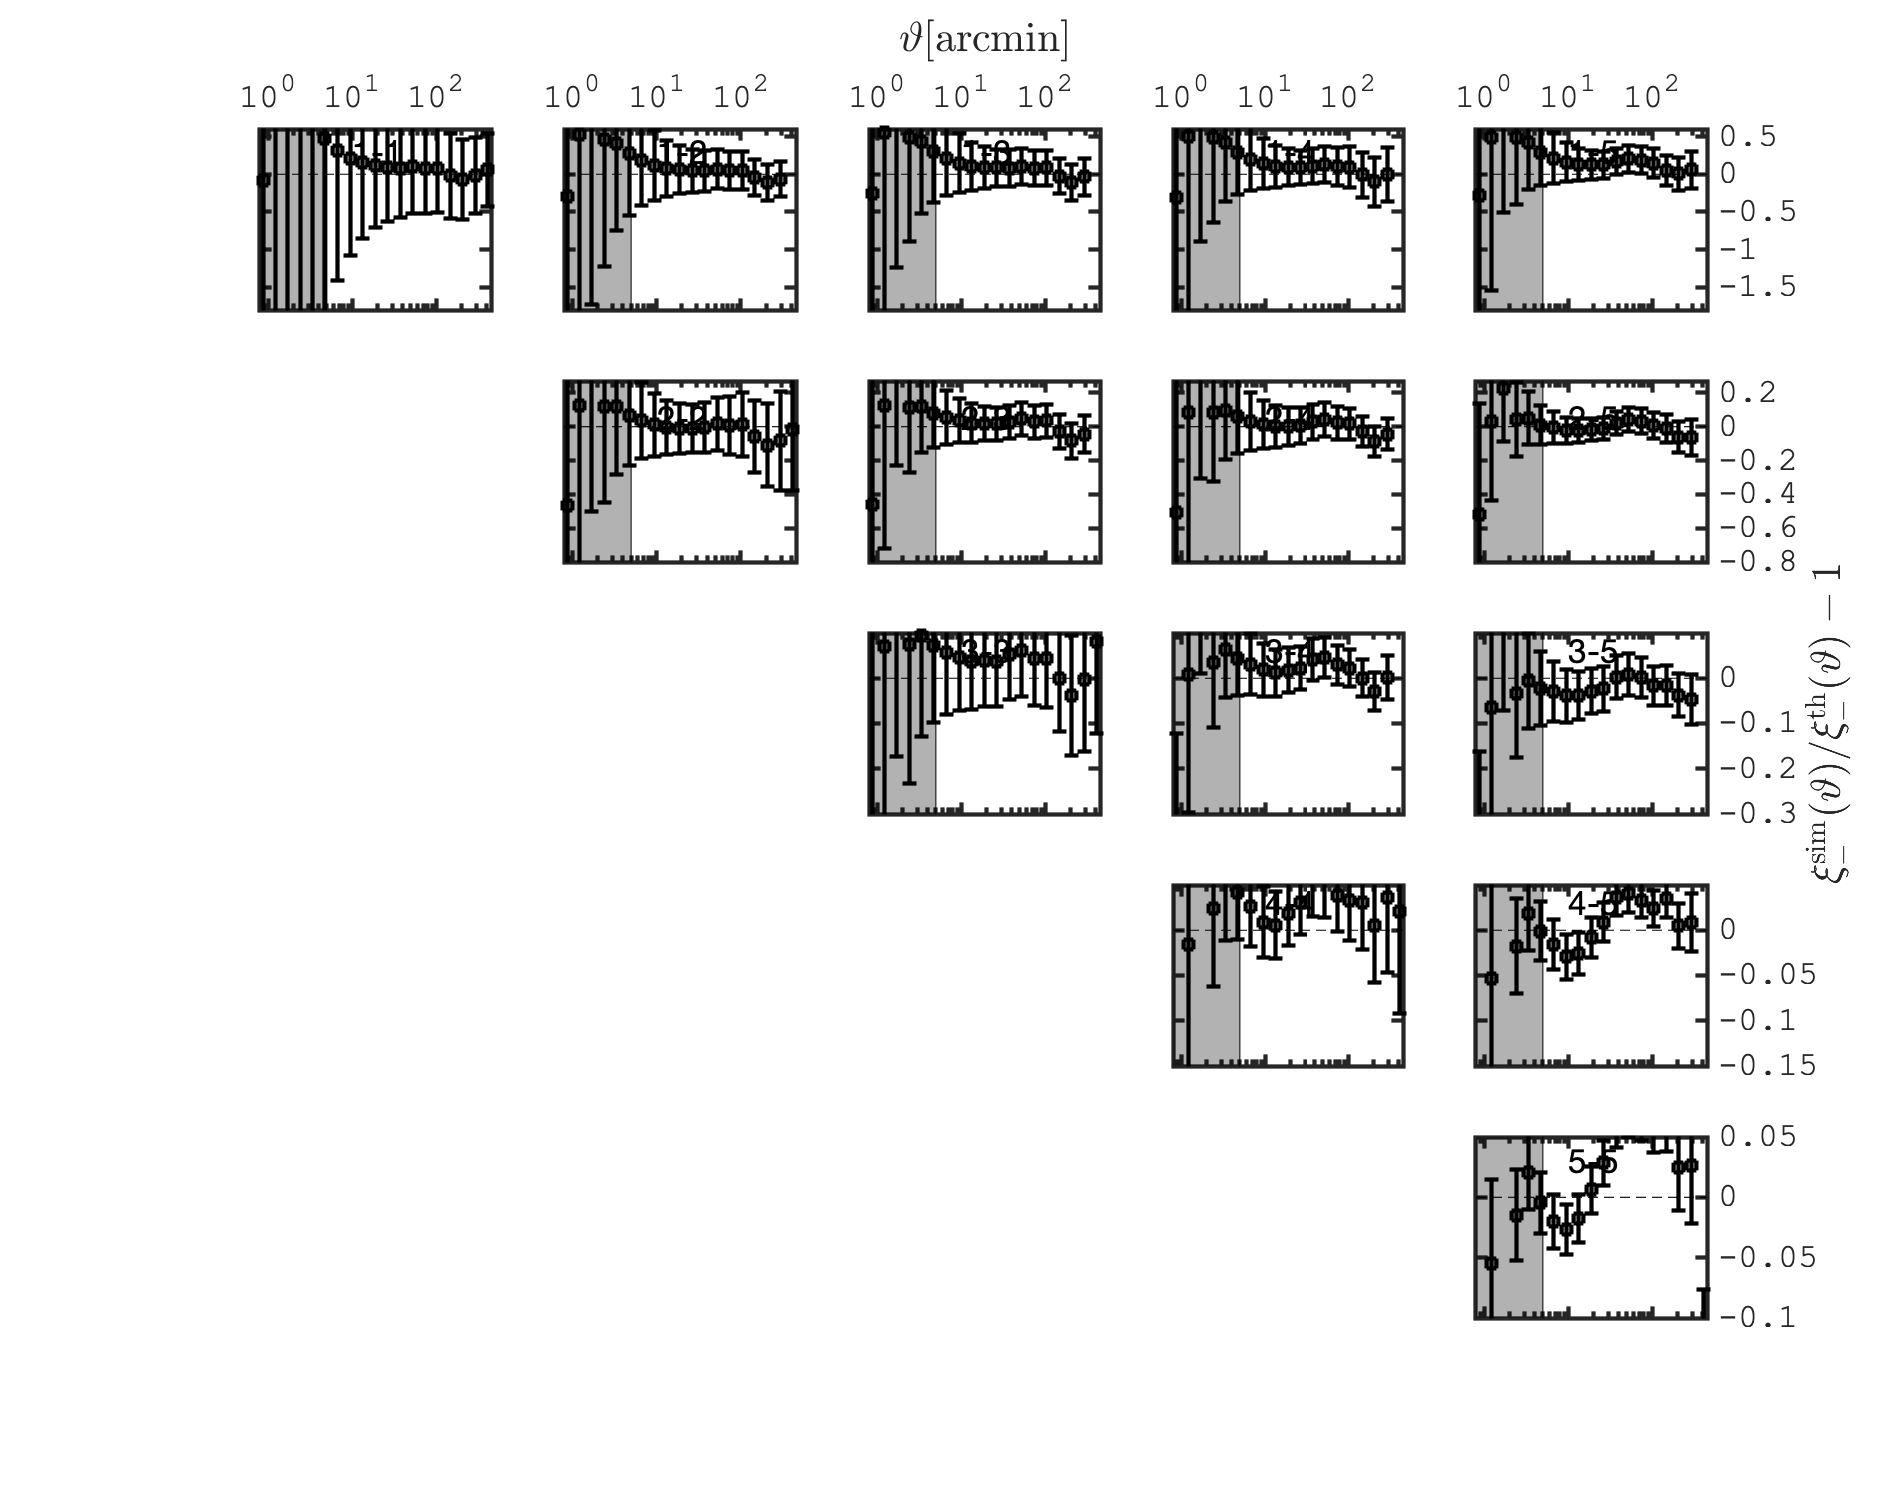
\includegraphics[width=\columnwidth]{graphs/xim_sims_vs_th.eps}
\caption{Fractional difference on $\xi_\pm$ between the measurements from SkySim5000 and the model predictions.  }
\label{fig:frac_err_sims_th}
\end{figure*}

\section{Projected Tidal Field}
\label{app:2d_TT}


\JHD{[To reword]} We derive in this Appendix...  
The prescription to assign an intrinsic alignment based on the projected tidal field, described in Eq. (\ref{eq:tidal_th}), involves the combinations $(s_{xx} - s_{yy})$ and $s_{xy}$, which therefore correspond to:
\begin{eqnarray}
 \widetilde{\epsilon}_1^{\rm IA} (\boldsymbol k_{\perp})  &\propto& \left(\frac{k_x^2 - k_y^2}{k^2} \right) \widetilde{\delta}_{\rm 2D}(\boldsymbol k_{\perp})\mathcal{G_{\rm 2D}}(\sigma_{\rm G})  \, ,\nonumber \\
 \widetilde{\epsilon}_2^{\rm IA} (\boldsymbol k_\perp)  &\propto& \left(\frac{k_x k_y}{k^2} \right) \widetilde {\delta}_{\rm 2D}(\boldsymbol k_\perp)\mathcal{G_{\rm 2D}}(\sigma_{\rm G}) 
 %\label{eq:sij}
\end{eqnarray}

Aside from the smoothing kernel, these are the same filters that are used for converting convergence maps to shear maps under the \citet[][KS hereafter]{KaiserSquires} inversion:
 \begin{eqnarray}
 \widetilde{\gamma_1} (\boldsymbol \ell)  = \left(\frac{k_x^2 - k_y^2}{k^2} \right) \widetilde {\kappa}(\boldsymbol \ell) \, , \hspace{1cm} \widetilde{\gamma_2} (\boldsymbol \ell)  = \left(\frac{k_x k_y}{k^2} \right) \widetilde {\kappa}(\boldsymbol \ell)
 %\label{eq:sij}
\end{eqnarray}
meaning that on can linearly combine the mass sheets with the correct coefficients and obtain intrinsic ellipticities from a normal KS inversion. 

Projecting out the $z$ components (e.i. $s_{0i}$=$s_{i0}$=0 for all $i$),  the tidal torque terms from Eq. (\ref{eq:tidal_th_TT}) can be expanded as:
 \begin{eqnarray}
\gamma^{\rm TT}_{ij}&=& C_2 \left[\sum_{k=x,y} s_{ik} s_{kj} -\frac{1}{3} \delta_{ij} s^2\right] \\
                                  &=&C_2 \left[ s_{ix}s_{xj}  + s_{iy}s_{yj}  -  \frac{1}{3} \delta_{ij} \left( s_{xx}^2 + s_{yy}^2 +2s_{xy}^2 \right)  \right] \, .
\end{eqnarray}
Specifically, this yields:
 \begin{eqnarray}
\gamma^{\rm TT}_{xx}&=& C_2 \left[\frac{2}{3}s_{xx}^2  -  \frac{1}{3}s_{yy}^2 + \frac{1}{3}s_{xy}^2 \right]\, ,  \nonumber \\
\gamma^{\rm TT}_{yy}&=& C_2 \left[-\frac{1}{3}s_{xx}^2  +  \frac{2}{3}s_{yy}^2 + \frac{1}{3}s_{xy}^2  \right]\, , \\
\gamma^{\rm TT}_{xy}&=& C_2 s_{xy}\left[s_{xx}+s_{yy}  \right]\, . \nonumber                                  
\end{eqnarray}
With the standard ellipticity definitions $\epsilon_1^{\rm TT}\equiv \gamma_{xx}^{\rm TT} - \gamma_{yy}^{\rm TT}$ and $\epsilon_2^{\rm TT}\equiv -2 \gamma_{xy}$, we obtain:
\begin{eqnarray}
\epsilon_1^{\rm TT} = C_2  \left[ s_{xx}^2 - s_{yy}^2\right] \, , \epsilon_2^{\rm TT} = -2 C_2 s_{xy}\left[s_{xx}+s_{yy}  \right]\, .
\end{eqnarray}
In the TATT model, the total intrinsic ellipticity component is therefore given by $\epsilon_{1/2}^{\rm IA} = \epsilon_{1/2}^{\rm TATT} = \epsilon_{1/2}^{\delta{\rm-NLA}} + \epsilon_{1/2}^{\rm TT}$.

% Don't change these lines
\bsp	% typesetting comment
\label{lastpage}
\end{document}

% End of mnras_template.tex